% Header
\renewcommand\evenpagerightmark{{\scshape\small Chapter 2}}
\renewcommand\oddpageleftmark{{\scshape\small Investigating the \si{TeV} scale}}

\renewcommand{\bibname}{References}

\hyphenation{}

\chapter[Investigating the \si{TeV} scale]%
{Investigating the \si{TeV} scale}
\label{chapt:2}

	Throughout history, physics experiment became more and more powerful in order to investigate finer details of nature to help understanding the building blocks of matter and the fundamental interactions that bind them in the microscopic world. Nowadays, the \acl{SM} of particle physics is the most accurate theory designed to explain the behaviour of particles and is able to make very precise predictions that are constantly verified. Nevertheless, some hints of new physics are visible as bricks are still missing to obtain a global description of the Universe.
	
	To highlight the limits of the SM and test the different alternative theories, evermore powerful machines are needed. It is in this context that the \acl{LHC} has been thought and built to accelerate and collide particles at energies exceeding anything that had been done before. Higher collision energies and high pile-up imply the use of enormous detectors to measure the properties of the interaction products. The \acl{CMS} is a multipurpose experiment that have been designed to study the proton-proton collisions of the LHC and give answers on various high-energy physics scenarios such as different \acf{SUSY} extensions to the \acl{SM} or Extra Dimensions models.
	
	This Chapter will be the occasion to go through the history of the \acl{SM} of Particle Physics to understand the research conducted today in \acf{HEP} facilities. From the discovery of the atom and of its inner structure to the development of the theories governing the fundamental interactions, all the elements leading to the construction SM will be discussed. Furthermore, highlights on the \acf{BSM} will be given to replace the document in the context of today's research.  Finally, a full description of the LHC and of the CMS detector will be provided.

\section{The \acl{SM} of Particle Physics}
\label{chapt2:sec:SM}

	In the early \St{21} century it is now widely accepted that matter is made of elementary blocks referred to as \textit{elementary particles}. The physics theory that classifies and describes the best the behaviour and interaction of such elementary particles is the so-called \acl{SM}. The SM formalizes three of the four fundamental interactions (electromagnetic, weak and strong interactions). Its development happened since the 1960s thanks to a strong collaboration between theoretical and experimental physicists.

	\subsection{A history of particle physics}
	\label{chapt2:ssec:history}
	
	The idea that nature is composed of elementary bricks, called \textit{atomism}, is not contemporary as it was already discussed by Indian or Greek philosophers during antiquity. In Greece, atomism has been rejected by \textit{Aristotelianism} as the existence of \textit{atoms} would imply the existence of a void that would violate the physical principles of Aristotle philosophy. Aristotelianism has been considered as a reference in the european area until the \Th{15} century. With the \textit{Rinascimento}, antic text and history started to be more deeply studied. The re-discovery of Platon's philosophy allowed opening the door to alternative theories and give a new approach to natural sciences where experimentation would become central. A new era of knowledge was starting. By the beginning of the \Th{17} century, atomism was re-discovered by philosophers. The very first attempt at estimating the number of \textit{particles} in a volume was provided by Magnenus in 1646 by calculating that the number of \textit{particles} in a stick of incense~\cite{MAGNEGNUS1646}. He found a value of the order of $10^{18}$ simply by considering the time necessary to smell it everywhere in a large church after the stick was lit on. It is now known that this number only falls short only by 1 order of magnitude.

	\begin{figure}[H]
		\centering
		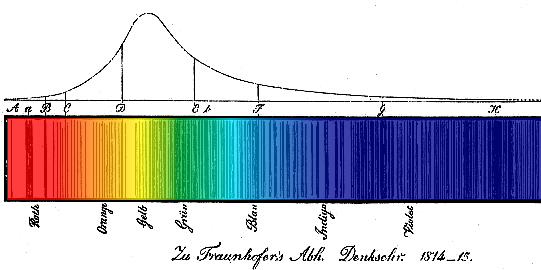
\includegraphics[width=0.7\linewidth]{fig/chapt2/Fraunhofer.jpg}
		\caption{\label{fig:spectral-lines} Solar spectrum with spectral lines as it visually appeared to Fraunhofer.}
	\end{figure}
	
	An alternative philosophy to atomism popularized by Descartes was \textit{corpuscularianism}. Built on ever divisible corpuscles, contrary to atoms, its principles were mainly used by alchemists like Newton who would later develop a corpuscular theory of light. Boyle combined together ideas of both atomism or corpuscularianism leading to mechanical philosophy. The \Th{18} century has seen the development of engineering providing philosophical thought experiments with repeatable demonstration and a new point of view to explain the composition of matter. Lavoisier greatly contributed to chemistry and atomism by publishing in 1789 a list of 33 chemical elements corresponding to what are now called \textit{atoms}~\cite{LAVOISIER1789}. In the early \Th{19} century Dalton summarized the knowledge on composition of matter~\cite{DALTON1808}. In his atomic model, the atoms are ball-like constituents of the chemical elements. All atoms of a given element are identical, in size, mass, and other properties while the atoms of different elements differ. He also considered that atoms cannot be divided into smaller particles, created nor destroyed and that they combine into chemical compounds. The essence of chemical reaction was then the combination, separation or rearrangement of atoms. Soon after, Fraunhofer invented the spectrometer and discovered the spectral lines in the sunlight spectrum, as showed in Figure~\ref{fig:spectral-lines}~\cite{FRAUNHOFER1814}. These were later linked to the absorption by chemical elements present in the solar atmosphere by Kirchhoff and Bunsen. The rise of atomic physics, chemistry and mathematical formalism unraveled the different atomic elements and ultimately, the \Th{20} century saw the very first sub-atomic particles.
	
	\subsubsection*{Discovery of the inner structure of the atom}
	\label{chapt2:sssec:atomstructure}

	\begin{figure}[H]
		\centering
		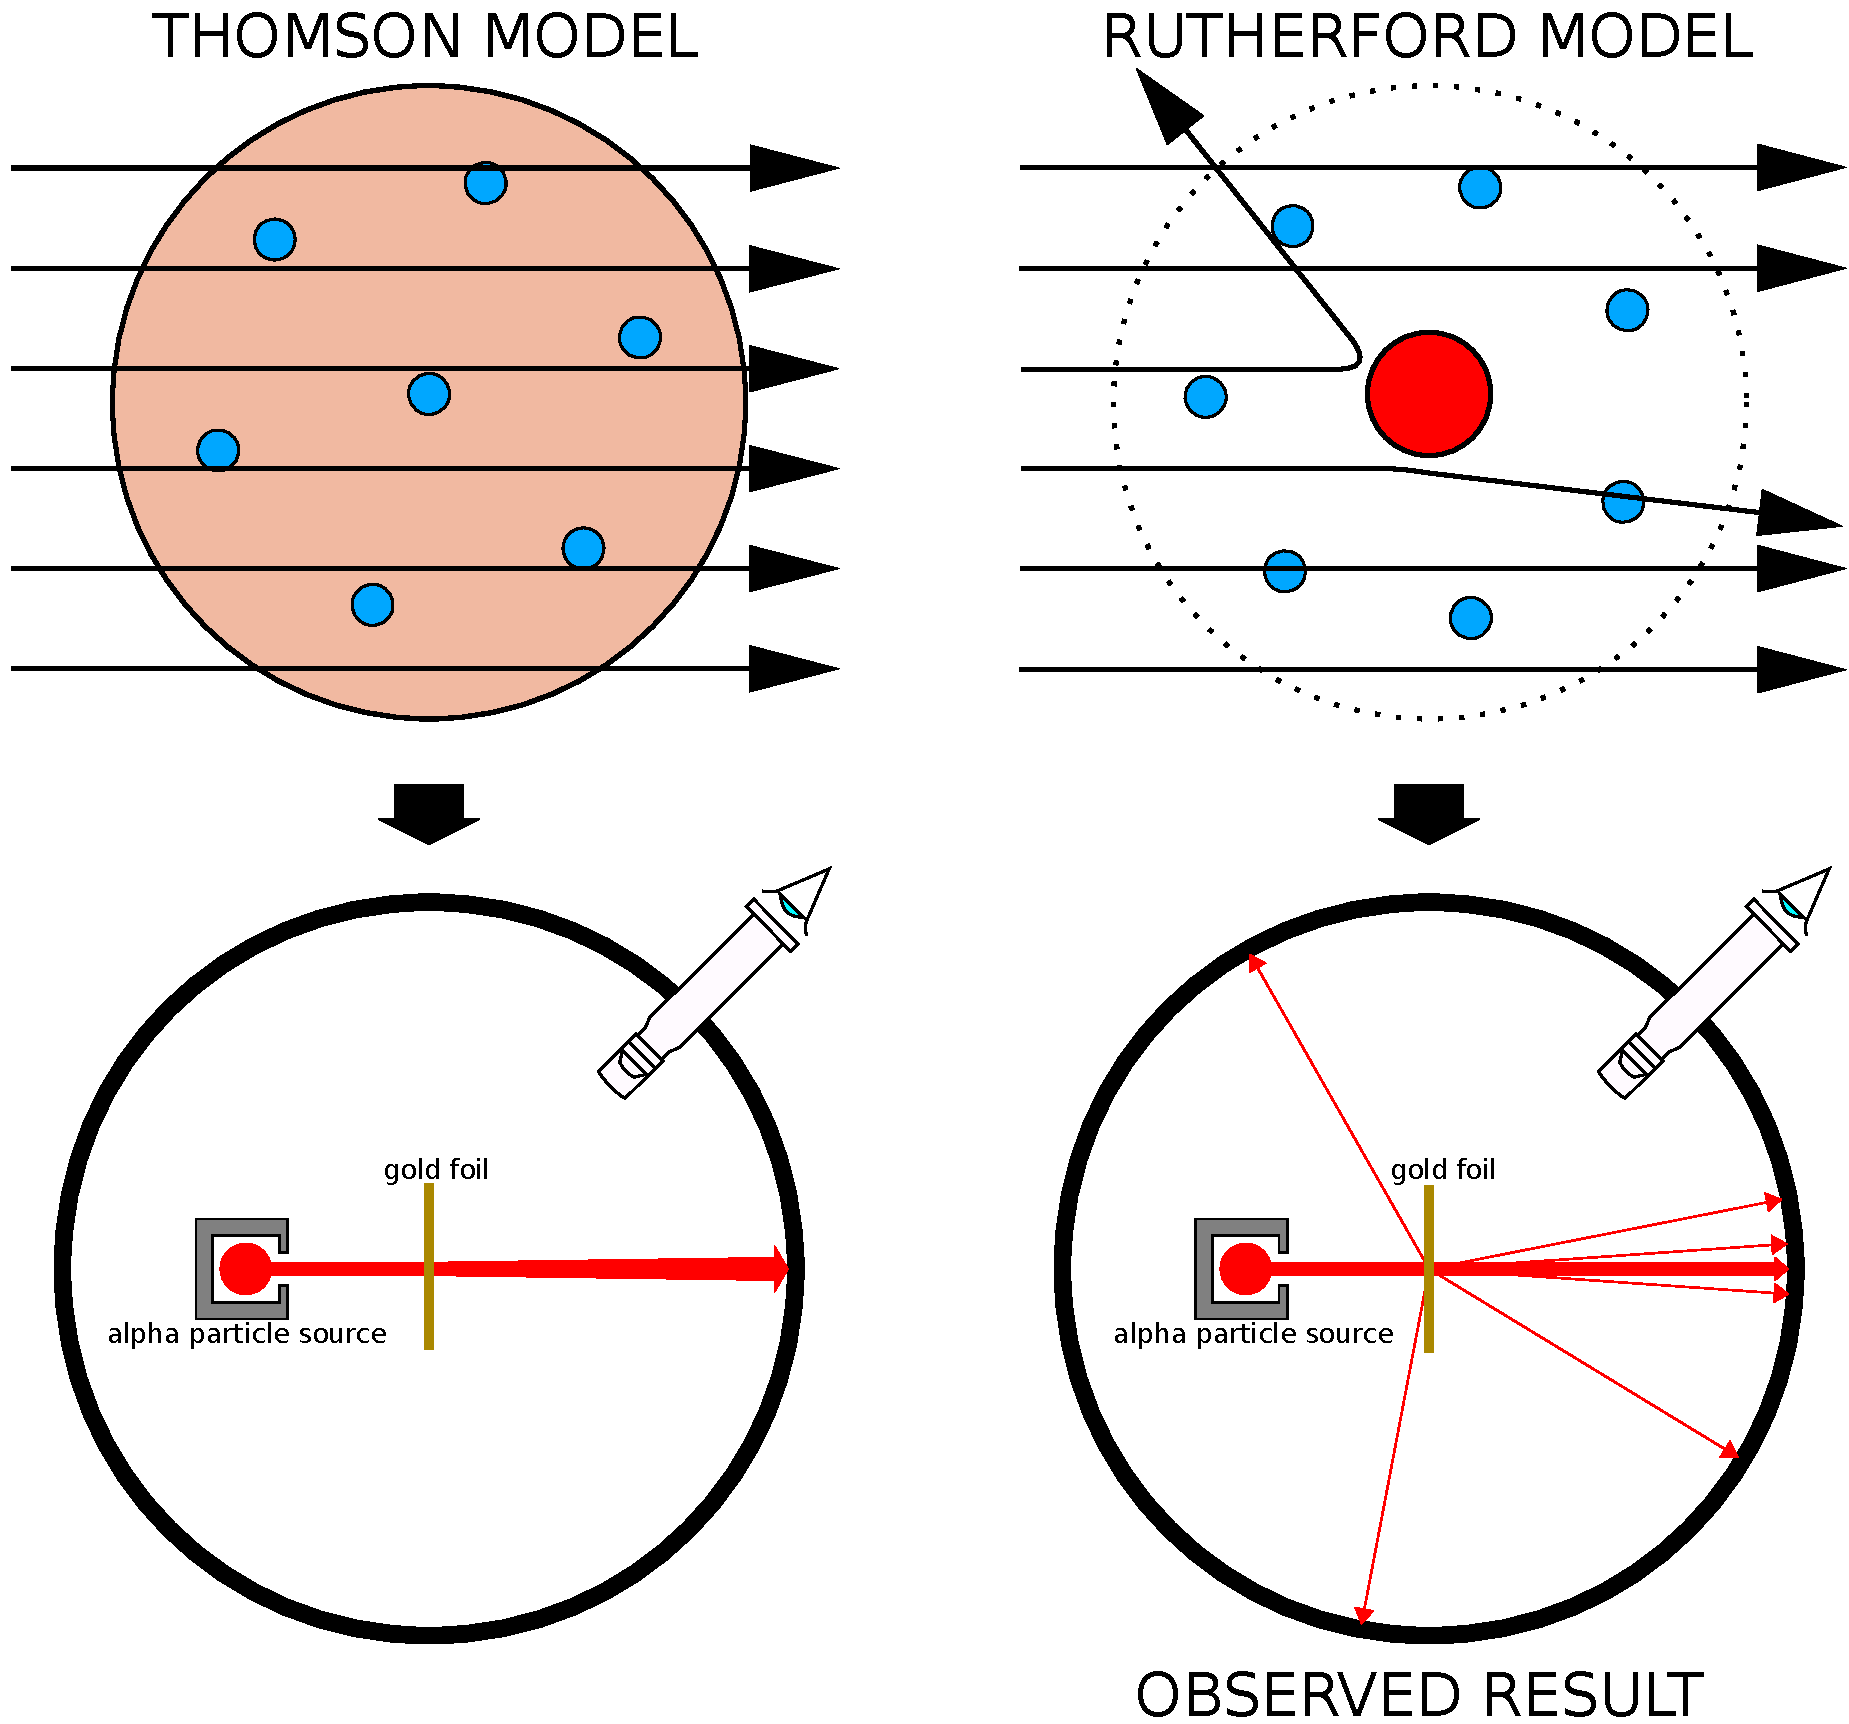
\includegraphics[width=\plotwidth]{fig/chapt2/Thomson_Rutherford_atoms.pdf}
		\caption{\label{fig:Atom_models} Through the gold foil experiment, Rutherford could show that most of the mass of atoms was contained in a positively charged nucleus and could then propose a more accurate atomic model than that of Thomson.}
	\end{figure}
	
	The negatively charged \textit{electron} was the first to be discovered in 1897 by Thomson after three decades of research on cathode rays~\cite{THOMSON1897}. He proved that the electrification observed in an electroscope, as reported by Perrin~\cite{PERRIN1895}, was due to the rays themselves. Hence, they had to be composed of electrically charged particles. In 1900, Becquerel showed the \textit{beta rays} emitted by radium had the same charge over mass ratio as was measured by Thomson for cathode rays, pointing to electrons as a constituent of atoms~\cite{BECQUEREL1900}. This discovery leads to Thomson's plum pudding atomic model in which electrons are embed into a uniform positively charged atom~\cite{THOMSON1904}. In 1907, Rutherford and Royds showed that \textit{alpha} particles were helium ions~\cite{RUTHERFORD1908}. Indeed, once captured in a tube and subjected to an electric spark causing an electron avalanche, they could combine with two electrons to form a $^4$He.
	
	This discovery was directly followed by the constraint of the atom structure in between 1908 and 1913 through the Geiger–Marsden gold foil experiments in which the deflection angle of alpha particles fired at a very thin gold foil was measured~\cite{GEIGER1908,GEIGER1909,GEIGER1910,GEIGER1913}. It highlighted that atoms were mainly empty with nearly all their mass contained into a tiny positively charged \textit{nucleus}. With these two observations, Rutherford could formulate the Rutherford planetary model of the atom in 1911~\cite{RUTHERFORD1911}, shown together with the Thomson plum pudding model in Figure~\ref{fig:Atom_models}. The link between atomic number and number of positive and negative charges contained into the atoms would fast be understood. Hence, the different kinds of element transmutations appeared to be purely nuclear processes making clear that the electromagnetic nature of chemical transformations could not possibly change nuclei. A new branch in physics appeared to exclusively study nuclei: \textit{nuclear physics}. By studying alpha emission and the product of their interaction with nitrogen gas, Rutherford reported in 1919 the very first nuclear reaction~\cite{RUTHERFORD1919}. It leads to the discovery that the hydrogen nucleus was composed of a single positively charged particle that was later baptised \textit{proton}~\cite{MASSON1921}. This idea came from 1815 Prout's hypothesis proposing that all atoms are composed of \textit{"protyles"} (i.e. hydrogen atoms)~\cite{PROUT1815,PROUT1816}. By using scintillation detectors, Rutherford could highlight typical hydrogen nuclei signature and understand that the impact of alpha particles with nitrogen would knock out a hydrogen nucleus and produce an oxygen 17, as showed in Formula~\ref{eq:nuclear} and would then postulate that protons are building bricks of all elements.
	
	\begin{equation}
		\label{eq:nuclear}
		^{14}N + \alpha \rightarrow ^{17}O + p
	\end{equation}
	
	With this assumption and the discovery of \textit{isotopes} together with Aston, elements with identical atomic number but different masses, Rutherford proposed that all elements' nuclei but hydrogen are composed of both charged particles, protons, and of chargeless particles, which he called \textit{neutrons}~\cite{RUTHERFORD1920,MASSON1921}. These neutral particles helped maintaining nuclei as one, as charged protons were likely to electrostatically repulse each other. He then introduced the idea of a new force, a \textit{nuclear} force. The first idea concerning neutrons was a bond state of protons and electrons as it was known that the beta decay, emitting electrons, was taking place in the nucleus. However, it was then shown that electrons being confined into the nucleus would hardly be possible due to Heisenberg's uncertainty principle. Finally, in 1932, following the discovery of a new neutral radiation, Chadwick could discover the neutron as an uncharged particle with a mass similar to that of the proton which would solve the nucleus puzzle~\cite{BOTHE1930,BOTHE1932,CURIE1932,CHADWICK1932,CHADWICK1933}.
	
	\subsubsection*{Development of the \acl{QED}}
	\label{chapt2:sssec:QED}
	
	Historically, the development of the quantum theory revolved around the question of emission and absorption of discrete amount of energy through light. Einstein used the initial intuition of Planck about the black-body radiation to develop in 1905 a model to explain the photoelectric effect in which light was described by discrete \textit{quanta} now called \textit{photons}~\cite{PLANK1900,EINSTEIN1905PHOTO}. For this model, Einstein introduced the concept of wave-particle duality as classical theory was not able to describe the phenomenon. With the new understanding of atoms and of their structure, classical theories also proved unable to explain atoms' stability. Indeed, using classical mechanics, electrons orbiting around a nucleus should radiate an energy proportional to their angular momentum and hence, loose energy through time and the spectrum of energy emission should then be continuous. However, it was known since the \Th{19} century and the discovery of spectral lines that the emission spectrum of material was discrete~\cite{FRAUNHOFER1814}.
	
\begingroup\setlength{\intextsep}{0pt}\setlength{\columnsep}{15pt}
	
	\begin{wrapfigure}{r}{0.45\linewidth}
		\begin{minipage}{\linewidth}
			\centering\captionsetup[subfigure]{justification=centering}
			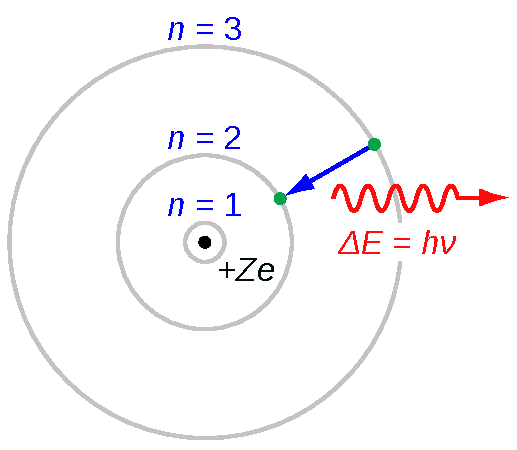
\includegraphics[width=.65\linewidth]{fig/chapt2/Bohr_atom_model.pdf}
			\subcaption{\label{fig:quantum-numbers:A}}
			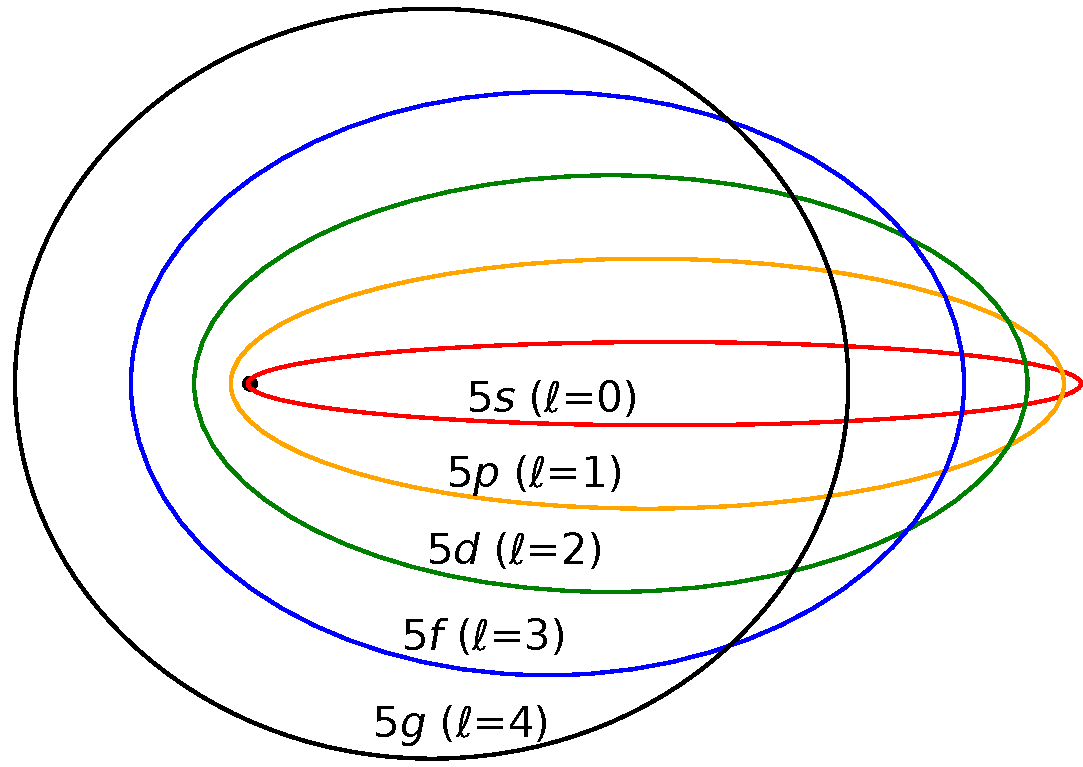
\includegraphics[width=.85\linewidth]{fig/chapt2/Sommerfeld_ellipses.pdf}
			\subcaption{\label{fig:quantum-numbers:B}}
			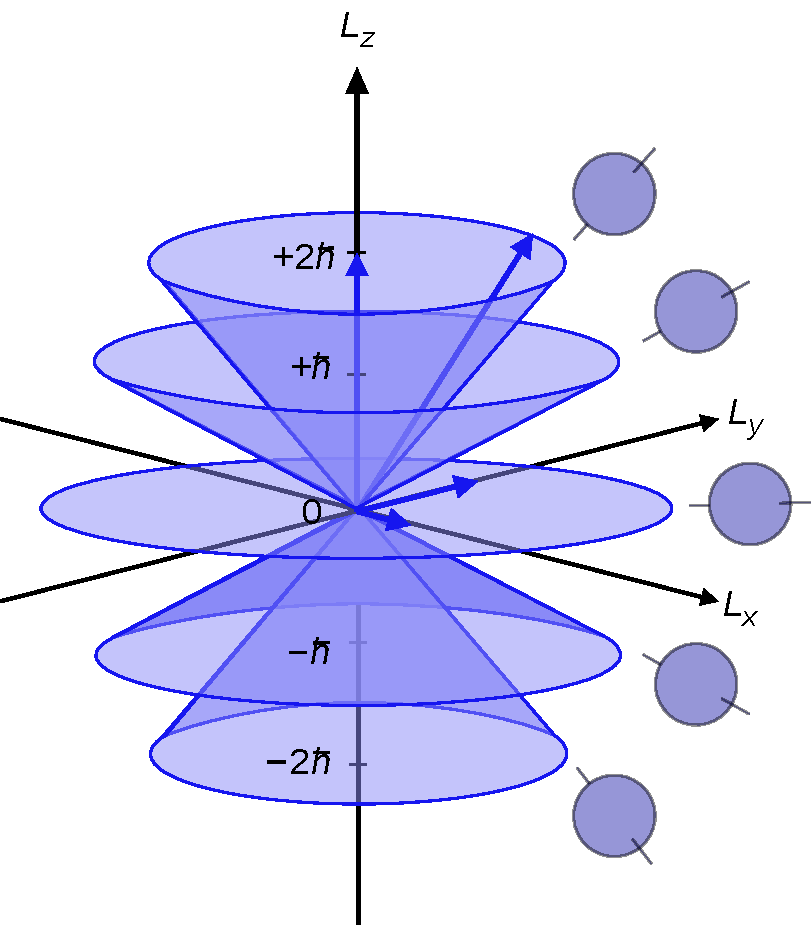
\includegraphics[width=.8\linewidth]{fig/chapt2/Vector_model_of_orbital_angular_momentum.pdf}
			\subcaption{\label{fig:quantum-numbers:C}}
		\end{minipage}
		\caption{\label{fig:quantum-numbers} Figure~\ref{fig:quantum-numbers:A}: The orbits in which the electron may travel according to the Borh model of the hydrogen atom. An electron jumps between orbits and is accompanied by an emitted or absorbed amount of electromagnetic energy ($h\nu$).The orbits radius increases as $n^2$. Figure~\ref{fig:quantum-numbers:B}: Elliptical orbits with the same energy and quantized angular momentum $l= 0, 1,...,n-1$ in the case $n=5$. Figure~\ref{fig:quantum-numbers:C}: Illustration of quantum mechanical orbital angular momentum. The cones and plane represent possible orientations of the angular momentum vector for $l=2$ and $m=-2,-1,0,1,2$.}
		\vspace{-5pt}
	\end{wrapfigure}
	
	In 1913, quantum physics was introduced into the atomic model by Bohr to overcome the electron's energy loss due to orbiting radiation emission~\cite{BOHR1913}. Using the correspondence principle stating that for large enough numbers the quantum calculations should give the same results than the classical theory, he proposed the very first quantum model of the hydrogen atom explaining the line spectrum by introducing the \textit{principal quantum number} $n$ describing the electron \textit{shell}. The same year, Moseley confirmed Borh's model through the Moseley's law~\cite{MOSELEY1913}. Debye and then Sommerfeld extended it by introducing the quantization of the angular momentum~\cite{SOMMERFELD1916}. The quantization the z-component of the angular momentum led to the \textit{second} and \textit{third quantum numbers}, or \textit{azimuthal} and \textit{magnetic quantum number}, $l$ and $m$. The second defines the orbital angular momentum of the electrons on their shells and hence, the shape of the orbital, while the third the available orbital on the subshell for each electron as shown in Figure~\ref{fig:quantum-numbers}.
	
	Nevertheless, although the model was not only limited to spherical orbitals anymore, making the atom more realistic, the Zeeman effect couldn't be completely explained by just using $n$, $l$ and $m$~\cite{ZEEMAN431897,ZEEMAN441897I,ZEEMAN441897II,ZEEMAN451898} nor could the result of the Stern-Gerlach experiment~\cite{GERLACH1922}. Both experiments are shown in Figure~\ref{fig:spin}. A solution was brought after Pauli in 1925 proposed together with his exclusion principle the idea of a new quantum degree of freedom in order to resolve the apparent problem~\cite{PAULI1925I,PAULI1925II}. This degree of freedom was interpreted as an intrinsic angular momentum vector associated to the particle itself, not to the orbital~\cite{UHLENBECK1926}, and associated to a new quantum number $s$, the \textit{spin} projection quantum number explaining the lift of degeneracy to an even number of energy levels~\cite{PAULI1927}. The new quantum number helped in theorizing the neutron as a neutral particle rather than a bond state of a proton and an electron confined in the nucleus itself.
	
	The introduction of the \textit{spin} happened one year after another attempt of improvement of the theory was made by De Broglie in his Ph.D. thesis~\cite{DEBROGLIE1924}. The original formulation of the quantum theory only considered photons as energy quanta behaving as both \textit{waves} and \textit{particles}. De Broglie proposed that \textit{all} matter are described by waves and that their momentum is proportional to the oscillation of quantized electromagnetic field oscillators. This interpretation was able to reproduce the previous version of the quantum energy levels by showing that the quantum condition involves an integer multiple of $2\pi$, as shown by Formula~\ref{eq:matterwave}.
	
	\begin{equation}
		\label{eq:matterwave}
		p = \hbar k \Leftrightarrow \int p dx = \hbar\int k dx = 2\pi\hbar n
	\end{equation}
	
\endgroup
	
	\begin{figure}[H]
		\begin{subfigure}{\linewidth}
			\centering
			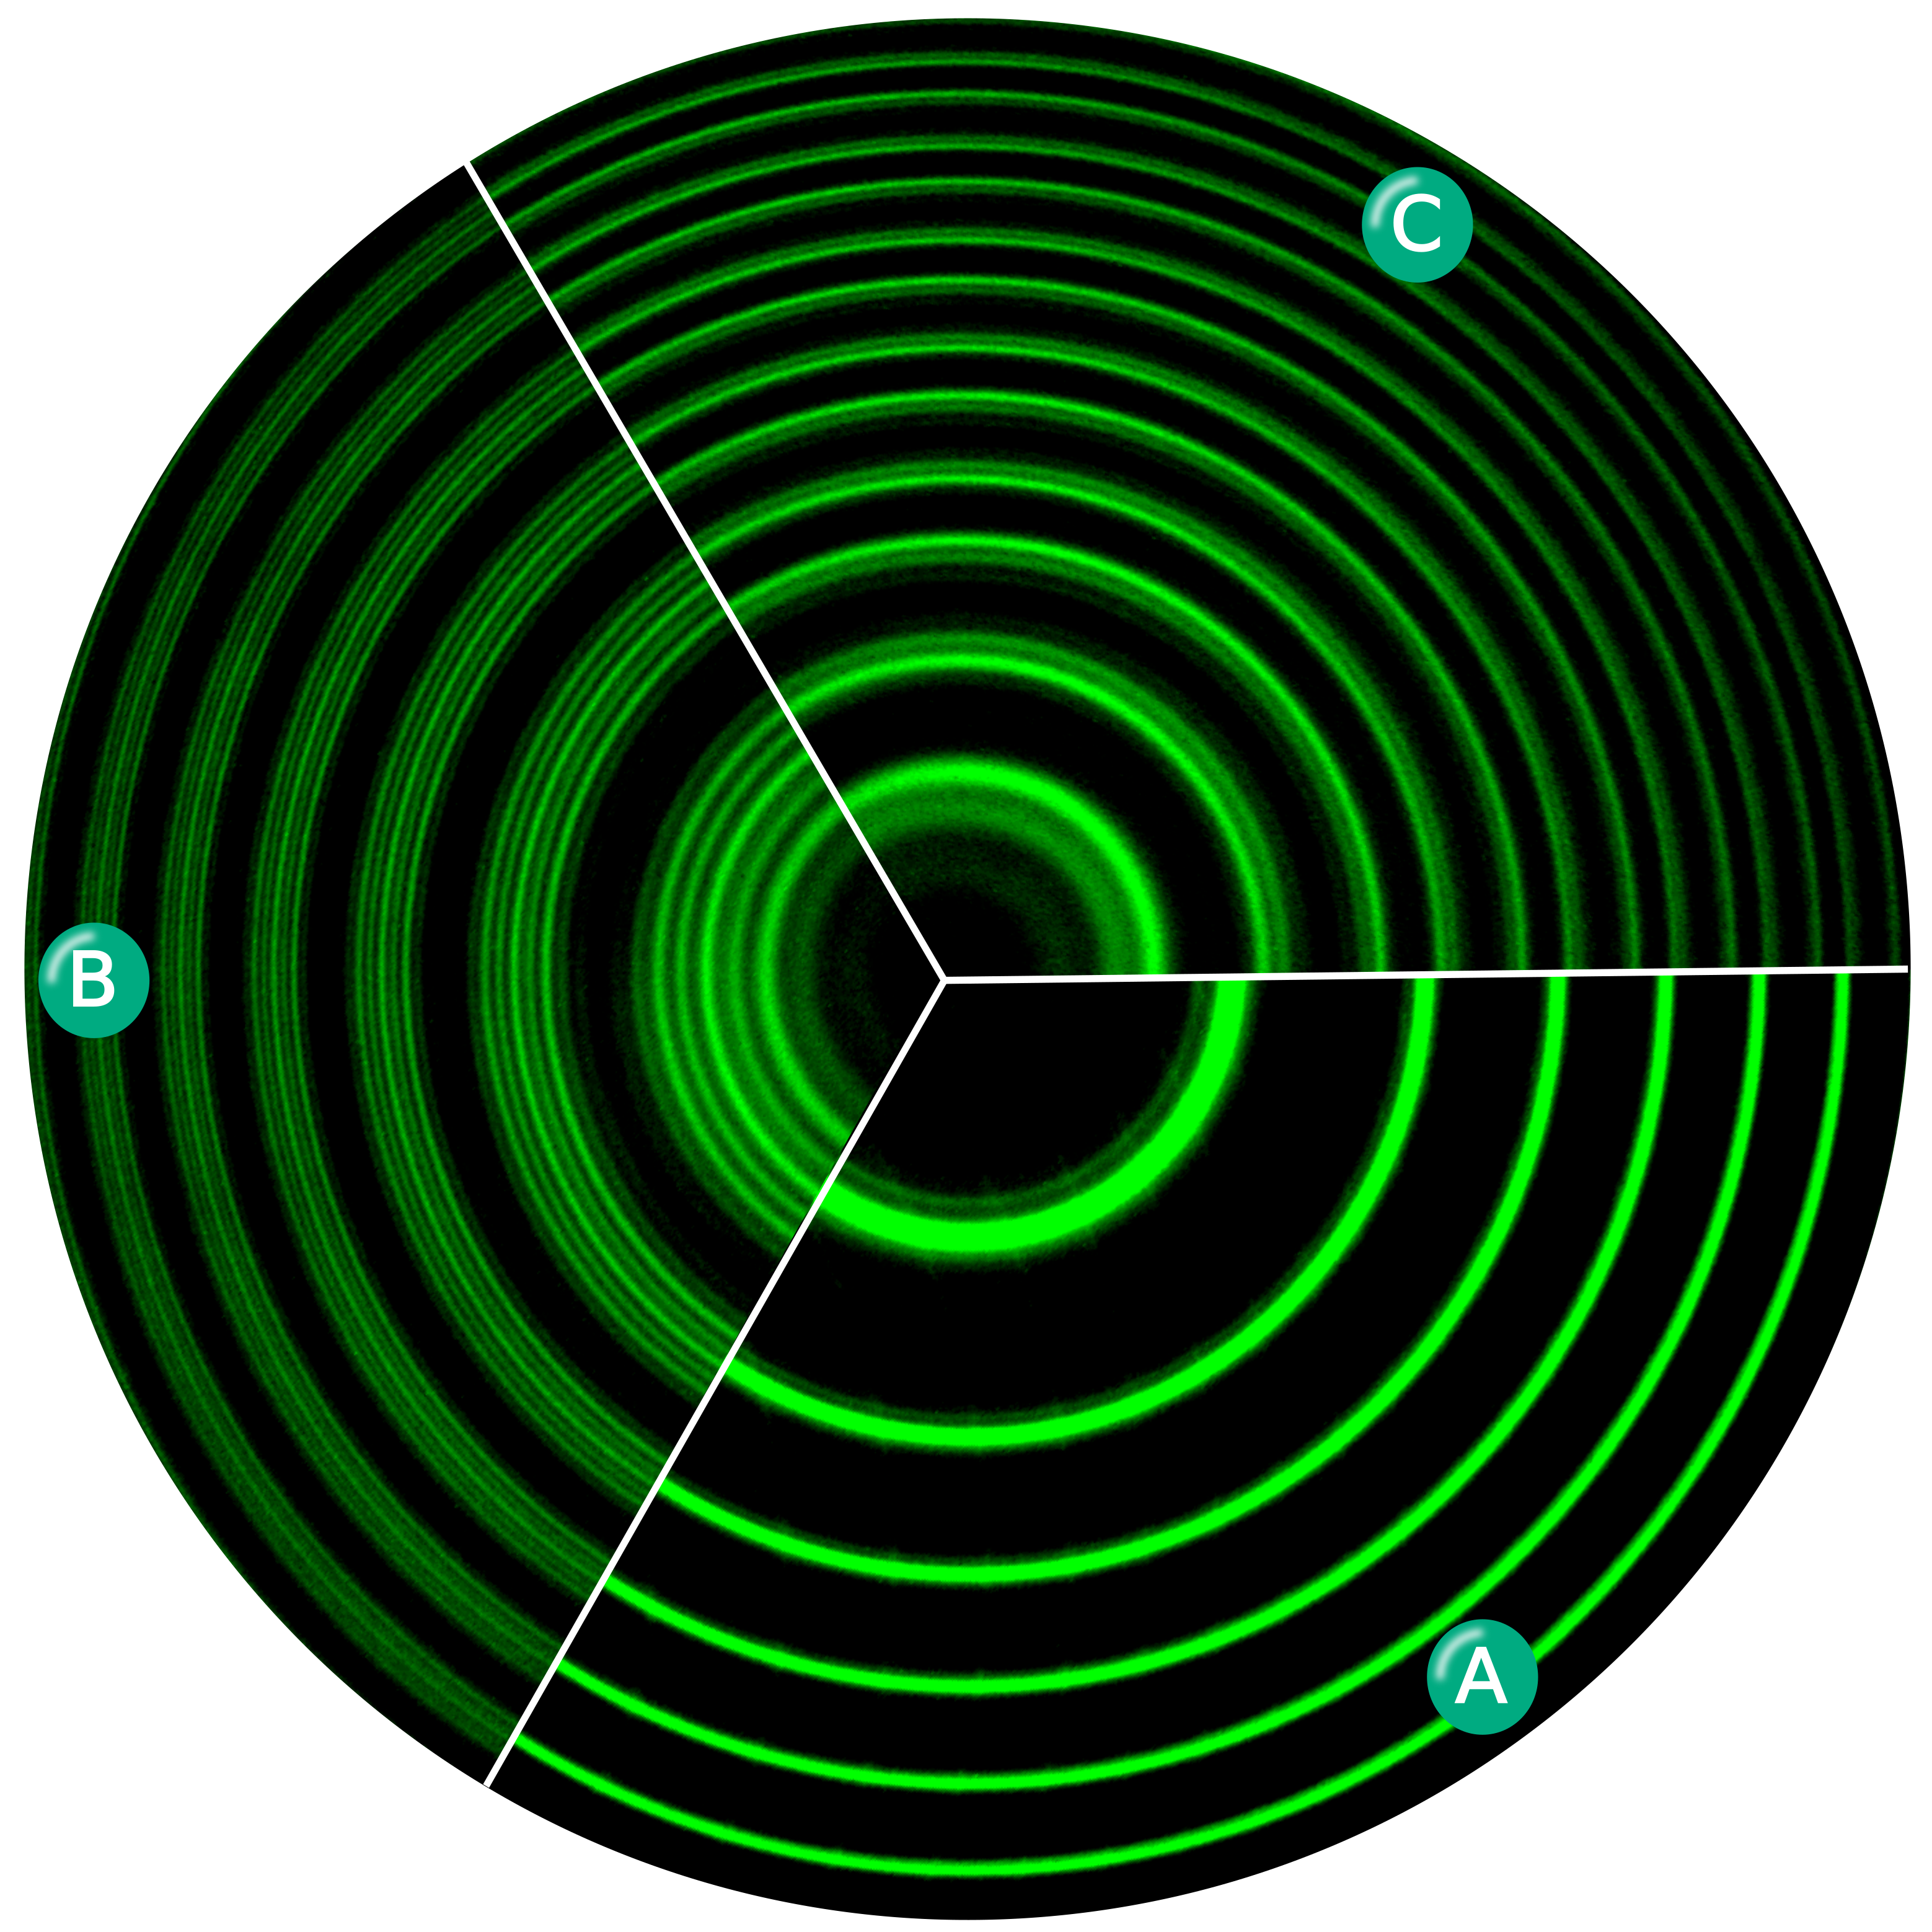
\includegraphics[height=5cm]{fig/chapt2/ZeemanEffectIllus.png}
			\caption{\label{fig:spin:A}}
		\end{subfigure}
		\begin{subfigure}{\linewidth}
			\centering
			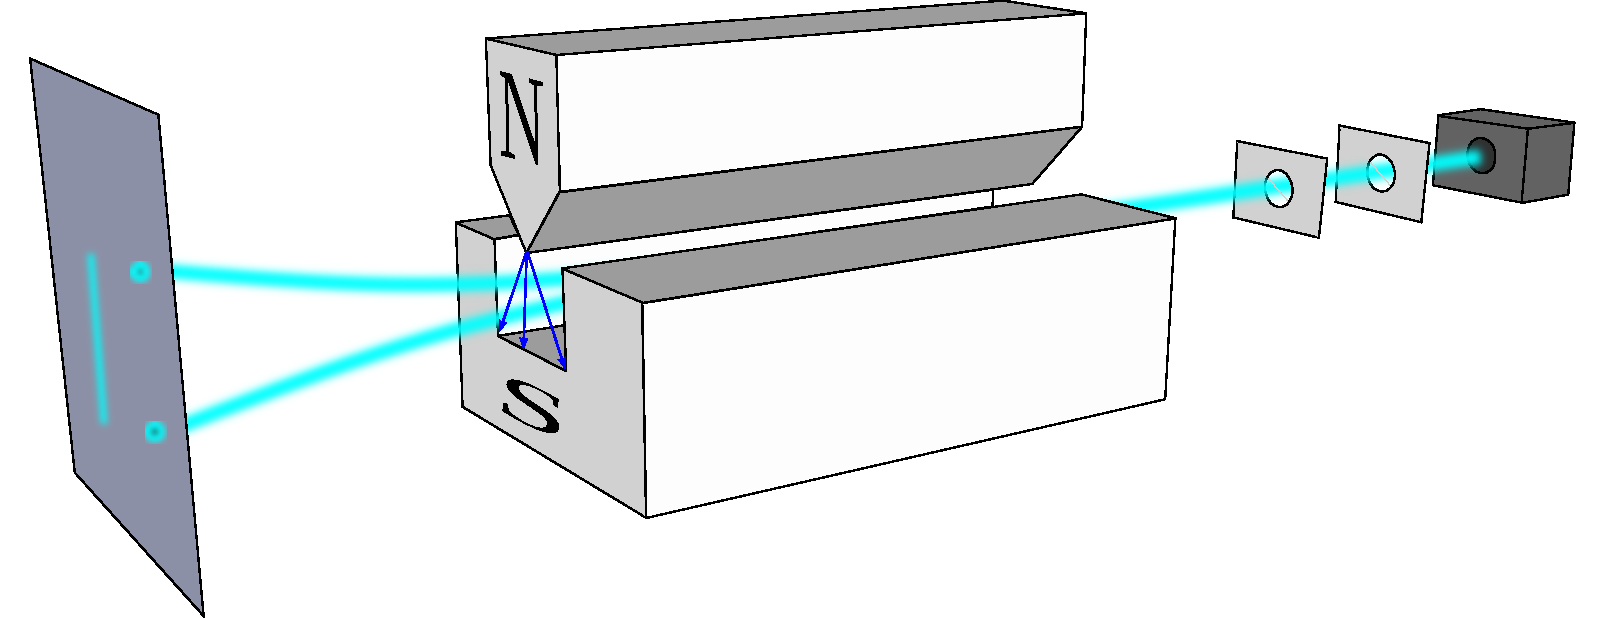
\includegraphics[width = \plotwidth]{fig/chapt2/Stern-Gerlach_experiment.pdf}
			\caption{\label{fig:spin:B}}
		\end{subfigure}
		\caption{\label{fig:spin} Figure~\ref{fig:spin:A}: The spectral lines of mercury vapor lamp anomalous Zeeman effect without magnetic field (A) and with magnetic field (B - transverse Zeeman effect \& C - longitudinal Zeeman effect). Figure~\ref{fig:spin:B}: Stern–Gerlach experiment: Silver atoms traveling through an inhomogeneous magnetic field and being deflected up or down depending on their spin.}
	\end{figure}
	
	Although the intuition of De Broglie about the wave-particle duality of all matter was a step in the right direction, his interpretation was semiclassical and it is in 1926 that the first full quantum wave equation would be introduced by Schrödinger to describe electron-like particles, reproducing the previous semiclassical formulation without inconsistencies~\cite{SCHRODINGER1926}. This complex equation describes the evolution of the wave function $\Psi$ of the quantum system, defined by its position vector $\mathbf{r}$ and time $t$ as an energy conservation law, in which the hamiltonian of the system $\hat{H}$ is explicit, by solving the Equation~\ref{eq:schrodinger}.
	
	\begin{equation}
		\label{eq:schrodinger}
		i\hbar \frac{\partial}{\partial t} \vert \Psi(\mathbf{r},t)\rangle  = \hat{H} \vert \Psi(\mathbf{r},t)\rangle
	\end{equation}
	
	The spin was then included into Schrödinger equation by Pauli to take into account the interaction with an external magnetic field, as shown in Equation~\ref{eq:pauli} in which the Hamiltonian operator is a $2 \times 2$ matrix operator due to the Pauli matrices~\cite{PAULI1927}. $\mathbf{A}$ is the vector potential and $\phi$ is the scalar electric potential.
	
	\begin{equation}
		\label{eq:pauli}
		i\hbar \frac{\partial}{\partial t} \vert\Psi\rangle  =  \left[\frac{1}{2m}(\mathbf{\sigma}\cdot(\mathbf{p}-q\mathbf{A})^2+q\phi)\right]\vert\Psi\rangle
	\end{equation}
	
	Later in 1927, Dirac went further in his paper about emission and absorption of radiation by proposing a second quantization not only of the physical process at play but also of the electromagnetic field~\cite{DIRAC1927}. His equation provided the ingredients to the first formulation of \textit{\acf{QED}} and the description of photon emission by electrons dropping into a lower energy state in which the final number of particles is different than the initial one. Nevertheless, in order to properly treat electromagnetism, the incorporation of the special relativity developed by Einstein was necessary. Derived in 1928, the Dirac equation, shown as Equation~\ref{eq:dirac}, similarly to Schrödinger equation, is a single-particle equation but it incorporates special relativity in addition to quantum mechanics rules~\cite{DIRAC1928}.
	
	\begin{equation}
		\label{eq:dirac}
		i\hbar \gamma^\mu\partial_\mu\psi - mc\psi = 0
	\end{equation}
	
	It features the $4 \times 4$ gamma matrices $\gamma^\mu$ built using $2 \times 2$ Pauli matrices and the unitary matrix, the 4-gradient $\partial_\mu$, the rest mass $m$ of any half integer spin massive particle described by the wave function $\psi(x,t)$, also called a Dirac spinor and the speed of light $c$. In addition to perfectly reproduce the results obtained with quantum mechanics so far, it also provided \textit{negative-energy solutions} that would later be interpreted as a new form of matter, \textit{antimatter}~\cite{OPPENHEIMER1930I,DIRAC1931}. In the non-relativistic limit, the Dirac equation gives a theoretical justification to the Pauli equation that was phenomenologically constructed to account for the spin.
	
	The successes of the QED were soon followed with theoretical problems as computations of any physical process involving photons and charged particles were shown to be only reliable at the first order of the \textit{perturbation theory}~\cite{OPPENHEIMER1930II}. At higher order of the theory, divergent contributions were appearing giving nonsensical results. Only two effects were contributing to these infinities.
	
	\begin{itemize}
		\item The self-energy of the electron (or positron), the energy that the particle has due to its own interaction with its environment.
		\item The vacuum polarization, virtual electron–positron pairs produced by a background electromagnetic field in the vacuum which is not an "empty" space. These virtual pairs affect the charge and current distributions generated by the original electromagnetic field.
	\end{itemize}
	
	Solving this apparent problem was done by carefully defining the concepts of each observable, for example mass or charge, as these quantities are understood within the context of a non-interacting field equation. From the experimental point of view, they are abstractions as what is measured is "renormalized observables" shifted from their "bare" value by the interaction taking place in the measuring process. The infinities needed to be connected to corrections of mass and charge as those are fixed to finite values by experiment. This was the intuition of Bethe in 1947 who successfully computed the effect of such \textit{renormalization} in the non-relativistic case~\cite{BETHE1947}. Full covariant formulations of QED including renormalization were achieved by 1949 by Tomonaga, Schwinger, Feynman, and Dyson~\cite{DYSON1949}. With the resolution of infinities, QED had mostly reached its final form, being still today the most accurate physical theory, and would serve as a model to build all other quantum field theories.
	
	\subsubsection*{Development of the quark model and \acl{QCD}}
	\label{chapt2:sssec:quark}
	
\begingroup\setlength{\intextsep}{0pt}\setlength{\columnsep}{15pt}
	
	\begin{wrapfigure}{r}{0.45\linewidth}
		\begin{minipage}{\linewidth}
			\centering\captionsetup[subfigure]{justification=centering}
			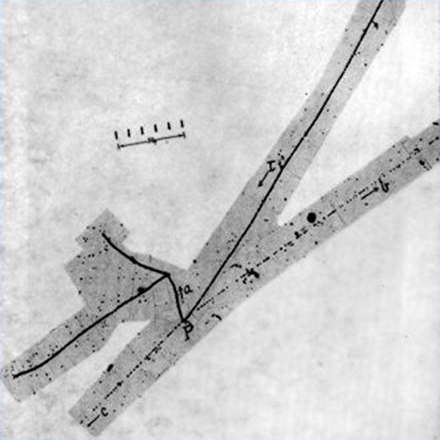
\includegraphics[width=.8\linewidth]{fig/chapt2/mu-meson.png}
			\subcaption{\label{fig:emulsions:A}}
			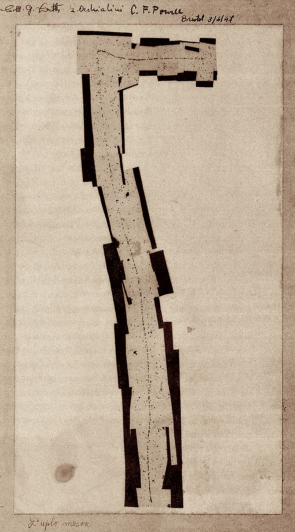
\includegraphics[width=.8\linewidth]{fig/chapt2/pion-emulsion.pdf}
			\subcaption{\label{fig:emulsions:B}}
		\end{minipage}
		\caption{\label{fig:emulsions} Figure~\ref{fig:emulsions:A}: decay of a $\mu$-meson in an emulsion. Figure~\ref{fig:emulsions:B}: track of a $\pi$-meson in an emulsion signed by Lattes, Powell, and Occhialini.}
		\vspace{-5pt}
	\end{wrapfigure}
	
	To explain the nuclear force that holds \textit{nucleons} (protons and neutrons) together, Yukawa proposed in 1934 the existence of a force carrier called \textit{meson} due to its predicted mass in the range in between the electron and nucleon masses~\cite{YUKAWA1935}. Discovered in 1936 by Anderson and Neddermeyer~\cite{ANDERSON1936,NEDDERMEYER1937}, and confirmed using bubble chambers in 1937 by Street and Stevenson~\cite{STREET1937}, a first meson candidate was observed in the decay products of cosmic rays. Assuming it had the same electric charge as electrons and protons, this particle was observed to have a curvature due to magnetic field that was sharper than protons but smoother than electrons resulting in a mass in between the two. But its properties were not compatible with Yukawa's theory, which was emphasized by the discovery of a new candidate in 1947, again in cosmic ray products using photographic emulsions~\cite{LATTES1947I,LATTES1947II,LATTES1947III}. The detections of the mu-meson and of the pi-meson in emulsions are showed in Figure~\ref{fig:emulsions}.
	
	This new candidate, although it had a similar mass than the already believed \textit{meson}, would rather decay into it. For distinction, the first candidate would then be renamed "\textit{mu meson}" when the second would be the "\textit{pi meson}". The \textit{mu meson} was behaving like a heavy electron and didn't participate in the strong interaction whereas the pion was believed to be the carrier of the nuclear interaction. This led to classify the \textit{mu} in a new category of particles  that shared similar properties called \textit{leptons} under the name of \textit{muon} together with the electron. The \textit{pi meson} was finally found to be a triplet of particles: a positively charged, a negatively charged, and a neutral particle. The neutral \textit{pi meson} has been more difficult to identify as it wouldn't leave tracks on emulsions nor on bubble chambers and needed to be studied via its decay products. It was ultimately identified in University of California's cyclotron in 1950 through the observation of its decay into 2 photons~\cite{BJORKLUND1950}.
	
\endgroup
	
	Also discovered in 1947 but in cloud chamber photographs, the \textit{K meson} has also been an important step towards the establishment of the \acl{SM}~\cite{ROCHESTER1947}. A triplet of particles, two charged and a neutral, with a mass roughly half that of a proton, were reported. These particles were baptised \textit{K meson} in contrast to the "light" \textit{pi} and \textit{mu} "L-mesons". The particularity of the \textit{K} is their very slow decays with a typical lifetime of the order of \Ord{-10}\si{s} much longer than the \Ord{-23}\si{s} of \textit{pi}-proton reactions. The concept of \textit{strangeness}, a new quantum number was then introduced thanks to an idea of Pais as an attempt to explain this phenomenon as \textit{strange} particles appeared as the pair production of a strange and anti-strange particle~\cite{PAIS1952}.
	
\begingroup\setlength{\intextsep}{5pt}\setlength{\columnsep}{15pt}
	
	\begin{wrapfigure}{r}{.45\linewidth}
		\vspace{-10pt}
		\begin{minipage}{\linewidth}
			\centering\captionsetup[subfigure]{justification=centering}
			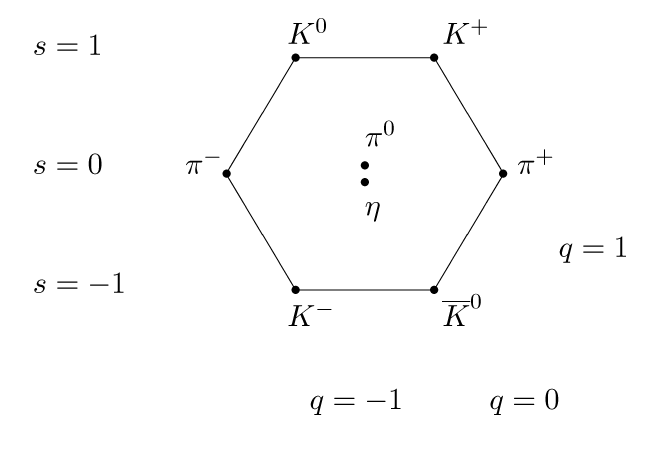
\includegraphics[width=\linewidth]{fig/chapt2/Meson_octet.png}
			\subcaption{\label{fig:Eightfold:A}}
			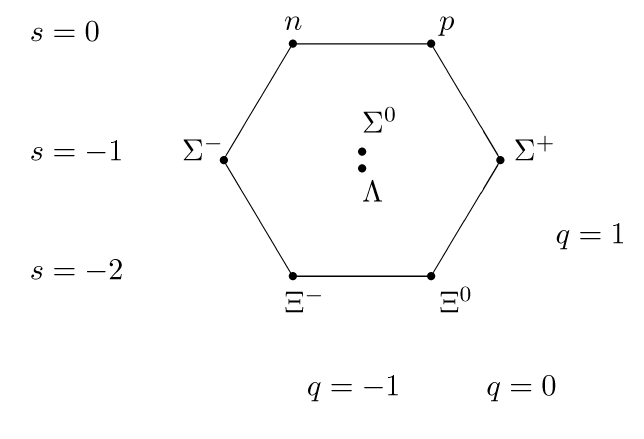
\includegraphics[width=\linewidth]{fig/chapt2/Baryon_octet.png}
			\subcaption{\label{fig:Eightfold:B}}
			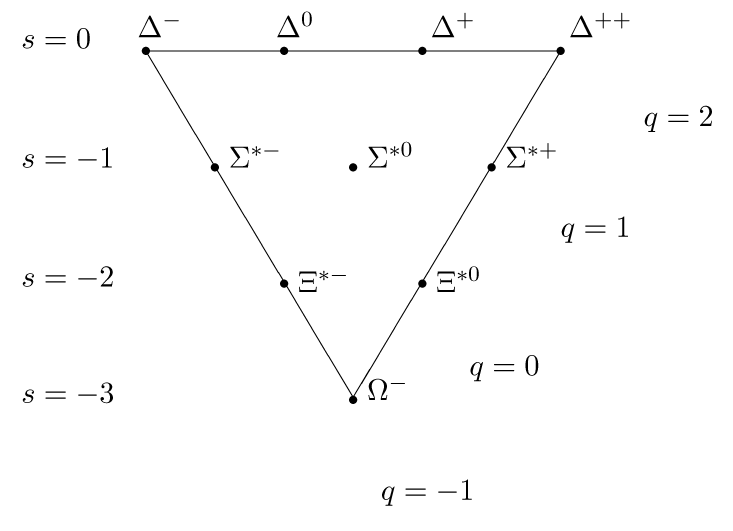
\includegraphics[width=\linewidth]{fig/chapt2/Baryon_decuplet.png}
			\subcaption{\label{fig:Eightfold:C}}
		\end{minipage}
		\caption{\label{fig:Eightfold} Figure~\ref{fig:Eightfold:A}: Meson octet. Figure~\ref{fig:Eightfold:B}: Baryon octet. Figure~\ref{fig:Eightfold:C}: Baryon decuplet.}
		\vspace{-5pt}
	\end{wrapfigure}
	
	With the development of synchrotrons, the particle \textit{zoo} grew to several dozens during the 1950s as higher energies were reachable through acceleration. In 1961, a first classification system, called \textit{Eightfold Way}, was proposed by Gell-Mann~\cite{GELLMANN1962}. It found its roots in the Gell-Mann--Nishijima formula, which relates the electric charge $Q$, the third component of the isospin $I_3$, the \textit{baryon} number $B$ and the strangeness $S$, as showed in Formula~\ref{eq:NNG}~\cite{NISHIJIMA1953,NISHIJIMA1955,GELLMANN1956}.
	
	\begin{equation}
		\label{eq:NNG}
		Q = I_3 + \frac{1}{2}(B+S)
	\end{equation}
	
	The isospin is a quantum number introduced in 1932 to explain symmetries of the newly discovered neutron using representation theory of SU(2)~\cite{HEISENBERG1932}. The baryon number, was introduced by Nishijima as a quantum number for baryons, i.e. particles of the same family as nucleons~\cite{NISHIJIMA1953}. The mesons were classified in an octet and baryons of spin $\pm\frac{1}{2}$ and $\pm\frac{3}{2}$ were respectively classified into an octet and a decuplet, as shown in Figure~\ref{fig:Eightfold}. To complete the baryon decuplet, Gell-Mann predicted the existence of baryon $\Omega^-$ which would later be discovered in 1964~\cite{BARNES1964}.
	
	Gell-Mann, and independently Zweig, then proposed a full theoretical model in which \textit{hadrons} (strongly interacting particles, i.e. mesons and baryons) were not elementary particles anymore~\cite{GELLMANN1964,ZWEIG1964I,ZWEIG1964II}. They were rather composed of three flavors of particles called \textit{quarks} and their anti-particles. The three flavors were called \textit{up}, \textit{down} and \textit{strange}. \textit{Up} and \textit{down} were used to explain the nucleons and non-strange mesons, while \textit{strange} came into the composition of hadrons showing strangeness. \textit{Up} and \textit{down} flavors were discovered in 1968 thanks to the deep inelastic scattering experiments conducted at the \acf{SLAC}~\cite{BLOOM1969,BREIDENBACH1969}, and \textit{strange} could only be indirectly validated even though it provided a robust explanation to \textit{kaon} (K) and \textit{pion} ($\pi$).
	
\endgroup
	
	However, in the decade following the Gell-Mann-Zweig quark model proposition, several improvement to the model were brought. First by Glashow and Bjorken the same year that predicted the existence of a fourth quark flavor, the \textit{charm}, that would equalize the then known number of quarks and leptons~\cite{BJORKEN1964,GLASHOW1970}. Finally in 1973 by Kobayashi and Maskawa that increased the number of quarks to six to explain the experimental observation of CP violation~\cite{CHRISTENSON1964,KOBAYASHI1973}. These two quarks were referred to as \textit{top} and \textit{bottom} for the first time in 1975~\cite{HARARI1975}. It's only after these additions to the quark model that finally the \textit{charm} was discovered in 1974 at both SLAC and \acf{BNL}~\cite{RICHTER1974,TING1974}. A meson in which the \textit{charm} is bonded with an \textit{anti-charm}, called $J/\psi$ and presented in Figure~\ref{fig:JPsi}, helped convince the physics community of the validity of the model. The \textit{bottom} was discovered soon after in 1977 in Fermilab~\cite{HERB1977} and indicated the existence of the \textit{top} that resisted to discovery until Fermilab's experiments CDF and D$\emptyset$ in 1995 due its very large mass and the energy needed to produce it~\cite{ABASHI1995,ABE1995}.
	
	\begin{figure}[H]
		\begin{subfigure}{0.5\linewidth}
			\centering
			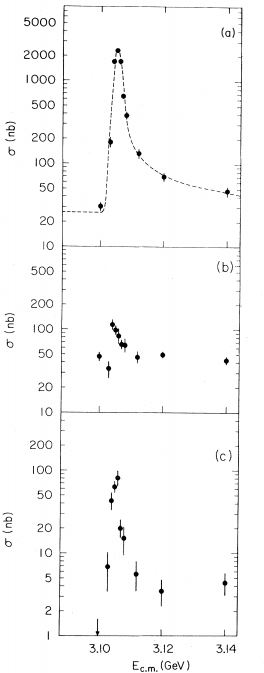
\includegraphics[width=5cm]{fig/chapt2/JPsi-discovery-SPEAR.png}
			\caption{\label{fig:JPsi:A}}
		\end{subfigure}
		\begin{subfigure}{0.5\linewidth}
			\centering
			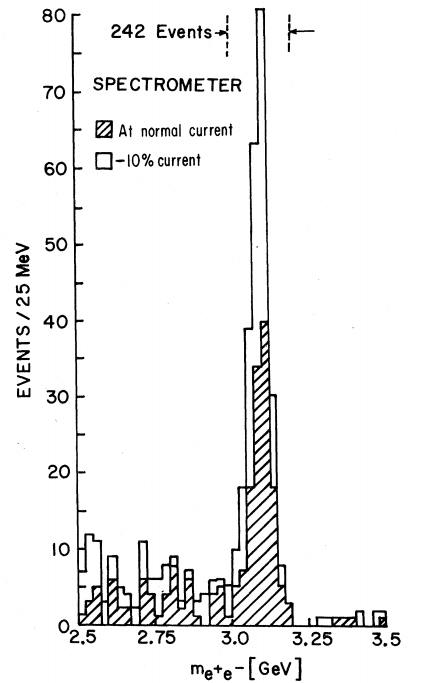
\includegraphics[width=5cm]{fig/chapt2/JPsi-discovery-AGS.png}
			\caption{\label{fig:JPsi:B}}
		\end{subfigure}
		\caption{\label{fig:JPsi} Discovery of the $J/\Psi$ by both SPEAR (SLAC~\cite{RICHTER1974}) in Figure~\ref{fig:JPsi:A} and AGS (BNL~\cite{TING1974}) in Figure~\ref{fig:JPsi:B}. In Figure~\ref{fig:JPsi:A}, the cross section versus energy is showed for (a) multi hadron final states, (b) $e^+e^-$ final states, and (c) $\mu^+\mu^-$, $\pi^+\pi^-$ and $K^+K^-$ final states.}
	\end{figure}
	
	As remarked by Struminsky, due to mesons such as $\Omega^-$ or $\Delta^{++}$, the first SU(3) model already should have possessed an additional quantum number~\cite{STRUMINSKY1965}. Indeed, these mesons are composed of three identical quarks, respectively three \textit{strange} and \textit{up} quarks, with parallel spins, which should be forbidden by the exclusion principle. Independently, Greenberg, and Han and Nambu proposed an additional SU(3) degree of freedom for the quarks~\cite{GREENBERG1964,HANNAMBU1965}. It was later referred to as \textit{color charge gauge}, that could interact through \textit{gluons}, the gauge boson octet corresponding to this degree of freedom. The color field is presented in Figure~\ref{fig:QCD:A}. Nevertheless, as observing free quarks to prove their existence proved to be impossible, two visions of the quarks were argued. On one side, Gell-Mann proposed to see quarks as mathematical construct instead of real particles, as they are always confined, implying that quantum field theory would not describe entirely the strong interaction. He promoted the S-matrix approach to treat the strong interaction. Opposed to this vision, Feynman on the contrary argued that quarks are real particles, that he would call \textit{partons}, that should be described as all other particles by a distribution of position and momentum~\cite{FEYNMAN1969}. The implications of quarks as point-like particles were verified at SLAC and helped abandon the S-matrix to the benefit of QFT~\cite{BJORKEN1969}. The concept of \textit{color} was then added to the quark model in 1973 by Fritzsch and Leutwyler together with Gell-Mann to propose a description of the strong interaction through the theory of \acf{QCD}~\cite{FRITZSCH1973}. The discovery the same year of asymptotic freedom within the QCD by Gross, Politzer, and Wilczek, allowed for very precise predictions thanks to perturbation theory~\cite{GROSS1973,POLITZER1973}. The evolution of the gauge constant of QCD with respect to the energy as described by asymptotic freedom is showed in Figure~\ref{fig:QCD:B}.
	
	\begin{figure}[H]
		\begin{subfigure}{0.6\linewidth}
			\centering
			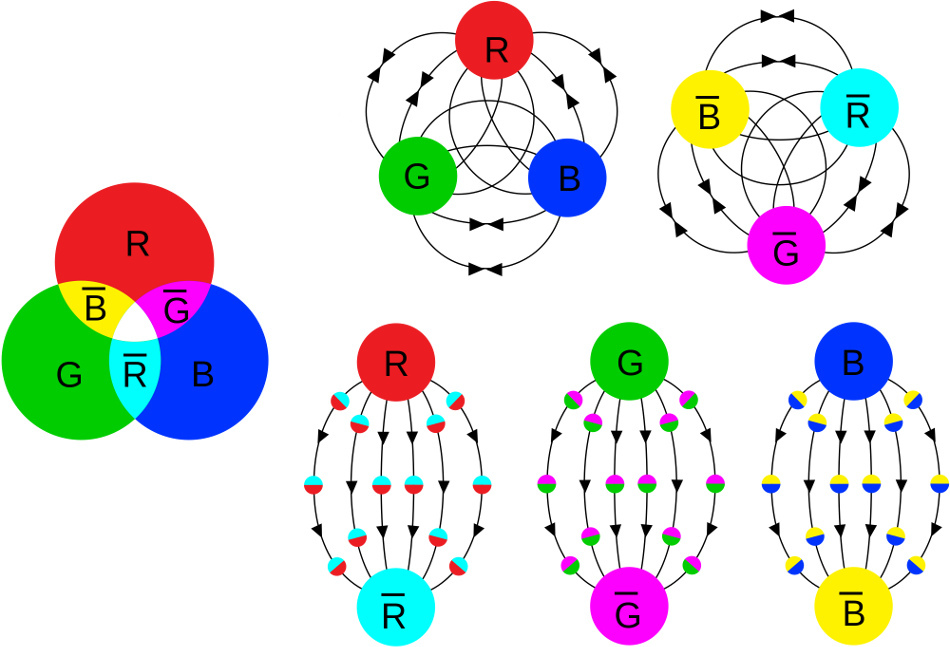
\includegraphics[width=0.7\plotwidth]{fig/chapt2/QCD-colour-field.jpg}
			\caption{\label{fig:QCD:A}}
		\end{subfigure}
		\begin{subfigure}{0.4\linewidth}
			\centering
			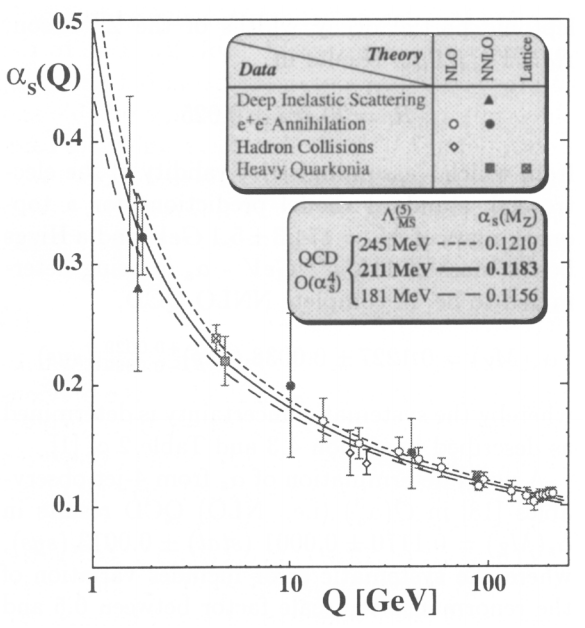
\includegraphics[width=0.5\plotwidth]{fig/chapt2/QCD-asymptotic-freedom.png}
			\caption{\label{fig:QCD:B}}
		\end{subfigure}
		\caption{\label{fig:QCD} Figure~\ref{fig:QCD:A}: the color field of QCD only allows for "white" \textit{baryons}, particles composed of quarks, to exist. Examples are given for mesons, composed of a quark and its anti-quark, and hadrons, composed of three differently colored quarks or anti-quarks. Other exotic baryons have been predicted and observed, such as tetraquarks and pentaquarks. Figure~\ref{fig:QCD:B}: a crossed analysis performed thanks to the data collected by various experiments at different energies have showed that the coupling constant evolves as predicted by the mechanism of asymptotic freedom~\cite{BETHKE2003}.}
	\end{figure}
	
	\subsubsection*{The Weak interaction, spontaneous symmetry breaking, the Higgs mechanism and the Electroweak unification}
	\label{chapt2:sssec:HiggsEW}
	
	The weak interaction is the process that causes radioactive decays. Thanks to the neutron discovery~\cite{CHADWICK1932}, Fermi could explain in 1934 beta radiations through the beta decay process in which the neutron decays into a proton by emitting an electron~\cite{FERMI1934}. Though the missing energy observed during this process triggered a huge debate about the apparent non-conservation of energy, momentum and spin of the process, Fermi, as Pauli before him~\cite{PAULI1930}, proposed that the missing energy was due to a neutral not yet discovered particle that was then baptised \textit{neutrino}. The impossibility to detect such a particle left some members of the scientific community sceptical, but hints of energy conservation and of the existence of the neutrino were provided by measuring the energy spectrum of electrons emitted through beta decay, as there was a strict limit on their energy, as showed in Figure~\ref{fig:beta-decay}.
	
\begingroup\setlength{\intextsep}{5pt}\setlength{\columnsep}{15pt}
	
	\begin{wrapfigure}{l}{0.6\linewidth}
		\centering
		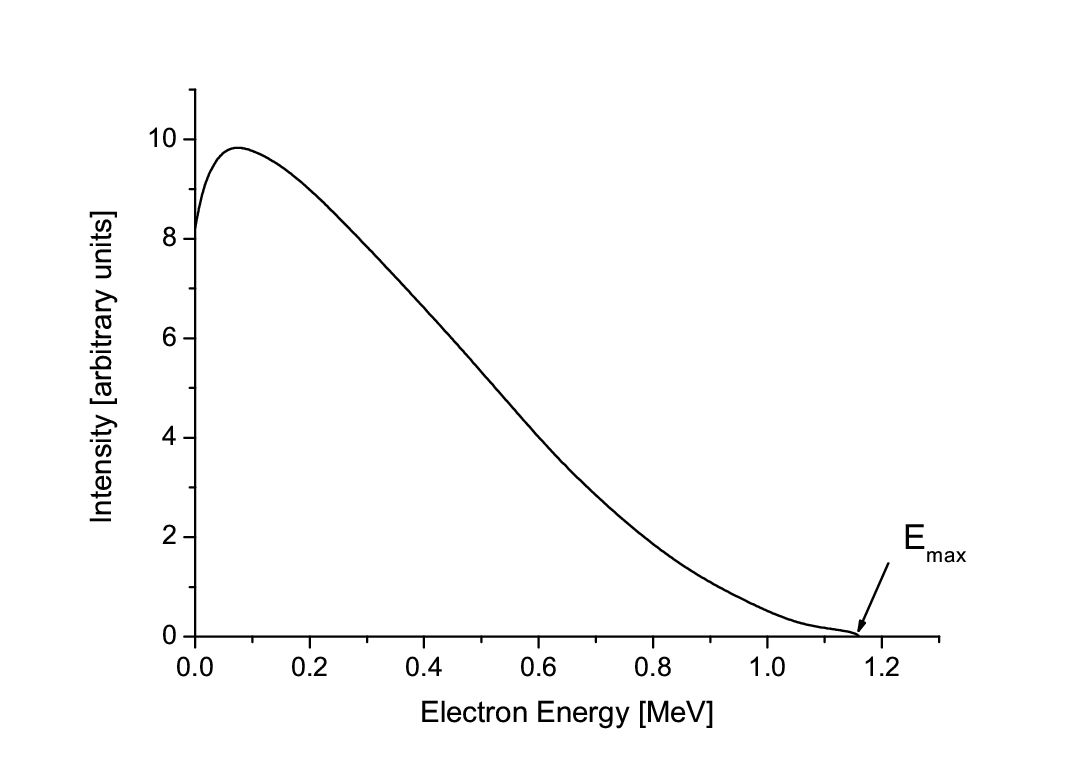
\includegraphics[width=\linewidth]{fig/chapt2/Beta-decay-electron-spectrum.jpg}
		\caption{\label{fig:beta-decay} Energy spectrum of beta particles emitted by a source of $^{210}Bi$.}
	\end{wrapfigure}
	
	It's only 30 years later in 1953 that it was discovered by the team of Cowan and Reines using the principle of inverse beta decay described through Formula~\ref{eq:invbeta}~\cite{COWAN1953}.
	
	\begin{equation}
		\label{eq:invbeta}
		\overline{\nu} + p \rightarrow n + e^+
	\end{equation}
	
	The experiment consisted in placing water tanks sandwiched in between liquid scintillators near a nuclear reactor with an estimated neutrino flux of \Sci{5}{13}\siflux. However, in order to explain the absence of some reactions in the experiment of Cowan and Reines and constraint the beta decay theory of Fermi and extend it to the case of the muon, Konopinski and Mahmoud proposed in 1953 that the muon decay would eject a particle similar to the neutrino~\cite{KONOPINSKI1953}. They predicted the existence of a muon neutrino that would be different to the one involved in the beta decay, related to the electron. With this, the idea of \textit{lepton number} arised. The \textit{muon neutrino} was successfully detected in 1962 by Lederman, Schwartz, and Steinberger~\cite{LEDERMAN1962}.
	
\endgroup
	
	The theory could not be valid though as the probability of interaction, called \textit{cross-section}, would have been increasing without limitation with the square of the energy. Fermi had proposed a two vector current coupling but Lee and Yang noted that an axial current could appear and would violate parity~\cite{LEE1956}. Gamov and Teller had already tried to account for such parity violation by describing Fermi's interaction through allowed (parity-violating) and superallowed (parity-conserving) decays~\cite{GAMOW1936}. The Wu experiment in 1956 confirmed the parity violation~\cite{WU1957}, as showed by Figure~\ref{fig:parity-violation}. But the success of QED as a quantum field theory sparked the development of similar theory to describe the weak interaction.
	
	As previously discussed, the great success of QED was built on an underlying symmetry, interpreted as a gauge invariance so that the effect of the force is the same in all space-time coordinates, and of the possibility to renormalize it in order to resolve infinities. In 1967, Weinberg found a way to unite both the electromagnetic and weak interaction into a gauge theory involving four gauge bosons, three of which are massive and carry out the weak interaction and the last is a massless boson carrying the electromagnetic interaction~\cite{WEINBERG1967}. Among the three massive bosons, two are charged and one is neutral, similarly to the previously theorized \textit{pi meson} vector of the Yukawa model~\cite{YUKAWA1935} and all have a mass much greater than nucleons and thus a very short life time implying a finite very short range, contrary to the contact interaction originally proposed by Fermi.
	
	\begin{figure}[H]
		\begin{subfigure}{0.5\linewidth}
			\centering
			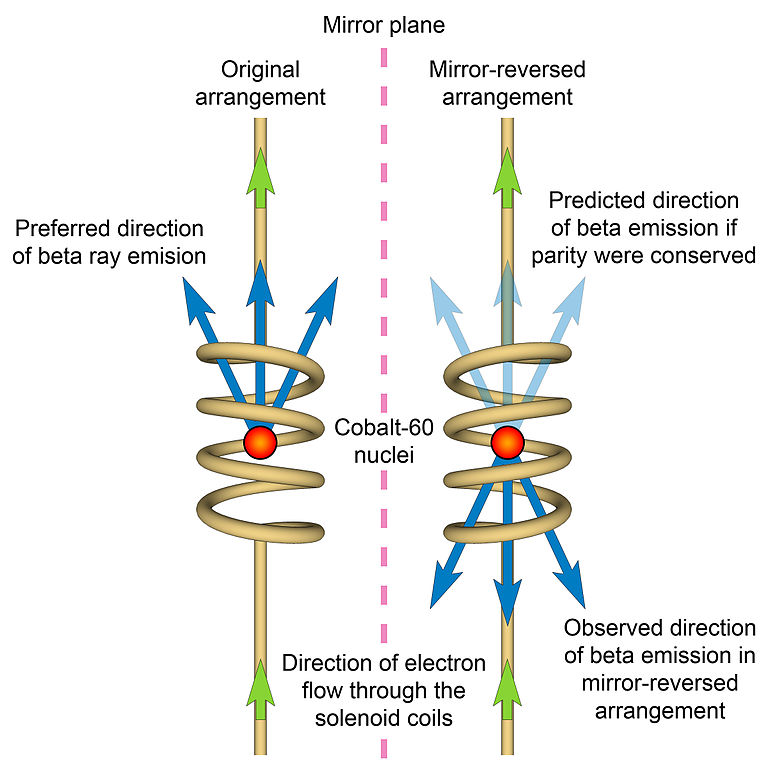
\includegraphics[width=0.6\plotwidth]{fig/chapt2/Wu_experiment.jpg}
			\caption{\label{fig:parity-violation:A}}
		\end{subfigure}
		\begin{subfigure}{0.5\linewidth}
			\centering
			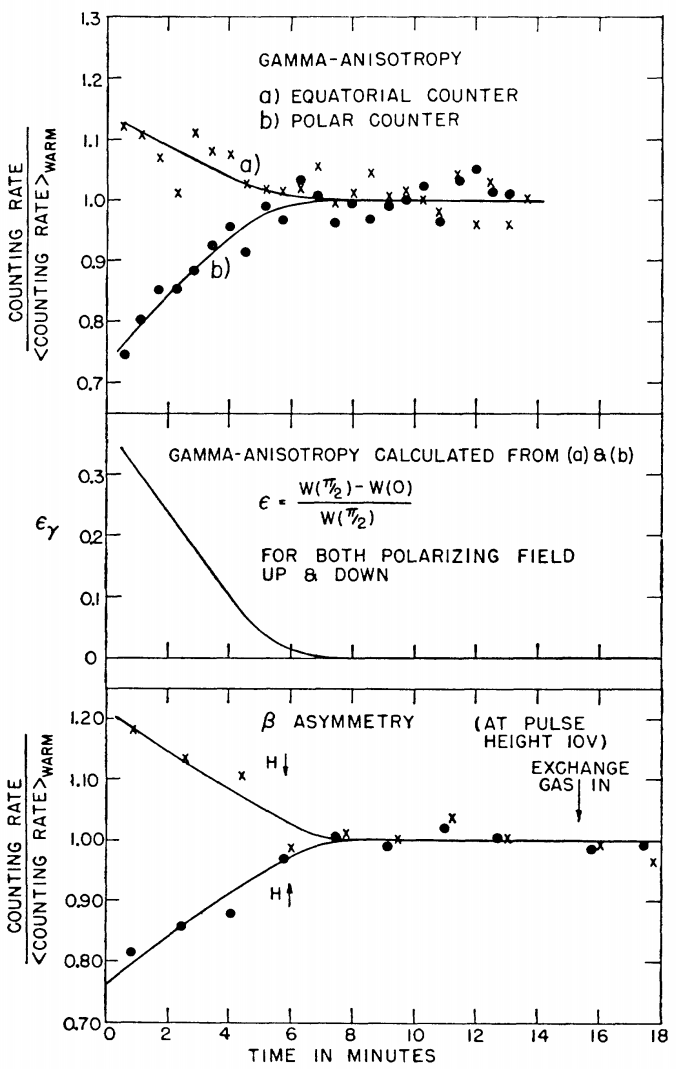
\includegraphics[width=0.5\plotwidth]{fig/chapt2/Wu_result.png}
			\caption{\label{fig:parity-violation:B}}
		\end{subfigure}
		\caption{\label{fig:parity-violation} As explained through Figure~\ref{fig:parity-violation:A}, the Wu experiment consisted in measuring the preferred direction of emission of beta rays of a Colbalt source placed in a stable magnetic field aligned, in one case, and anti-aligned, in the other case, with the nuclear spin. The result of Figure~\ref{fig:parity-violation:B} showed a violation of parity.}
	\end{figure}
	
	Breakthroughs in other fields of physics contributed in giving theoretical support and interpretation to the unified electroweak theory. The stepping stone was the use of spontaneous symmetry breaking that was inspired to Nambu at the beginning of the 1960s~\cite{NAMBU1961I,NAMBU1961II} following the development of the \acf{BCS} superconductivity mechanism in 1957~\cite{BCS1957}. Cooper had shown that BCS pairs, pairs of electrons bound together at low temperature, can have lower energy than the Fermi Energy and are responsible for superconductivity. This led to the discovery of Goldstone-Nambu bosons~\cite{NAMBU1960,GOLDSTONE1961} as a result of the spontaneous breaking of the chiral symmetry in a theory describing nucleons and mesons developed by Nambu and Jona-Lasinio in 1961, and now understood as a low-energy approximation of QCD. Similarly to the mechanism of energy gap appearance in superconductivity, the nucleon mass is suggested to be the result of a self-energy of a fermion field and is studied through a four-fermion interaction in which, as a consequence of the symmetry, bound states of nucleon-antinucleon pairs appear and can be regarded as virtual pions. Though the symmetry is maintained in the equations, the ground state is not preserved. Goldstone showed that the bound states correspond to spinless bosons with zero mass~\cite{GOLDSTONE1961}.
	
	Although the model in itself didn't revolutionize particle physics, spontaneous symmetry breaking was generalized to quantum field theories. As all fundamental interactions are described using gauge theories based on underlying symmetries, processes such as the chiral symmetry breaking were introduced soon after the publication of Nambu and Jona-Lasinio. In 1962, Anderson, discussed the implications of spontaneous symmetry breaking in particles physics~\cite{ANDERSON1963}. He did so by following the idea of Schwinger who suggested that zero-mass vector bosons were not necessarily required to describe the conservation of baryons, contrary to the bosons emerging from chiral symmetry breaking~\cite{SCHWINGER1962}. A model was finally independently built in 1964 by Brout and Englert~\cite{ENGLERT1964}, Higgs~\cite{HIGGS1964}, and Guralnik, Hagen, and Kibble~\cite{GURALNIK1964}, who discovered that combining an additional field into a gauge theory in order to break the symmetry, the resulting gauge bosons acquire a nonzero mass. Moreover, Higgs stated that this implied the existence of at least one new massive, i.e. self-interacting, scalar boson corresponding to this additional field, that is now known as \textit{Higgs boson}. The Higgs mechanism today specifically refers to the process through which the gauge bosons of the weak interaction acquire mass. In 1967, Weinberg could point to the Higgs mechanism to integrate a Higgs field into a new version of the electroweak theory in which the spontaneous symmetry breaking mechanism of the Higgs field would explicitly explain the masses of the weak interaction gauge bosons and the zero-mass of photons~\cite{WEINBERG1967}.
	
	\subsection{Construction and validation of the \acl{SM}}
	\label{chapt2:ssec:model}
	
	The Standard Model of particle physics was built in the middle of the 1970s after the experimental confirmation of the existence of quarks~\cite{SMWIKI}. It is based on the assembly of the models previously introduced and describing the fundamental interactions and their gauge bosons, except for gravitation, as well as the way elementary "matter" particles interact with the fields associated with these force carriers. In this sense, the development of QED and the unification of the electroweak interaction, of the Yukawa interaction and of QCD, and of the Higg mechanism made it possible to explain most of the contemporary physics.
	
	In the SM, "matter" particles, are described by twelve fermion fields of spin $\frac{1}{2}$ obeying the Fermi-Dirac statistics, i.e. subjected to the Pauli exclusion principle. To each fermion is associated its corresponding anti-particle. The fermions are classified according to the way they interact and thus according to the charges they carry. Six of them are classified as quarks ($u$, $d$, $c$, $s$, $t$, and $b$) and are subjected to all interactions and the six others as leptons ($e^-$, $\mu^-$, $\tau^-$, $\nu_e$, $\nu_\mu$, and $\nu_\tau$). Leptons are not subjected to the strong interaction and among them, the three neutrinos only interact weakly as they are neutral particles, which explains why they are so difficult to detect. The gauge boson fields are the gluons $g$ for the strong interaction, the photon $\gamma$ for the electromagnetic interaction and the weak bosons $W^+$, $W^-$, and $Z^0$ for the weak interaction. Finally, the Higgs field $H^0$ is responsible, through the spontaneous symmetry breaking, of the mixing of the massless electroweak boson fields $W_1$, $W_2$, $W_3$, and $B$ leading to the observable states $\gamma$, $W^+$, $W^-$, and $Z^0$ that can gain mass while interacting with the Higgs field. This picture of the SM is summarized through Figure~\ref{fig:SM} where the antifermions are not shown.
	
	When the model was first finalized, the existence of the weak gauge bosons, of the charm, of the third quark generation composed of top and bottom quarks to explain the observed CP violation was not proven but the predictions were measured with good precision in the years following~\cite{TING1974,RICHTER1974,HERB1977,ABASHI1995,ABE1995}. The weak bosons W and Z were discovered during the next decade in 1983~\cite{UA1W1983,UA2W1983,UA1Z1983,UA2Z1983}. The very last predicted elementary particle of the model that was not observed yet proved to be very difficult to observe. The Higgs boson needed the start of the LHC to finally be observed in 2012~\cite{ATLAS2012,CMS2012}. A few years more of tests were necessary to measure its properties to confirm the observation of a scalar boson compatible with the predicted Higgs boson $H^0$~\cite{HIGGS2015}.
	
	\begin{figure}[H]
		\centering
		\hspace*{-0.1\linewidth}
		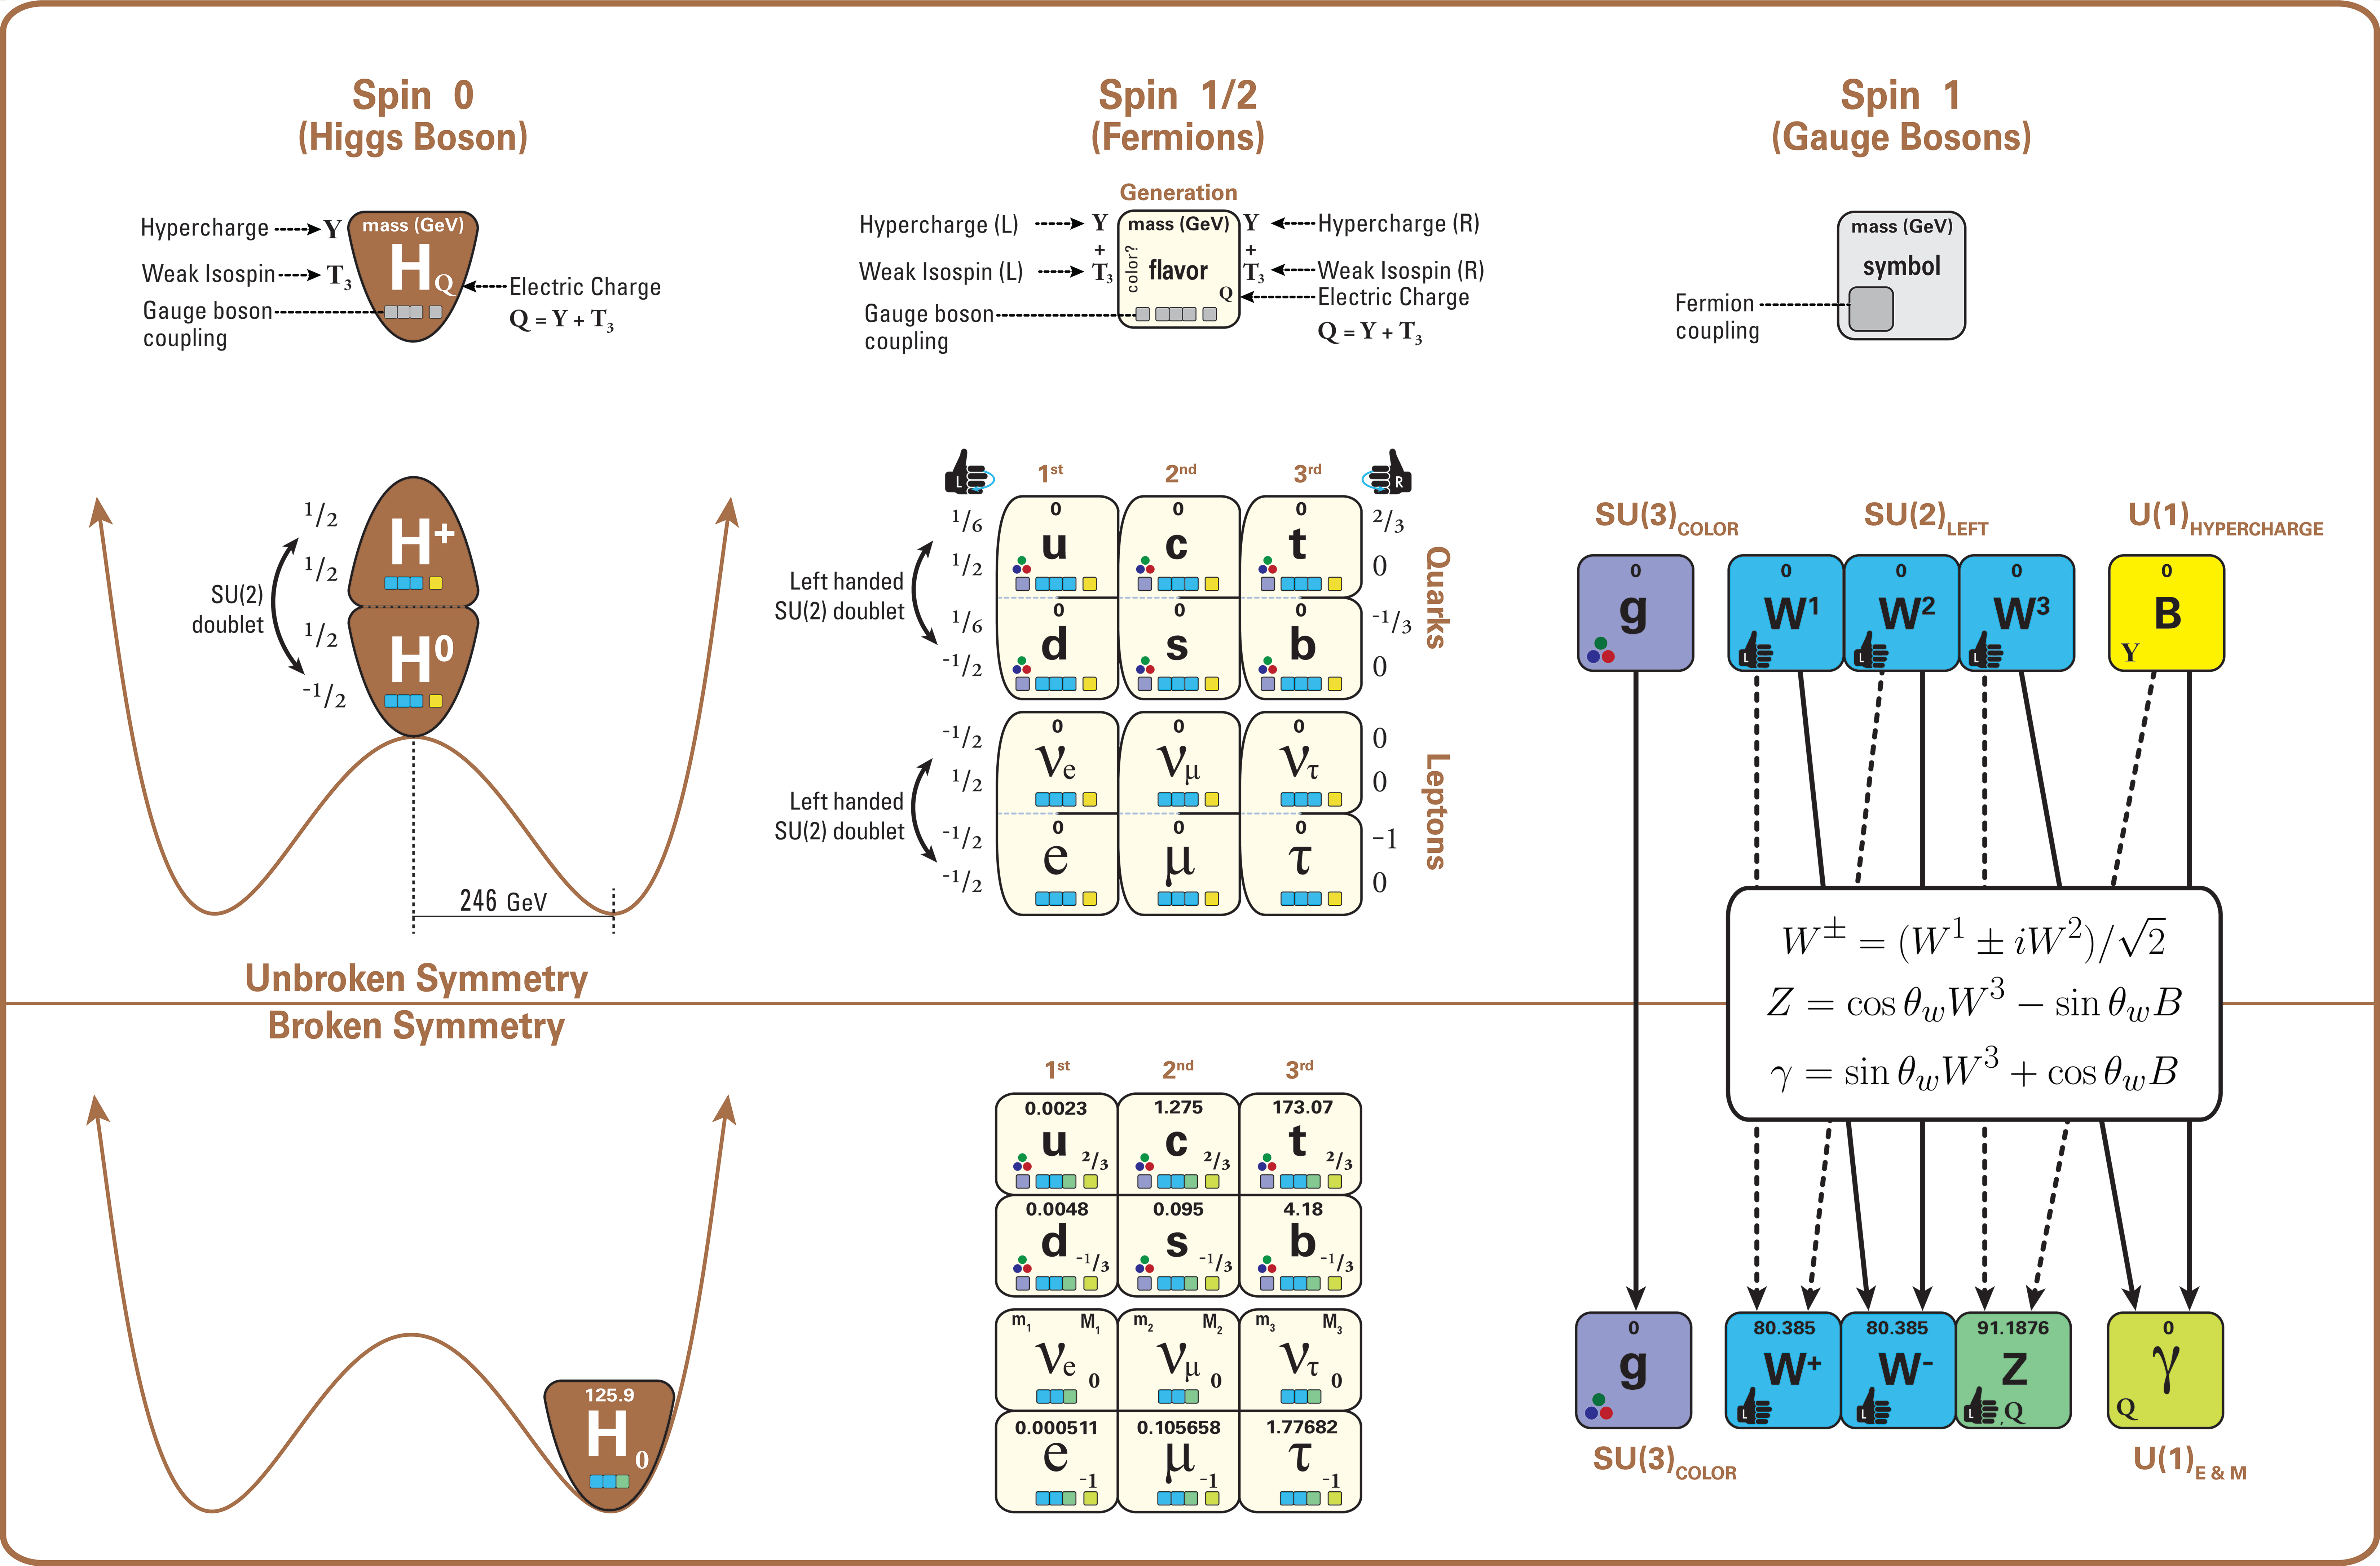
\includegraphics[width=1.2\linewidth]{fig/chapt2/Standard_Model_Of_Particle_Physics.png}
		\caption{\label{fig:SM} The elementary particles of the Standard Model are shown along with their properties. Their interactions with the strong, weak and electromagnetic forces have been made explicit using color squares. In the left column, the scalar Higgs boson is depicted. The center is focused on the matter particles, the fermions, and the right column on the force carriers, the gauge bosons. The role of the Higgs boson in electroweak symmetry breaking is highlighted, and the corresponding way properties of the various particles differ in the (high-energy) symmetric phase (top) and the (low-energy) broken-symmetry phase (bottom) are shown.}
	\end{figure}
	
	\subsection{Investigating the TeV scale}
	\label{chapt2:ssec:TeV}
	
	In \acl{HEP}, the number of experimental events depends on the total interaction cross-section of the colliding particles and of the \textit{instantaneous luminosity}~\cite{PDG2018}. The luminosity is a quantity providing an information on the interaction rate normalised to the interaction cross-section. The relationship between number of events $N$, cross-section and instantaneous luminosity $\lum$ is given in Formula ~\ref{eq:luminosity}.
	
	\begin{equation}
		\label{eq:luminosity}
		\lum = \frac{1}{\sigma}\frac{\deriv N}{\deriv t} \Leftrightarrow N = \sigma \int \lum\: \deriv t = \sigma \lum_{int}
	\end{equation}
	
	The integral of the luminosity over time is referred to as the \textit{integrated luminosity} $\lum_{int}$. In fact, the instantaneous luminosity can be deduced from the beam parameters. New colliders now use bunched beams. The instantaneous luminosity then depends on the bunch crossing frequency $f_{BX}$, on the number of particles contained in each bunch $n$, and on the \textsc{rms} transverse beam sizes in the horizontal, $\sigma^*_x$, and vertical directions, $\sigma^*_y$, at the level of the interaction point. The beam sizes  can be assumed to be identical, leading to the relation of Formula~\ref{eq:lumibeam}.
	
	\begin{equation}
		\label{eq:lumibeam}
		\lum = f_{BX}\frac{n^2}{\sigma^*}
	\end{equation}
	
\begingroup\setlength{\intextsep}{0pt}\setlength{\columnsep}{15pt}
	
	\begin{wrapfigure}{r}{.5\linewidth}
		\vspace{15pt}
		\begin{minipage}{\linewidth}
			\centering\captionsetup[subfigure]{justification=centering}
			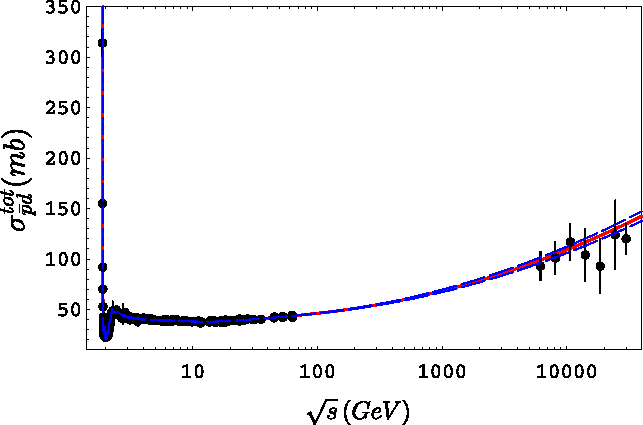
\includegraphics[width=\linewidth]{fig/chapt2/pp-total-cross-section.pdf}
			\subcaption{\label{fig:pp-cross-section:A}}
			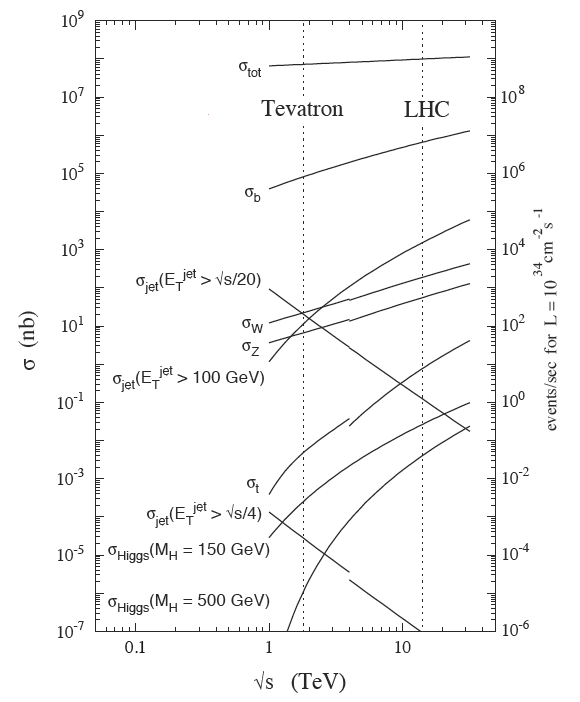
\includegraphics[width=\linewidth]{fig/chapt2/Cross-sections.png}
			\subcaption{\label{fig:pp-cross-section:B}}
		\end{minipage}
		\caption{\label{fig:pp-cross-section} Figure~\ref{fig:pp-cross-section:A}: Total proton-proton cross-section as a function of the collisions center-of-mass energy $\sqrt{s}$~\cite{ARKHIPOV2001} with cosmic-ray data from Akeno Observatory and Fly’s Eye Collaboration. Figure~\ref{fig:pp-cross-section:B}: Total proton-(anti)proton and interaction channel cross-sections in the \si{TeV} scale.}
	\end{wrapfigure}
	
	This expression doesn't depend on time anymore and leads to a simple estimation of the integrated luminosity and hence, knowing the cross-section of each available physics channel, to the expected number of events in each channel. The total interaction cross section is the sum of all the different output channels allowed by the interaction process. In the case of highly relativistic protons, the proton-proton (pp) total cross-section increases with the center-of-mass energy of interactions, as can be seen from Figure~\ref{fig:pp-cross-section}.
	
	Enhancing rare processes that allow to finely test the \acl{SM} is then achieved through an increase in both energy and luminosity. At the energy range that were scanned thanks to high-energy colliders, the SM has so far been a well tested theory. Nevertheless, several hints of physics going beyond its scope have been observed.
	
	\paragraph*{Dark matter and gravity: }
	
	The discrepancy of velocity dispersion of stars in galaxies with respect to the visible mass they contain is known since the end of the \Th{19} century where Kelvin proposed that this problem could be solved if a great majority of the stars would be dark bodies, idea strongly criticized by Pointcaré~\cite{POINTCARE1906}. Throughout the \Th{20} century, physicists like Kapteyn~\cite{KAPTEYN1922} or Zwicky~\cite{ZWICKY1933,ZWICKY1937}, showed the first hints of a \textit{dark matter} by studying star velocities and galactic clusters, followed by robust measurements of galaxy rotation curves by Babcock which suggested that the mass-to-luminosity ratio was different from what would be expected from watching the visible light~\cite{BABCOCK1939}. Later in the 1970s, Rubin and Ford from direct light observations~\cite{RUNBIN1970} and Rogstad and Shostak from radio measurements~\cite{ROGSTAD1972} showed that the radial velocity of visible objects in galaxies was increasing with increasing distance to the center of the galaxy. An example of galaxy rotation curve is provided in Figure~\ref{fig:galaxy}. Finally observation of lensing effect by galaxy clusters, temperature distribution of hot gas in galaxies and clusters, and the anisotropies in the \acf{CMB}, showed in Figure~\ref{fig:CMB}, kept on pointing to a \textit{dark matter}~\cite{PLANK2016}. From all the data accumulated, the visible matter would only account to no more than 5\% of the total content on the visible universe~\cite{JAROSIK2011}. Alternative theories have tried to investigate modified versions of the General Relativity as this theory is only well tested at the scale of the solar system but is not sufficiently tested on wider ranges or even theories in which gravitation is not a fundamental force but rather an emergent one~\cite{VERLINDE2016,MAEDER2017}. But so far, such theories have difficulties to reproduce all the experimental observations as easily as through dark matter.

\endgroup
	
\begingroup\setlength{\intextsep}{0pt}\setlength{\columnsep}{15pt}
	
	\begin{wrapfigure}{l}{.6\linewidth}
		\centering
		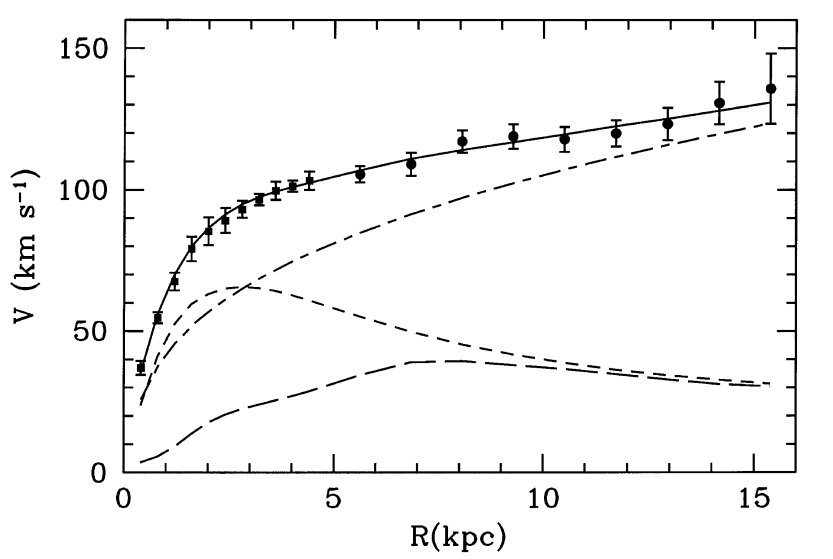
\includegraphics[width=\linewidth]{fig/chapt2/M33-rotation-curve.png}
		\caption{\label{fig:galaxy} Rotation curve (points) of the galaxy M33 compared with best fitting model (line). The short-dashed line represents the rotation profile that would be expected from the observation of the stellar disc alone~\cite{CORBELLI2000}.}
	\end{wrapfigure}
	
	A possible theory to offer dark matter candidates would be \textit{supersymmetry} (SUSY) which proposes a relationship in between bosons and fermions in the frame of the \acf{MSSM}. In this model, each elementary particle, through a spontaneous space-time symmetry breaking mechanism would have a \textit{super partner} from the other family of particles, pairing bosons and fermions together. The model was first introduced as a way to solve the \textit{Hierarchy Problem}~\cite{DIMOPOULOS1981}. The discrepancy between the strength of the weak force and gravity translates into a light Higgs boson compared to the \textit{Planck Mass}. In the SM, the Higgs mass is left to be a measured parameter rather than a calculated one even though the model requires a mass in between 100 and \SI{1000}{GeV/c^2} to stay unitary. Nevertheless, quantum corrections to the Higgs mass coming from its interactions with virtual particles should make the scalar boson much heavier than what measured~\cite{TANEDO2012}. Through the MSSM, the stability of fermion masses would provide stability to the Higgs boson mass via the introduction of a fermionic super partner.
	
\endgroup
	
	On top of providing a solution to the Hierarchy Problem, the model comes with heavy dark matter candidates in the \si{TeV} scale~\cite{JUNGMAN1996}. Indeed, in the case \textit{R-parity} is not violated, the \acf{LSP} cannot decay and could then explain the dark matter. The LSP in the model is neutral and can only interact through the weak and gravitational interactions. Typical candidates are the \textit{neutralino}, the \textit{sneutrino} or the \textit{gravitino}.
	
	Finally, gravity is not explained through the SM, and huge difficulties are encountered when trying to include it. The strength of gravitational interaction is expected to be negligible at the scale of elementary particles, nevertheless, adding gravitation in the perspective of developing a \textit{"theory of everything"} leads to divergent integrals that could not be fixed through renormalization. Extensions to the MSSM, and in particular \acf{mSUGRA}, include general relativity as mediator of the symmetry breaking. mSUGRA gives access to the hidden sector in which the MSSM only interacts gravitationally and suppresses the infinities arising from attempts to include gravity into the SM thanks to possible renormalization~\cite{CHAMSEDDINE1982}.
	
	Signatures for the MSSM would come from the super partners of quarks and gluons that can decay into an LSP that could then be identified as missing energy as it escapes the detectors undetected. But even in the case MSSM predictions are not to be seen, the other models treating dark matter also propose \acf{WIMPs} that could be observed in similar ways than LSPs~\cite{ASKEW2014}. Moreover alternative models exist to provide solutions to the Hierarchy Problem. The most investigated models are extra dimensions such as Arkani-Hamed Dimopoulos Dvali~\cite{ADD1998,ADD1999}, Kaluza–Klein~\cite{KALUZA1921,KLEIN1926} or Randall-Sundrum models~\cite{RS1999I,RS1999II} that usually also include gravitation. Finally, alternative models also exist for the production of dark matter candidates. Models with a hidden valley that would unravel the existence of a new group of light particles through the extension of the SM with a new confining gauge group~\cite{ZUREK2007}.\\
	
	\begin{figure}[H]
		\centering
		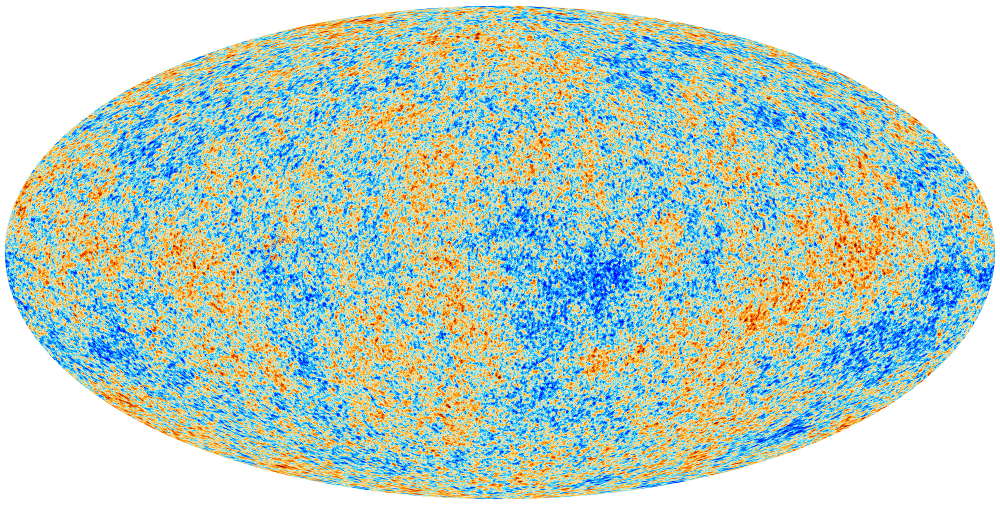
\includegraphics[width=\plotwidth]{fig/chapt2/CMB.jpg}
		\caption{\label{fig:CMB} \acl{CMB} as measured by the space observatory Planck which mean temperature is $T_\gamma =$ \numerror{2.7255}{0.0006}\si{K} with anisotropies of the order of a few \si{\micro K}.}
	\end{figure}
	 
	\paragraph*{Baryon asymmetry: }
	
	Another intriguing fact is that the universe is dominated by matter. However, the SM predicted that matter and antimatter should have been created in equal amounts. For an interaction to produce matter and antimatter at different rates within the SM, three necessary conditions were highlighted by Sakharov\cite{SAKHAROV1967}. First of all, there must be a violation of the baryon number $B$. Then, there must be a C-symmetry and CP-symmetry violation. The C-symmetry violation must happen to make sure that the processes creating more baryons than antibaryons are not compensated by processes creating more anti-baryons and similarly, the CP-symmetry violation makes sure that there are not equal numbers of left-handed baryons and right-handed anti-baryons produced. Finally, the interactions must happen out of thermal equilibrium to make sure that CPT-symmetry does not balance the processes increasing the baryon number with processes doing otherwise~\cite{SHAPOSHNIKOV1993}. An out-of-equilibrium interaction implies a new instable heavy particle.
	
	The favoured model to explain this imbalance is the \textit{baryogenesis} that requires electroweak symmetry breaking to be first order phase transition to fall within the scope of SM~\cite{KUZMIN1985,CANETTI2012}. This means that the symmetry breaking process must involve the absorption or release of a fixed latent heat. Through the baryogenesis, the phase transition breaks P-symmetry spontaneously and allows for CP-symmetry violation. In turn, the CP violation makes the amplitude of interactions involving quarks different than the ones involving anti-quarks leading to the greater creation rate of baryons with respect to anti-baryons. The key to this baryon net creation would be found into the \textit{sphaleron}. A sphaleron is a particle-like saddle point of the energy functional that appears at the top of the transition barrier and that could be created if a sufficiently large amount of energy is brought as the tunneling effect through the barrier is largely suppressed for electroweak interactions. The existence of the sphaleron would allow violation of the conservation of $B$ but also of the leptonic number $L$ while conserving $B-L$. The detection at $p-p$-colliders of such a transition is foreseen to be made through processes with high-multiplicity final states such as $u + u \rightarrow e^+\mu^+\tau^+\bar{t}\bar{t}\bar{b}\bar{c}\bar{c}\bar{s}\bar{d} + X$\cite{CMSSPHALERON2018}. To be probed, the sphaleron transition requires an energy $E_{sph} \approx$ \SI{9}{TeV}. Nevertheless, if such transition cannot be observed, other BSM models such as the WIMP baryogenesis could be then observed thanks to the detection of displaced vertices, featuring the decay of a WIMP leading to violation of $B$~\cite{SHUVE2015}.
	
	Another possibility to explain the apparent asymmetry would be the existence of an \acf{EDM} in any fundamental particle that would permit matter and antimatter particles to decay at different rates~\cite{ACME2014}. Indeed, the presence of an EDM violates in itself both $P$ and $T$ symmetries. Experiments are able to probe for the EDM of various fundamental particles sich as the electron~\cite{ACME2014}, the charm and strange quarks~\cite{NERI2017} or even a heavy neutrino EDM~\cite{STEVENS2018}.\\
	
	\paragraph*{Neutrino mass and sterile neutrino scenario: }
	
	The SM considers neutrinos to be massless. But it was showed in the late 1960s by the Homestake experiment that the flux of solar neutrinos (i.e. $\nu_e$) measured didn't match the predicted values~\cite{DAVIS1968}. The mechanism of neutrino oscillations as a solution to the discrepancy was proposed by Pontecorvo~\cite{PONTECORVO1968} and confirmed in the early 2000s by the Sudbury Neutrino Observatory~\cite{SNO2002}. This oscillation implies that neutrinos that can be observed are a superposition of massive neutrino states. The research on neutrino oscillation is already quite advanced with experiments looking at atmospheric, reactor or beam neutrinos in order to determine the elements of the mixing matrix (Pontecorvo–Maki–Nakagawa–Sakata matrix~\cite{MNS1962}) similar to the \acf{CKM} matrix describing the mixing of quarks~\cite{KOBAYASHI1973}. Nevertheless, no answer to the origin of neutrino mass is yet provided.
	
	Explaining the light non-zero mass of the neutrinos $\nu_l$ ($l = e,\mu,tau$) of the order of the \si{eV} can be done through the Seesaw mechanism~\cite{MINKOWSKI1977,MOHAPATRA1980}. This model features heavy Majorana counterparts $N_l$ ($l = e,\mu,tau$) to the $\nu_l$. The masses of the light and heavy neutrinos are linked through a $2 \times 2$ mass matrix $A$ with eigenvalues $\lambda_{\pm}$ expressed as in Equation~\ref{eq:seesaw}.
	
	\begin{equation}
		\label{eq:seesaw}
		\begin{array}{r c l}
			A & = & \begin{pmatrix}
				0 & M \\
				M & B \\
				\end{pmatrix}\\
			\lambda_{\pm} & = & \frac{B \pm \sqrt{B^2 + 4M^2}}{2}\\
		\end{array}
	\end{equation}
	
	The Majorana mass term $B$ is assumed to be comparable to the Grand Unified Theory scale (\Ord{16} \si{GeV}) while the Dirac mass term $M$ is of the order of electroweak scale (\SI{246}{GeV}). In these conditions, the eigenvalue $\lambda_+$ is almost $B$ while $\lambda_-$ is close to the ratio $-M^2/B$ compatible with very light neutrinos with masses of the order of \SI{1}{eV}. Studying the left-right symmetric model seeking for the parity violation in weak interactions leads to the incorporation of three additional gauge bosons $W_R$ and $Z'$ as a result of the spontaneous symmetry breaking. The processes that are predicted by the model and can be probed at colliders are processes such as $pp \rightarrow W_R \rightarrow l + N_l + X$ and $pp \rightarrow Z' \rightarrow N_l + N_l + X$ where the heavy neutrinos decay as $N_l \rightarrow l + j_1 + j_2$, $j_i$ being jets~\cite{CMSPHYSICSTDR2}. Other version of seesaw mechanisms exist to account for the neutrino mass that can also be explained thanks to supersymmetric models~\cite{VALLE2006}.
	
	%For example, one of LHCb experiment's goal is to investigate CP-violation and thus baryonic asymmetry. In 2017, the collaboration has announced to have so far a \Sig{3.3} statistical significance over a CP-violation through the study of the decays of $\Lambda^0_b$ and $\overline{\Lambda^0_b}$ into a proton (or antiproton) and 3 pions. Many analysis teams are also working hard on supersymmetry both in ATLAS and CMS collaborations, the two multipurpose experiments of LHC, even though no evidence of a supersymmetrical theory was seen, the few hint having the tendency to confirm the standard model. These experiments also have the possibility to investigate ways to explain Majorana neutrino mass through Yukawa interactions of scalar particles.
	
	%The higher the center-of-mass energy, the smaller details the experiments will be able to see, the heavier the potential particle creation barrier will be, the stronger the cross-section of certain rare decay channels will be. As a comparison, with collisions happening at \SI{14}{TeV}, the LHC is approximately 2 orders of magnitude more sensitive to the Higgs than the Tevatron was with its already very powerful \SI{2}{TeV}. All these advantages eventually lead to new discoveries and deeper understanding of the models describing our Universe. But the LHC only is a step forward to gather more precise tests of the Standard Model and new knowledge about the physics beyond it. A successful physics campaign will probably serve to justify the building of new accelerators with even greater discovery potential like for example the \acf{FCC} that would push even further the study of the unanswered questions of contemporary physics.
	
	%Even though only quark-antiquark (mesons) and three quark states (baryons) have been observed, exotic hadrons are not forbidden by QCD and no limit in terms of quark content to form hadrons is imposed by the theory. Moreover, gluons could form bond states by themselves and with quarks. These two types of states are called \textit{glueballs} and \textit{hybrid hadrons}. For decades, experiments have been conducted without confirmation of such possible states existing. Nevertheless, in 2014, tetraquarks were observed by LHCb, one of LHC's main experiments, and in 2015, the same experiment reported the discovery of pentaquarks making the SM one of the best tested theories of physics.

\section{The \acl{LHC} \& the \acl{CMS}}
\label{chapt2:sec:LHC-CMS}

	Throughout its history, CERN has played a leading role in high-energy physics. Large regional facilities such as CERN were planned after the second world war in an attempt to increase international scientific collaboration and to allow scientists to share the forever increasing costs of experimental facilities. Indeed, it is necessary to use always more powerful tools to improve the fine understanding of our Universe. The construction of the first CERN accelerators at the end of the 50s, the \acf{SC} and the \acf{PS}, was directly followed by the first observation of antinuclei in 1965~\cite{MASSAM1965}. The very first proton-proton collider showing hints of protons not being elementary particles was the \acf{ISR}. From this experience, the \acf{SPS} was built in the 70s to investigate the structure of protons, the preference for matter over antimatter, the state of matter in the early universe or exotic particles, and led to the discovery in 1983 of the W and Z bosons~\cite{UA1W1983,UA2W1983,UA1Z1983,UA2Z1983}. These newly discovered particles and the electroweak interaction were then studied in detail by the \acf{LEP} collider that proved that there only are three generations of elementary particles in 1989~\cite{ALEPH1989}. The LEP was then dismantled in 2000 to allow for the LHC to be constructed in the existing tunnel.

	\subsection{LHC, the most powerful particle accelerator}
	\label{chapt2:ssec:LHC}

	\begin{figure}[H]
		\centering
		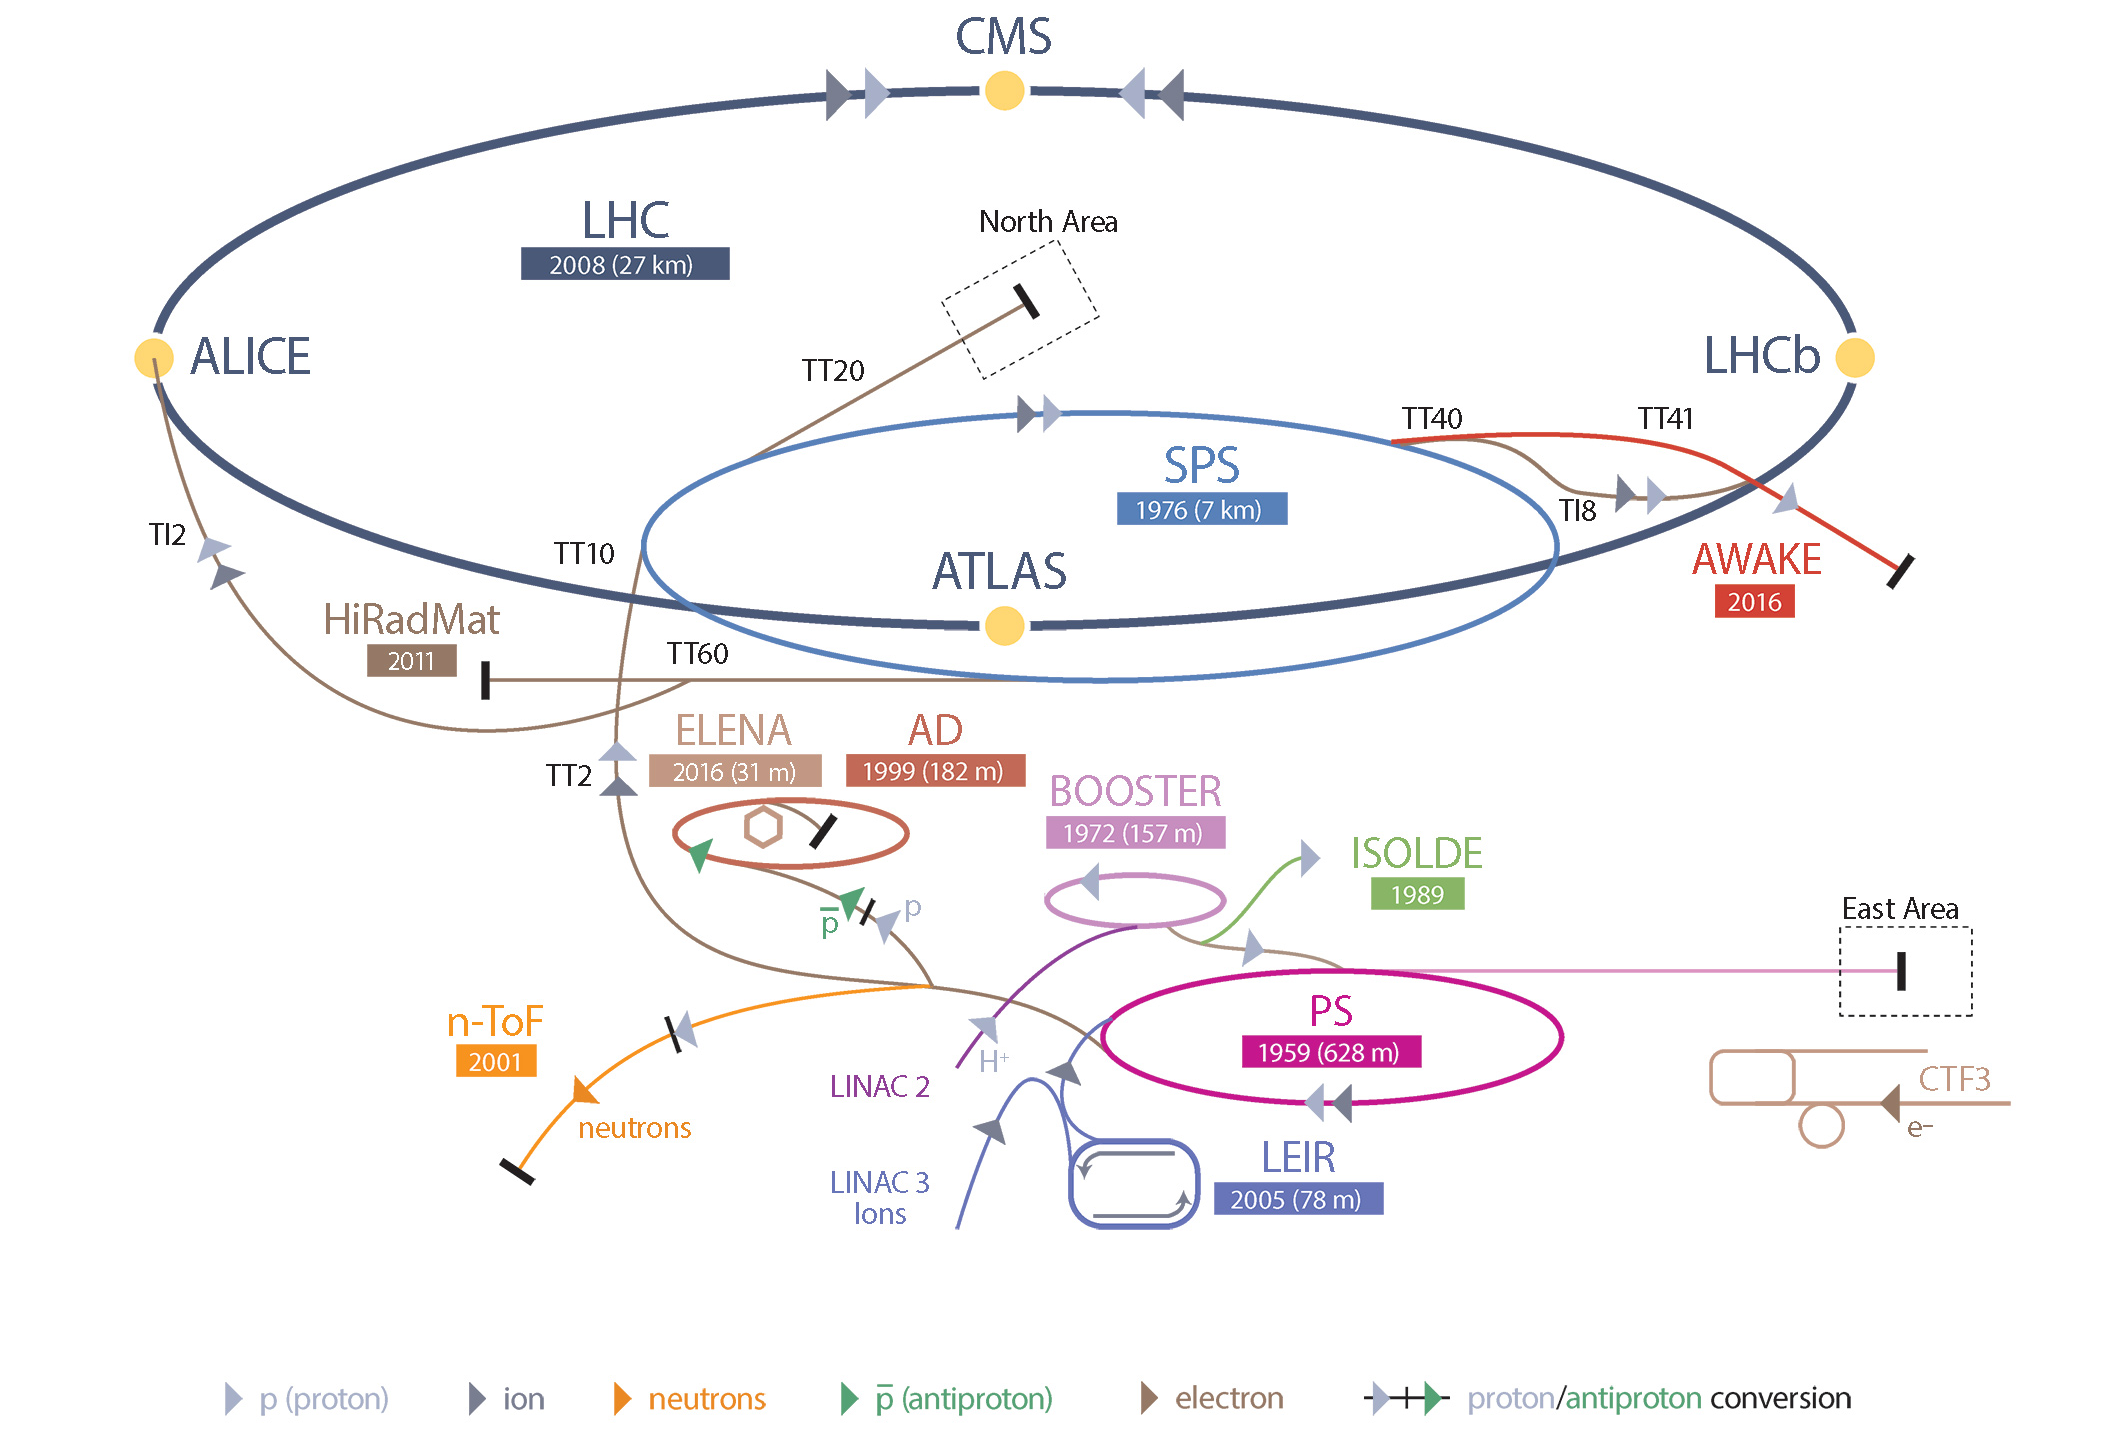
\includegraphics[width=\linewidth]{fig/chapt2/CERN_Accelerator_Complex.png}
		\caption{\label{fig:CERNComplex} CERN accelerator complex.}
	\end{figure}
	
	The different aspects of physics beyond the Standard Model of particle physics and the Standard Model itself can be tested through the use of very energetic and intense hadron and ion colliders. Powerful hadron colliders are suited for searching for strongly interacting particles. The LHC at CERN is a perfect tool to seek answers to these open questions and the experiments build along its beam lines already started investigating further into the SM and BSM physics.
	
\begingroup\setlength{\intextsep}{-15pt}\setlength{\columnsep}{15pt}

	\begin{wrapfigure}{r}{.47\linewidth}
		\centering
		\vspace{15pt}
		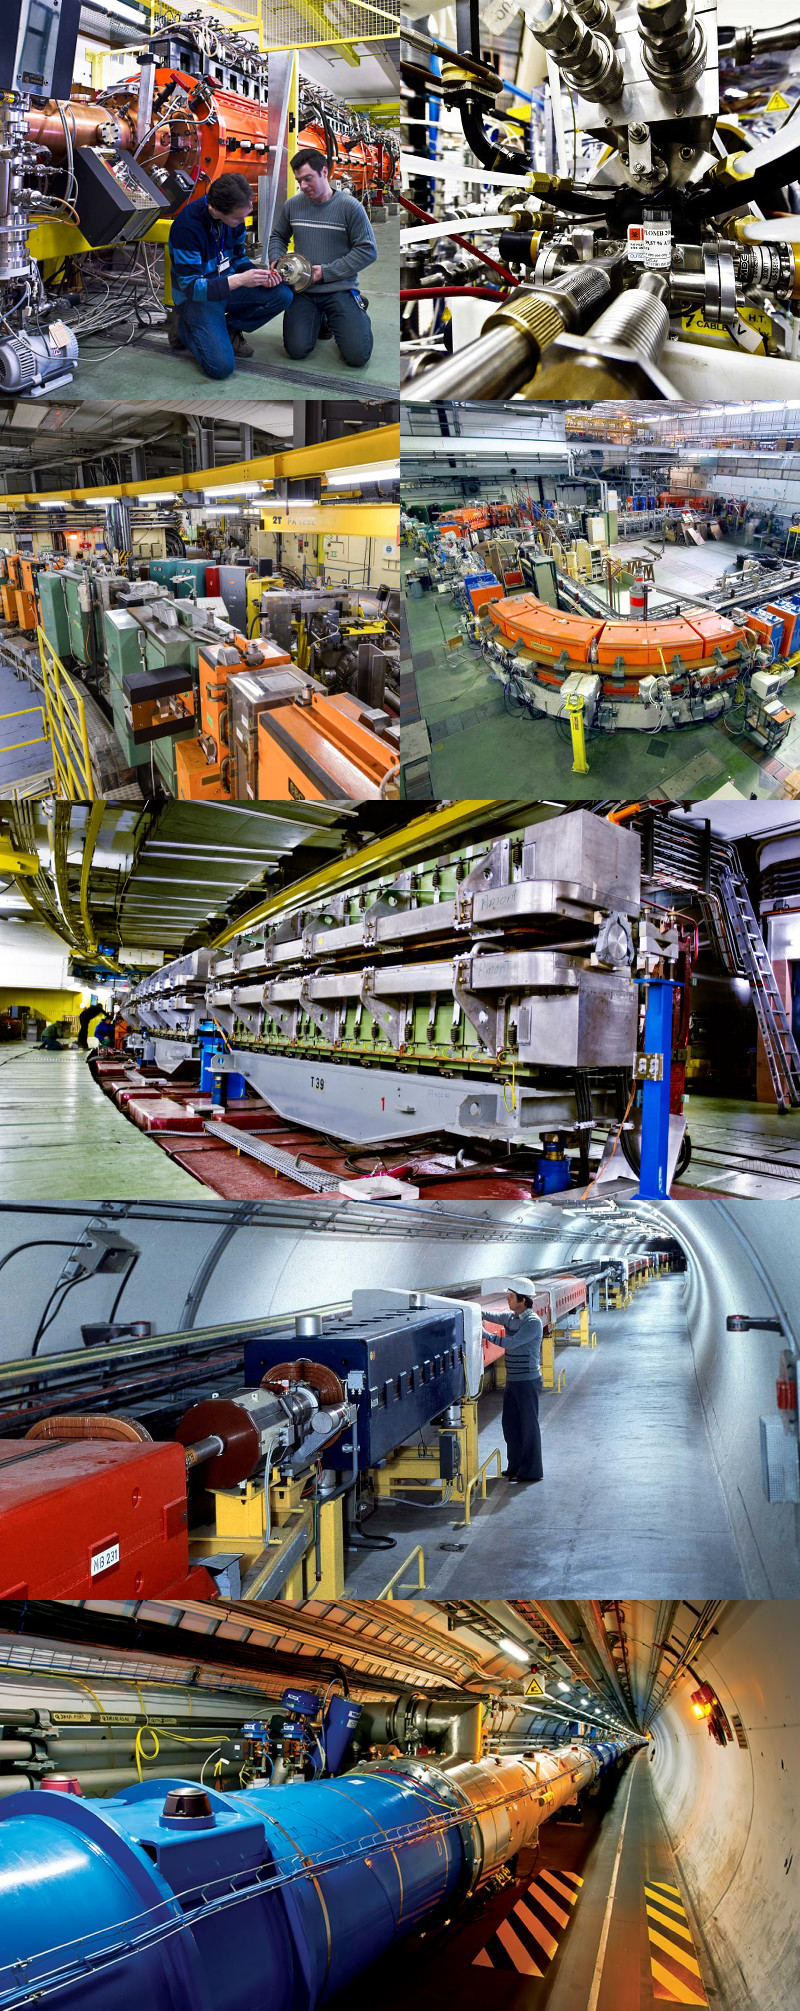
\includegraphics[width=\linewidth]{fig/chapt2/CERN-accelerators.jpg}
		\caption{\label{fig:CERNAccelerators} Pictures of the different accelerators. From top to bottom: first the LINAC 2 and the $Pb$ source of LINAC 3. Then the Booster and the LEIR. Finally, the PS, the SPS and the LHC.}
	\end{wrapfigure}
	
	The LHC has always been considered as an option for the future of CERN. At the moment of the construction of the LEP beneath the border between France and Switzerland, the tunnel was built in order to accommodate what would be a \acl{LHC} with a dipole field of \SI{10}{T} and a beam energy in between 8 and \SI{9}{TeV}~\cite{ANNUALREPORT1984}. In 1985, the creation of a 'Working Group on the Scientific and Technological Future of CERN' took place to investigate such a collider~\cite{ANNUALREPORT1985}. The decision was finally taken almost ten years later, in 1994, to construct the LHC in the LEP tunnel~\cite{ANNUALREPORT1994} and the approval of the 4 main experiments that would take place at the four interaction points came in 1997~\cite{ANNUALREPORT1997} and 1998~\cite{ANNUALREPORT1998}:
		
	\begin{itemize}
		\item[•] ALICE~\cite{ALICELOI} has been designed for the purpose of studying the confinement of quarks through exploration of the quark-gluon plasma that is believed to have been a state of matter that existed in the very first moment of the universe.
		\item[•] ATLAS~\cite{ATLASLOI} and CMS~\cite{CMSLOI} are general purpose experiments that have been designed with the goal of continuing the exploration of the Standard Model and the investigation of new physics.
		\item[•] LHCb~\cite{LHCBLOI} has been designed to investigate the preference of matter over antimatter in the universe through CP violation.
	\end{itemize}
	
	These large-scale experiments, as well as the full CERN accelerator complex, are displayed in Figure~\ref{fig:CERNComplex}. The LHC is a \SI{27}{km} long hadron collider and the most powerful accelerator used for particle physics since 2008~\cite{LHC2008}. The LHC is designed to collide protons at a center-of-mass energy of \SI{14}{TeV} and luminosity of \Ord{34} \si{cm^{-2}s^{-1}}, as well as $Pb$ ions at a center-of-mass energy of \SI{2.8}{TeV/A} with a peak luminosity of \Ord{27} \si{cm^{-2}s^{-1}}. The collider is the last of a long series of accelerating devices. Indeed, before being accelerated by the LHC, the particles need to pass through different acceleration stages. All these acceleration stages are visible on Figure~\ref{fig:CERNComplex} and pictures of the accelerators are shown in Figure~\ref{fig:CERNAccelerators}.
	
\endgroup
\begingroup\setlength{\intextsep}{5pt}\setlength{\columnsep}{15pt}
	
	\begin{wrapfigure}{l}{.45\linewidth}
		\begin{minipage}{\linewidth}
			\centering\captionsetup[subfigure]{justification=centering}
			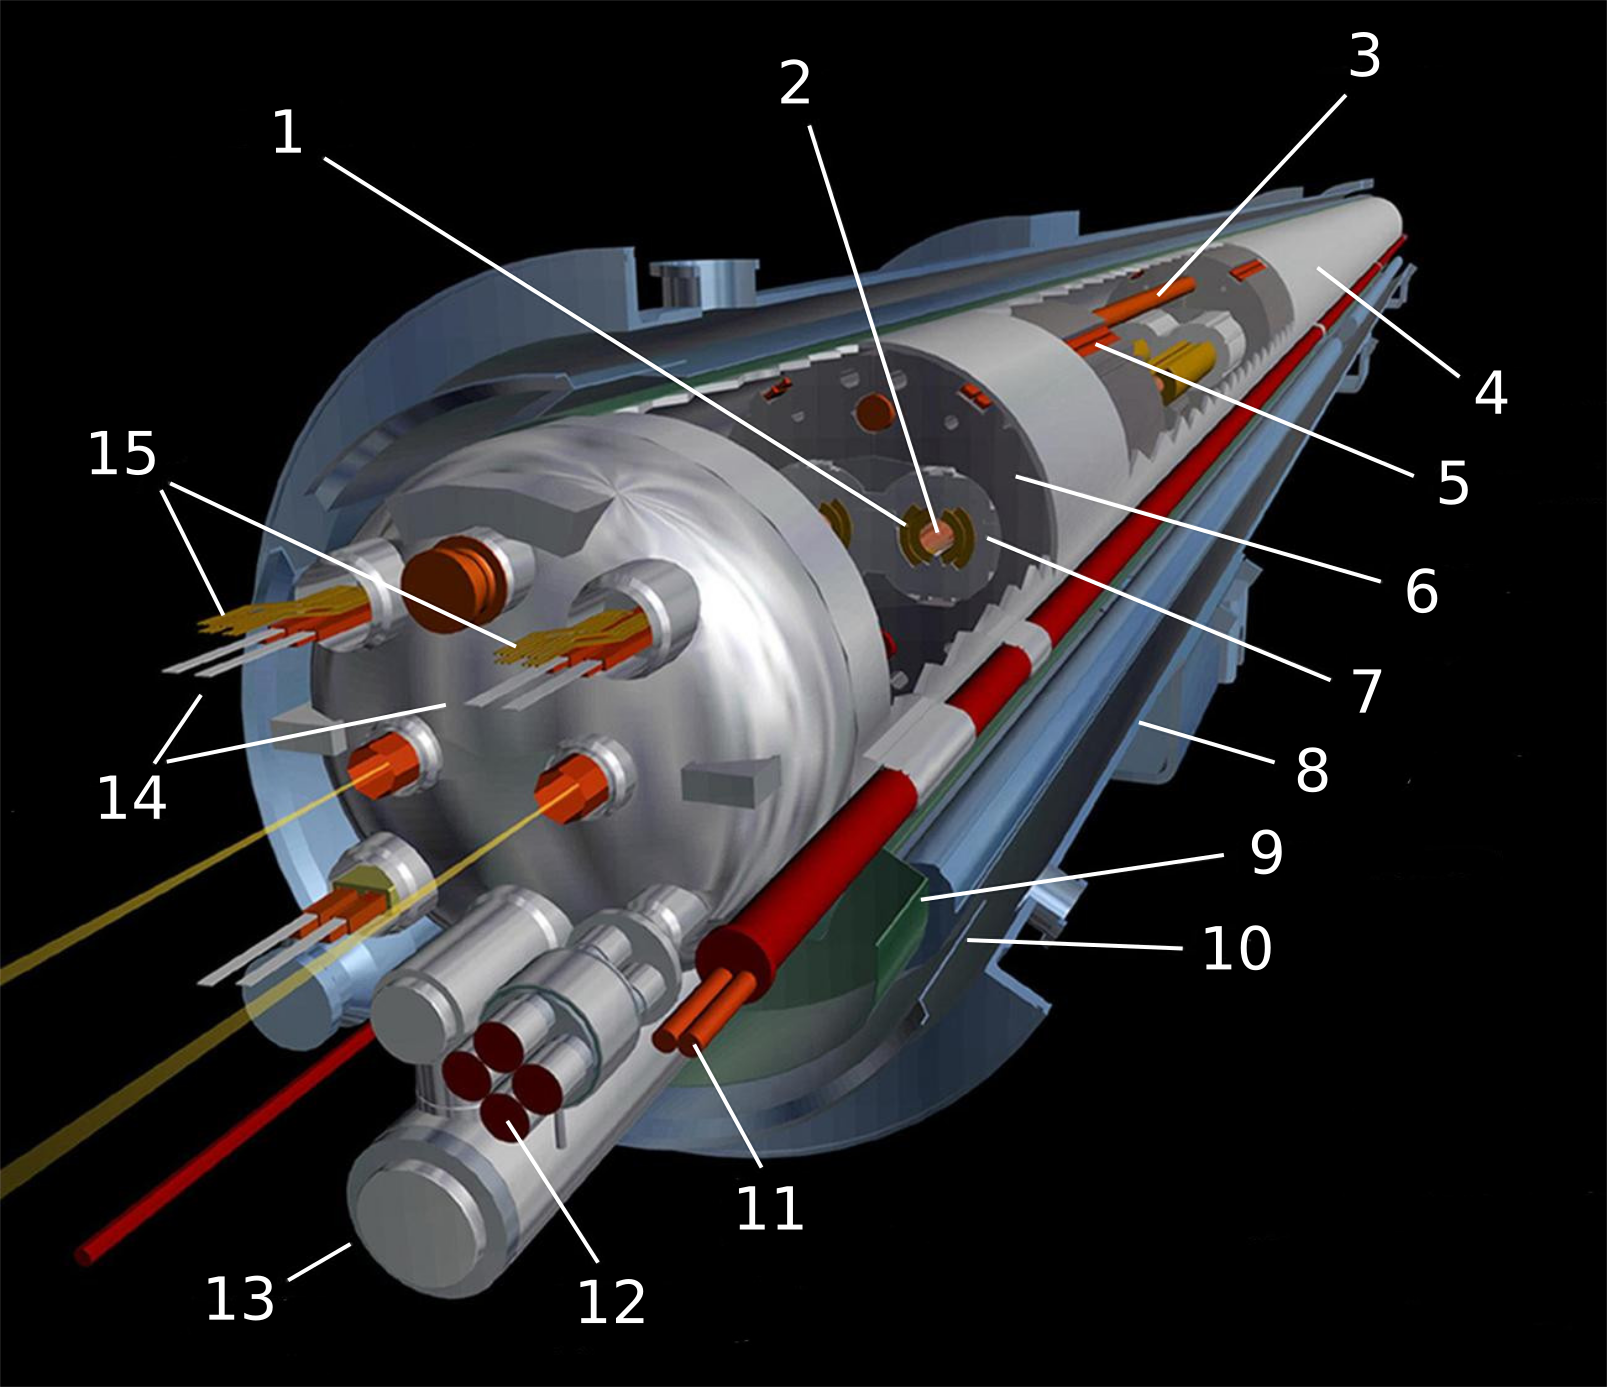
\includegraphics[width = \linewidth]{fig/chapt2/LHC-dipole.png}
			\subcaption{\label{fig:LHCDipole:A}}
			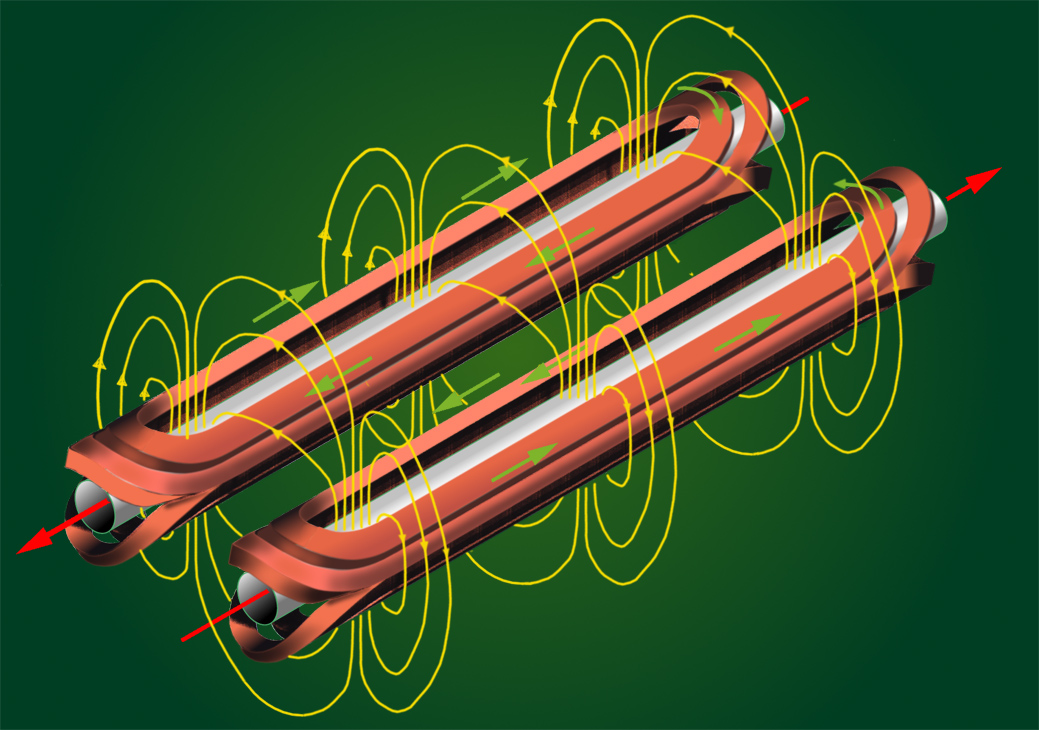
\includegraphics[width = \linewidth]{fig/chapt2/LHC-dipole-field.jpg}
			\subcaption{\label{fig:LHCDipole:B}}
		\end{minipage}
		\caption{\label{fig:LHCDipole} Figure~\ref{fig:LHCDipole:A}: schematics of the LHC cryodipoles. 1: Superconducting Coils, 2: Beam pipe, 3: Heat exchanger Pipe, 4: Helium-II Vessel, 5: Superconducting Bus-bar, 6: Iron Yoke, 7: Non-Magnetic Collars, 8: Vacuum Vessel, 9: Radiation Screen, 10: Thermal Shield, 11: Auxiliary Bus-bar Tube, 12: Instrumentation Feed Throughs, 13: Protection Diode, 14: Quadrupole Bus-bars, 15: Spool Piece Bus-bars. Figure~\ref{fig:LHCDipole:B}: magnetic field and resulting motion force applied on the beam particles.}
	\end{wrapfigure}
	
	The story of accelerated protons at CERN starts with a bottle of hydrogen gas injected into the source chamber of the linear particle accelerator \textit{LINAC 2} in which a strong electric field strips the electron off the hydrogen molecules only to keep their nuclei, the protons. The cylindrical conductors then accelerate the protons to an energy of \SI{50}{MeV}.
	When exiting the LINAC 2, the protons are divided into four bunches and injected into the four superimposed synchrotron rings of the \textit{Booster} where they are then accelerated to reach an energy of \SI{1.4}{GeV} before being injected into the \textit{PS}.
	The four proton bunches are hence sent as one to the PS where their energy eventually reaches \SI{26}{GeV}. The PS not only accelerates protons. It also accelerates heavy ions from the \textit{\acf{LEIR}}. Lead is first injected into the dedicated linear collider \textit{LINAC 3}, that accelerates the ions. Electrons are striped off the lead ions all along the acceleration process and eventually, only bare nuclei are injected in the LEIR whose goal is to transform the long ion pulses received into short dense bunches for LHC. Ions injected and stored in the PS were accelerated by the LEIR from \SI{4.2}{MeV} to \SI{72}{MeV}.
	Directly following the PS, is finally the last acceleration stage before the LHC, the \SI{7}{km} long \textit{SPS}. The SPS accelerates the protons to \SI{450}{GeV} and inject them in both LHC accelerator rings that will increase their energy up to \SI{7}{TeV}. When the LHC runs with heavy lead ions for ALICE and LHCb, ions are injected and accelerated to reach the energy of \SI{2.8}{TeV/A}.
	
	The LHC beams are not continuous but are rather organised in bunches of particles. When in $pp$-collision mode, the beams are composed of 2808 bunches of \Sci{1.15}{11} protons separated by \SI{25}{ns}. When in $Pb$-collision mode, the 592 $Pb$ bunches are on the contrary composed of \Sci{2.2}{8} ions separated by \SI{100}{ns}. The two parallel proton beams of the LHC are contained in a single twin-bore magnet due to the space restriction in the LEP tunnel. Indeed, building two completely separate accelerator rings next to each other was impossible. The dipoles of the 1232 twin-bore magnets are shown in Figure~\ref{fig:LHCDipole} alongside the magnetic field generated along the dipole section to accelerate the particles. The dipoles generate a nominal field of \SI{8.33}{T}, needed to give protons and lead nucleons their nominal energy. Some 392 quadrupoles, presented in Figure~\ref{fig:LHCQuadrupole}, are also used to focus to the beams, as well as other multipoles to correct smaller imperfections.
	
\endgroup
	
	\begin{figure}[H]
		\begin{subfigure}{0.5\linewidth}
			\centering
			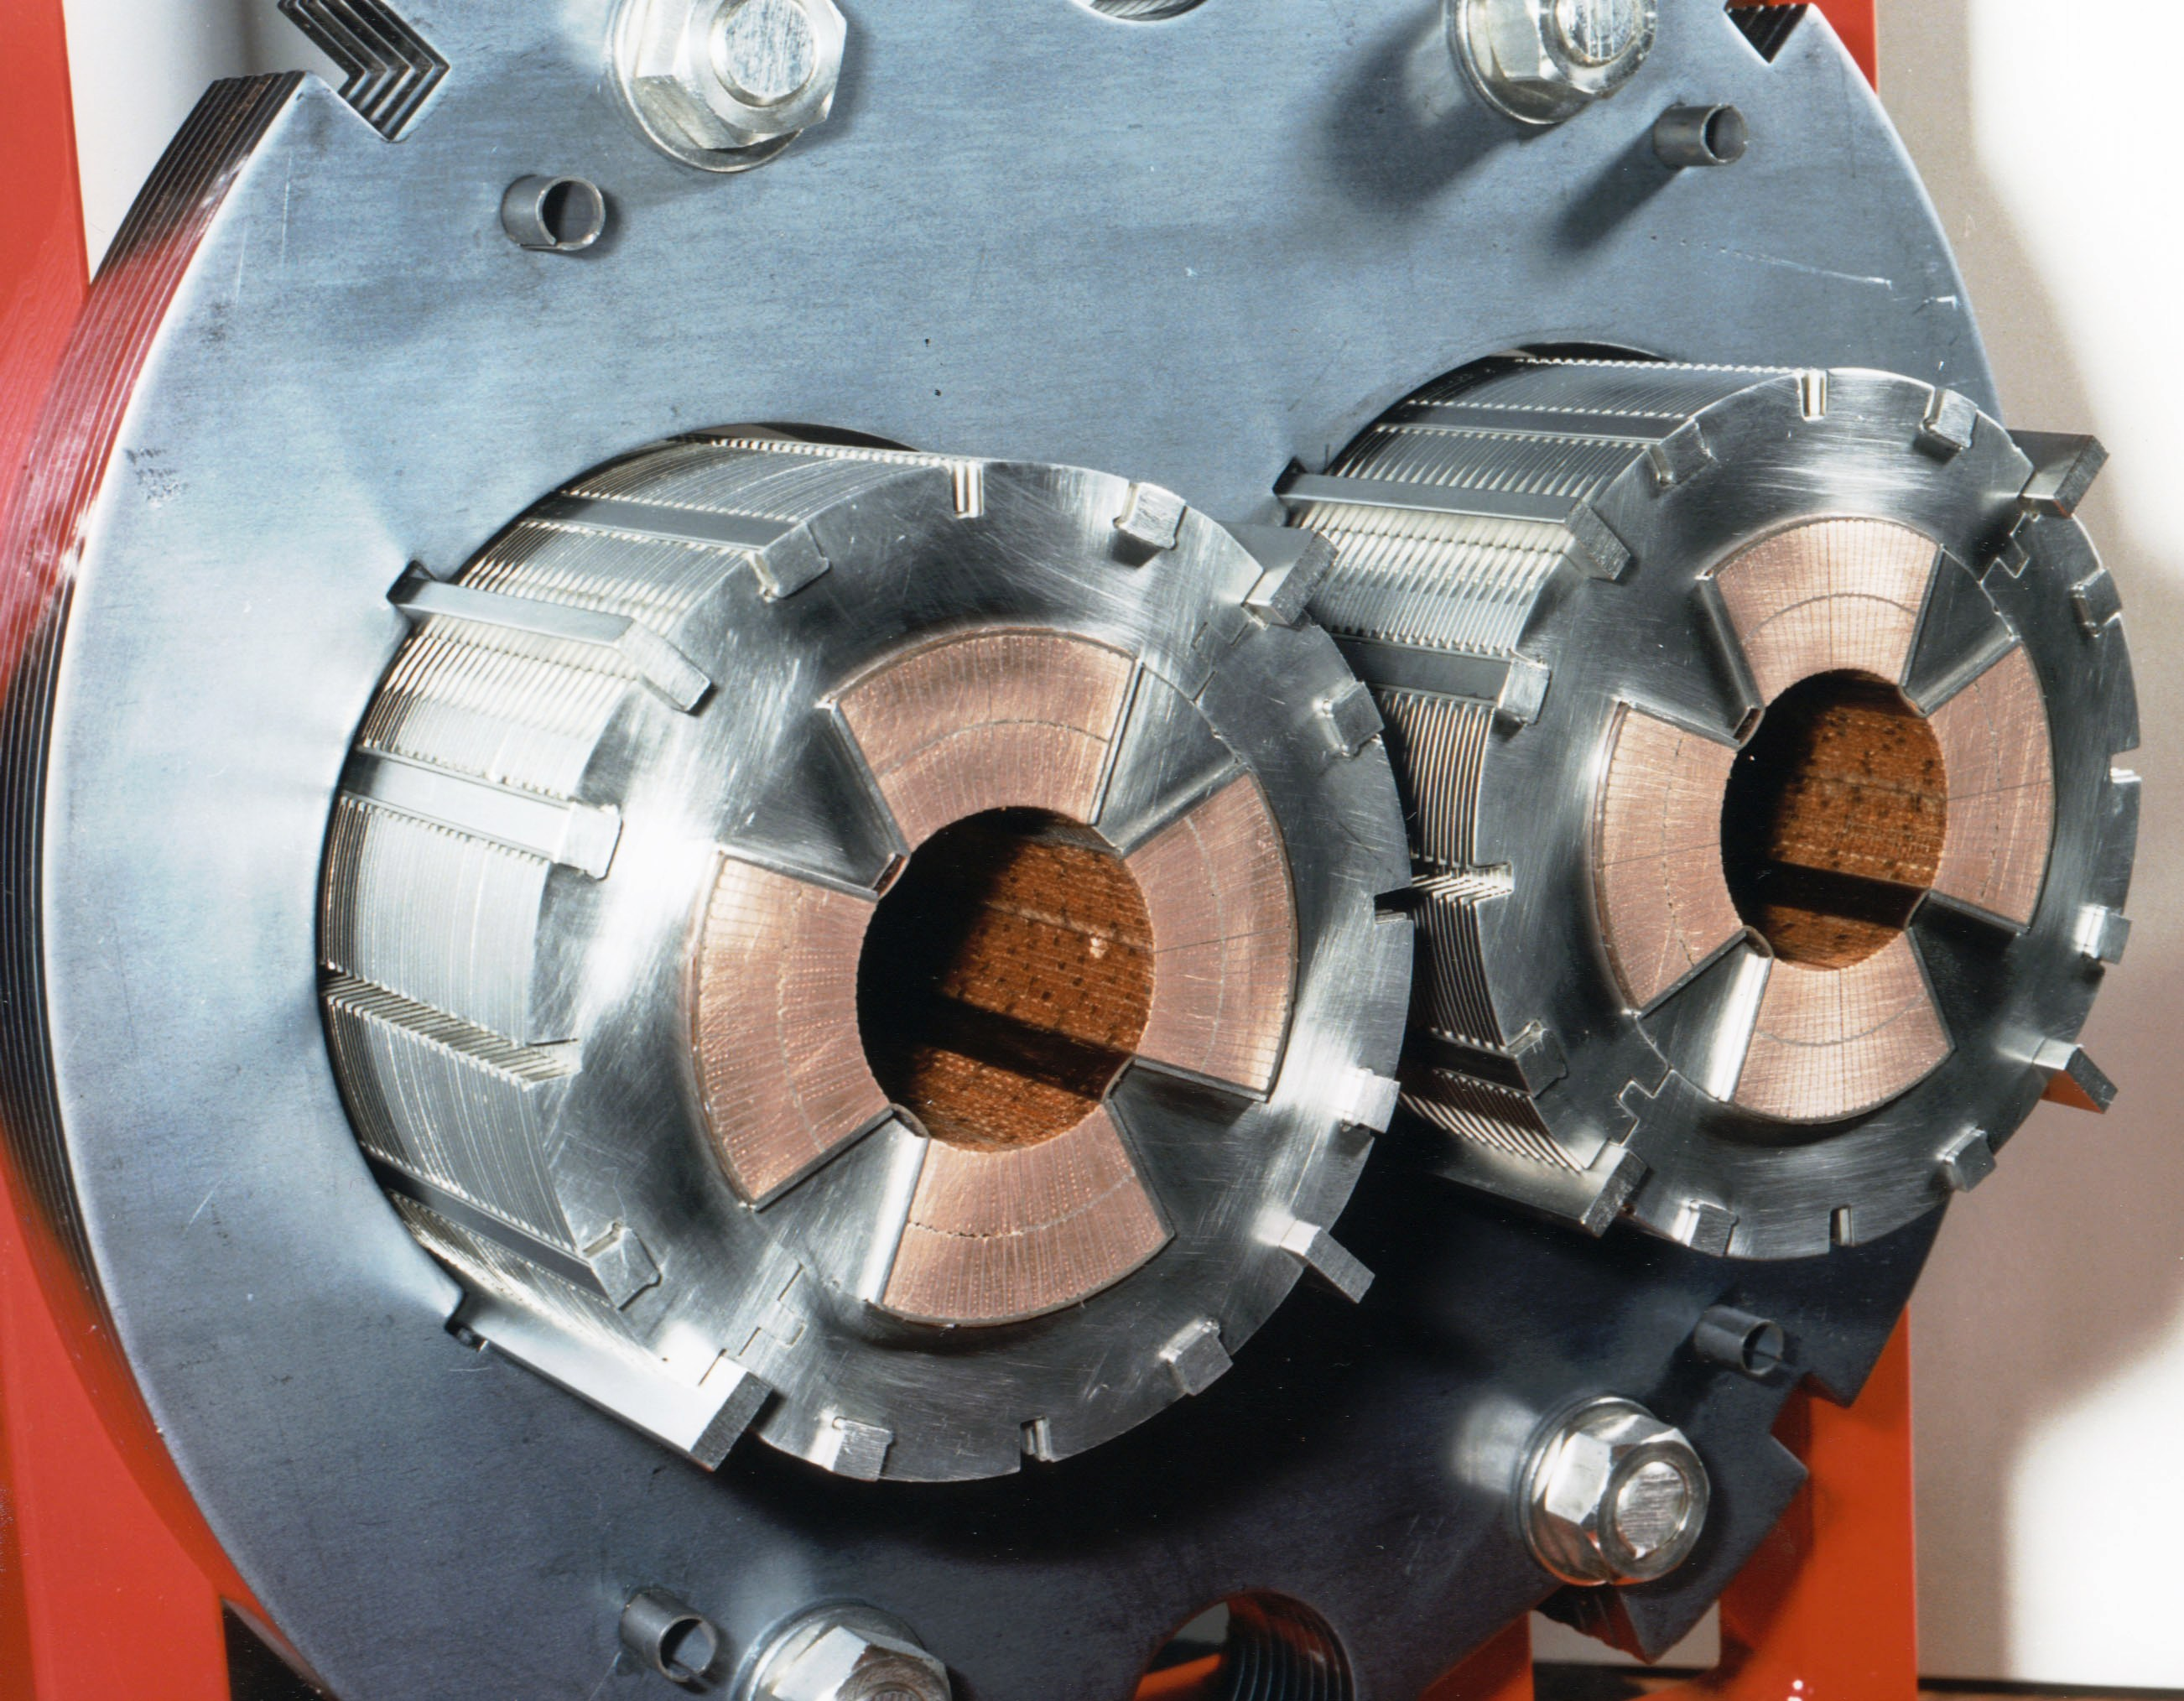
\includegraphics[height = 4cm]{fig/chapt2/LHC-quadrupole.jpg}
			\caption{\label{fig:LHCQuadrupole:A}}
		\end{subfigure}
		\begin{subfigure}{0.5\linewidth}
			\centering
			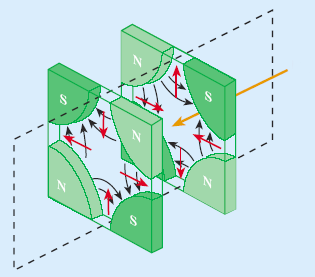
\includegraphics[height = 4cm]{fig/chapt2/LHC-quadrupole-field.png}
			\caption{\label{fig:LHCQuadrupole:B}}
		\end{subfigure}
		\caption{\label{fig:LHCQuadrupole} The LHC quadrupoles (Figure~\ref{fig:LHCQuadrupole:A}) showed together with the magnetic fields and resulting focussing force applied on the beam by two consecutive quadrupoles (Figure~\ref{fig:LHCQuadrupole:B}).}
	\end{figure}
	
	\subsection{Timeline of operation}
	\label{chapt2:ssec:timeline}
	
	LHC accelerated its first proton in September 2008 but the first collisions only started one year later in November 2009. At this moment the LHC machine officially became the world's most powerful particle accelerator and entered its Physics Run 1 that lasted until February 2013. During Run 1 of the LHC program, the center-of-mass energy was only half of the nominal LHC energy. Nevertheless, the energy and luminosity displayed during Run 1 were enough for both CMS and ATLAS to discover the Higgs boson~\cite{ATLAS2012,CMS2012} as showed in Figure~\ref{fig:Higgs} and for LHCb to discover pentaquarks~\cite{PENTAQUARK2015} and confirm the existence of tetraquarks~\cite{TETRAQUARK2017}. During this period, ALICE also reported a successful observation of the quark-gluon plasma aimed at studying the early universe~\cite{ALICEINFO}, ATLAS reported the observation of a new particle before the discovery of the Higgs~\cite{CHIB2012} and a first test of super-symmetric models was performed~\cite{B0SDECAY2013}.
	
	\begin{figure}[H]
		\begin{subfigure}{0.5\linewidth}
			\centering
			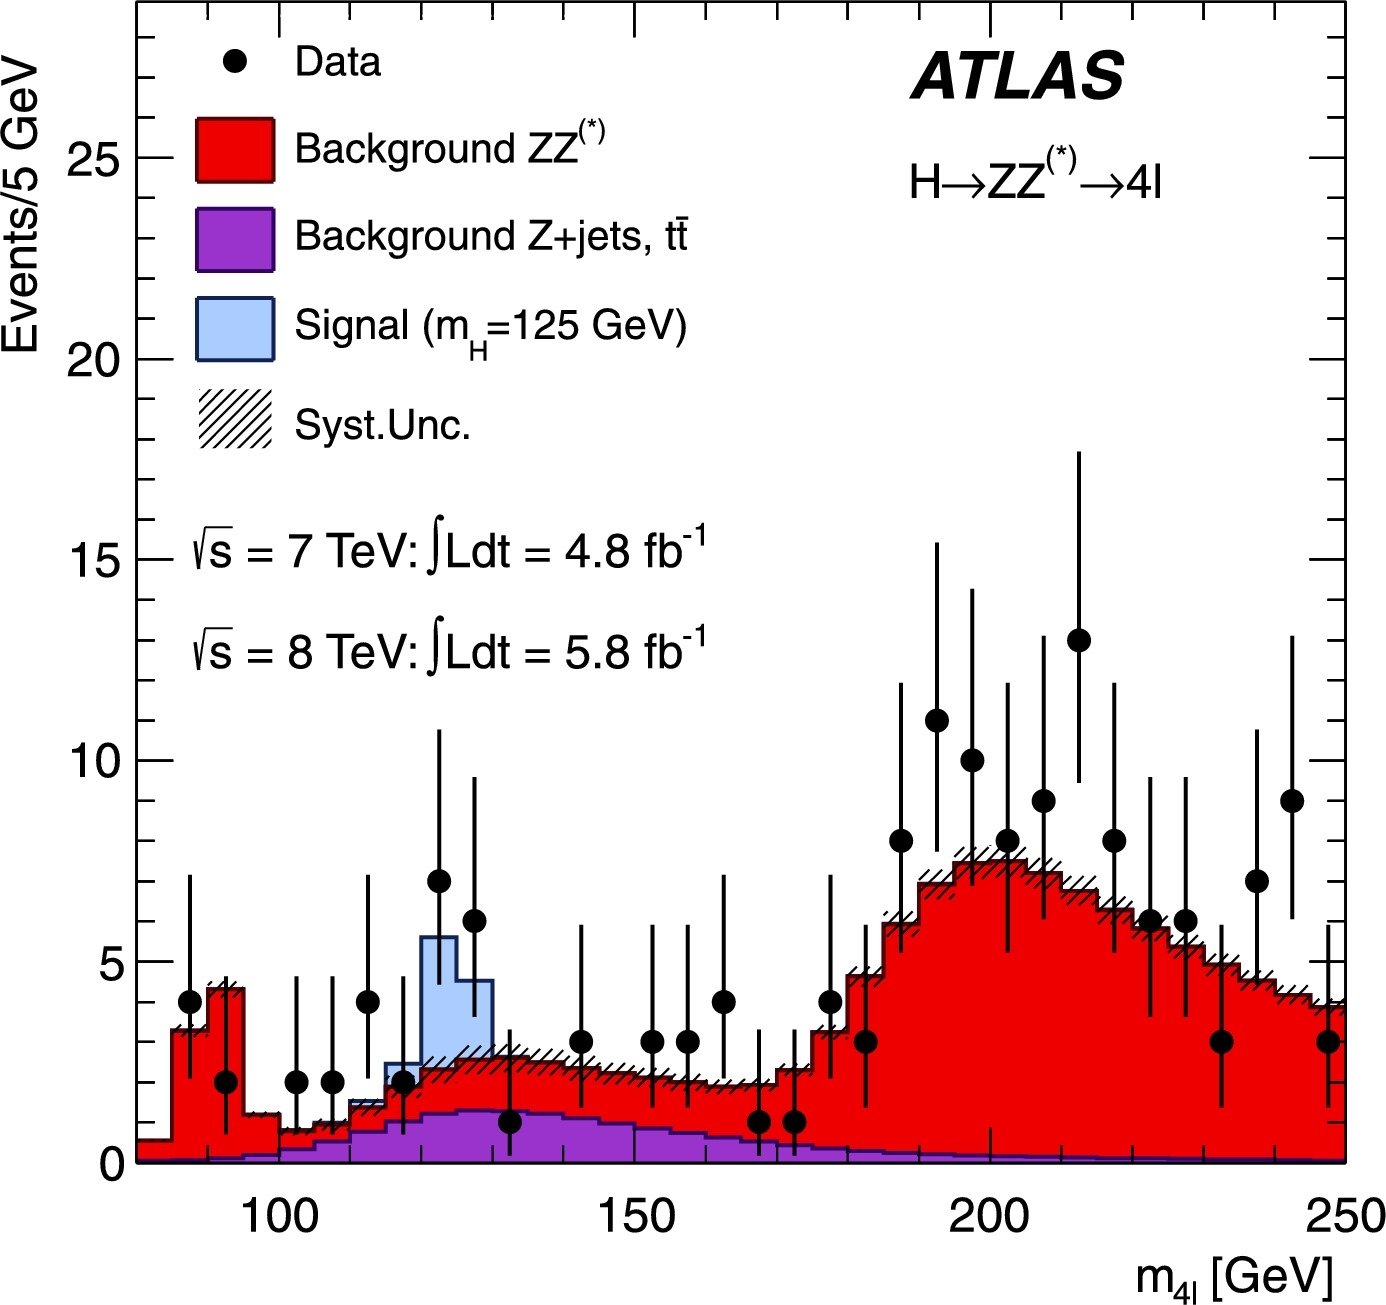
\includegraphics[height = 6cm]{fig/chapt2/Higgs-ATLAS-ZZ-4l.jpg}
			\caption{\label{fig:Higgs:A}}
		\end{subfigure}
		\begin{subfigure}{0.5\linewidth}
			\centering
			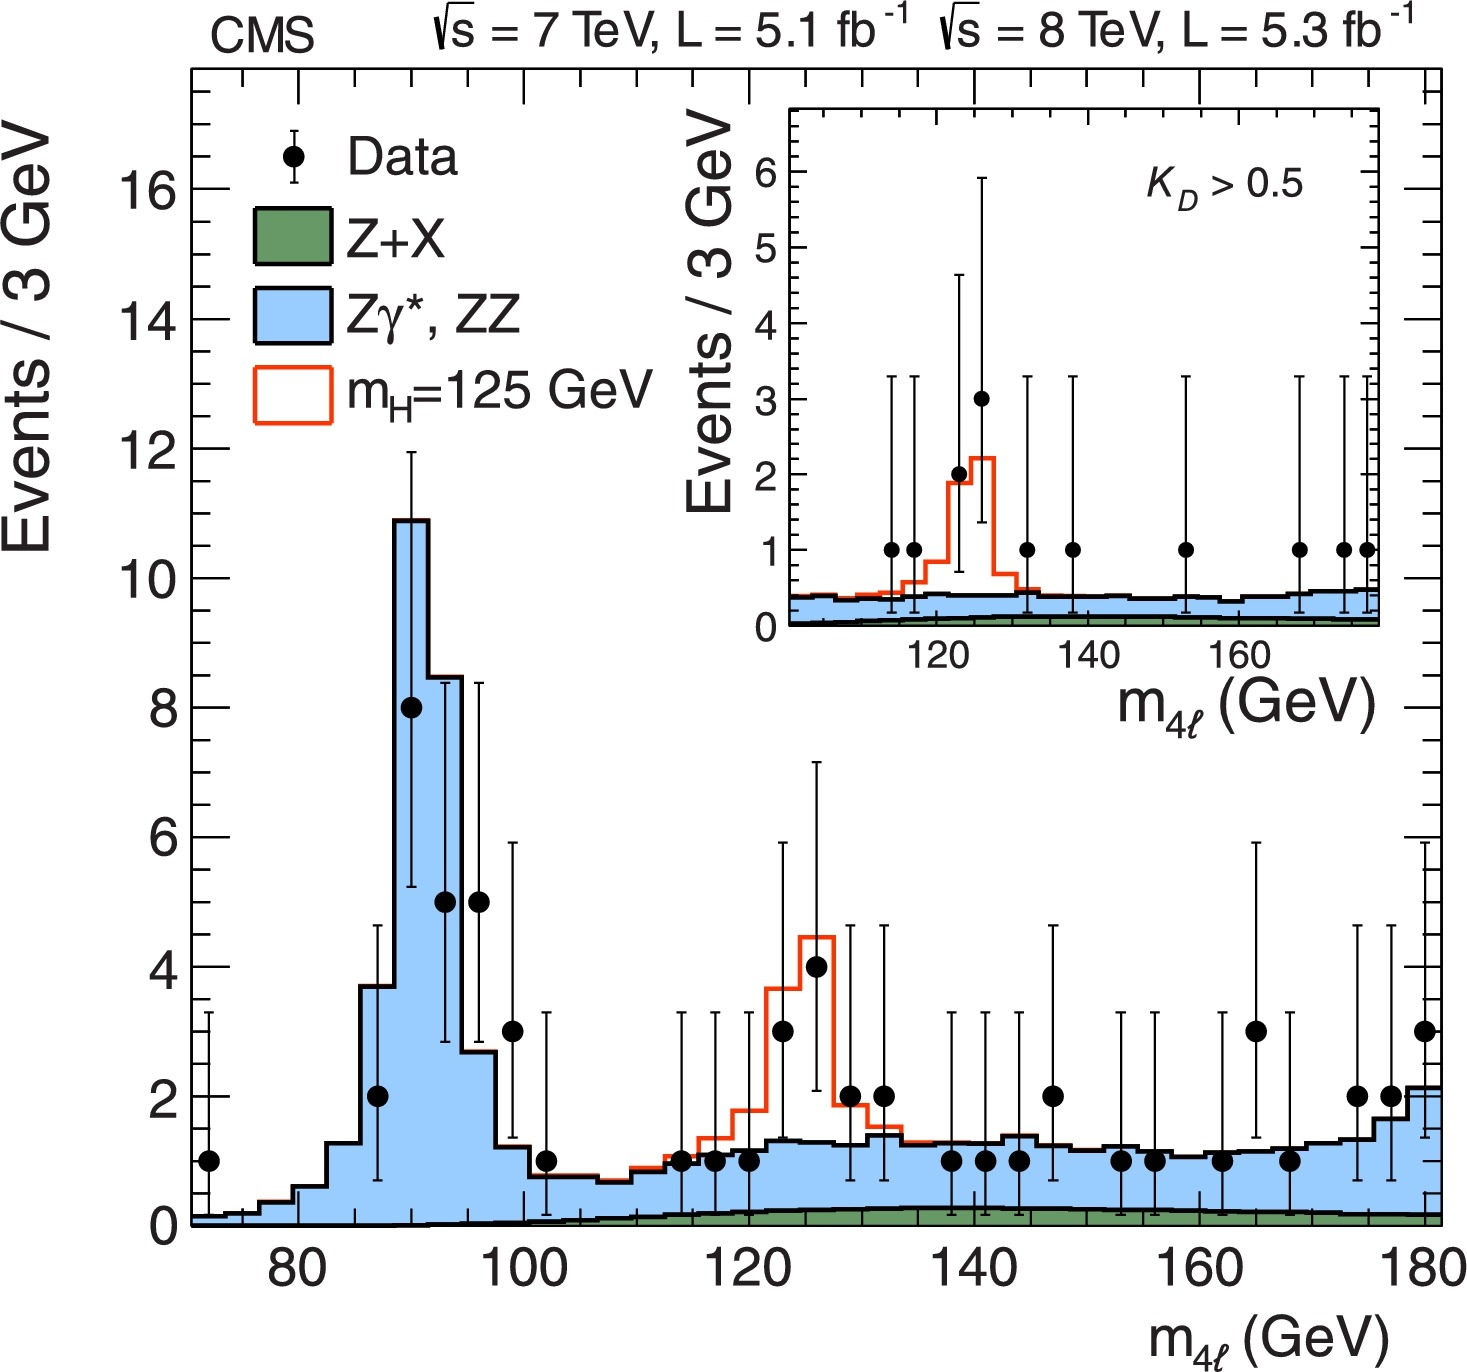
\includegraphics[height = 6cm]{fig/chapt2/Higgs-CMS-ZZ-4l.jpg}
			\caption{\label{fig:Higgs:B}}
		\end{subfigure}
		\caption{\label{fig:Higgs} Distribution of the four-lepton invariant mass for the $ZZ \rightarrow 4l$ analysis as presented by both ATLAS~\cite{ATLAS2012} and CMS~\cite{CMS2012} in 2012.}
	\end{figure}
	
	Run 1 was brought to an end with the start of the \acl{LS1}, an almost two years technical stop aimed at increasing the energy of the center-of-mass collisions to $\sqrt{s} =$ \SI{13}{TeV} as well as the instantaneous luminosity. This maintenance stop was also effectively used by the experiments which upgraded part of their detection systems. Run 2 then started in 2015 and lasted until end of 2018 where the activities ended with a last heavy ion run. During the operation, the instantaneous was successfully brought to a value of \Sci{1.7}{34}\siflux exceeding the design value. Run 2 has been the occasion to acquire more data to study the properties of the Higgs boson with more precision. The boson discovered in the first physics run seems to be consistent with the SM Higgs boson~\cite{HIGGS2015}.
	
	\begin{figure}[H]
		\begin{subfigure}{\linewidth}
			\centering
			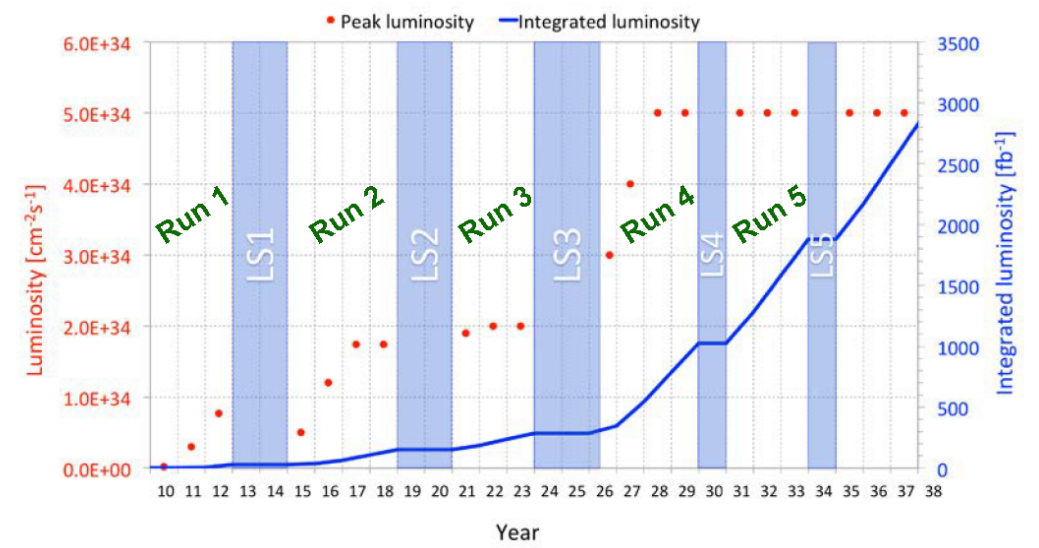
\includegraphics[width=\plotwidth]{fig/chapt2/HL-LHC-nominal.png}
			\caption{\label{fig:HL-LHC-Timeline:A}}
		\end{subfigure}
		\begin{subfigure}{\linewidth}
			\centering
			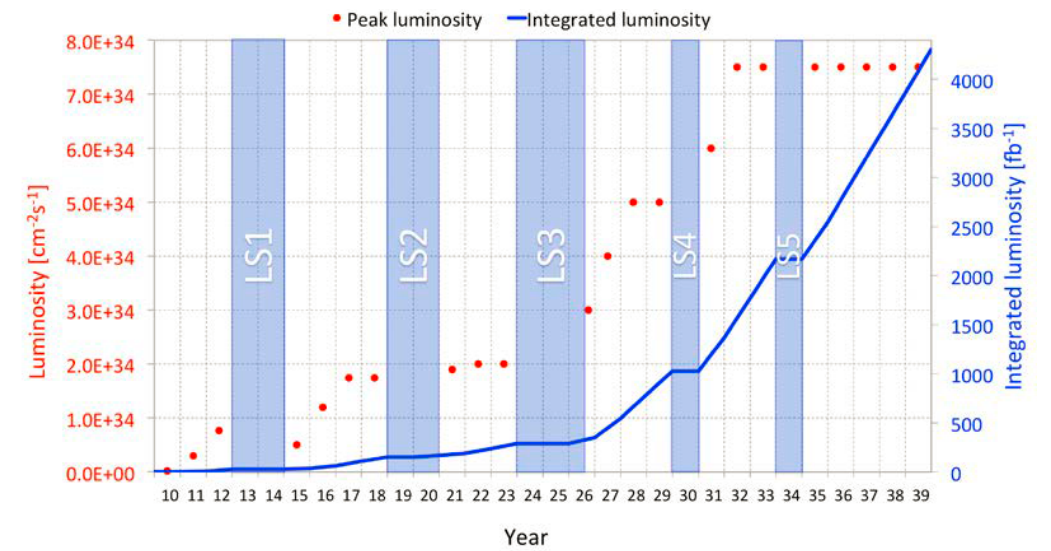
\includegraphics[width=\plotwidth]{fig/chapt2/HL-LHC-ultimate.png}
			\caption{\label{fig:HL-LHC-Timeline:B}}
		\end{subfigure}
		\caption{\label{fig:HL-LHC-Timeline} Detailed timeline projection of LHC and HL-LHC operation until 2039 showing the evolution of the instantaneous and integrated luminosity as designed (Figure~\ref{fig:HL-LHC-Timeline:A}) and in the ultimate case where the instantaneous luminosity is increased to \Sci{7.5}{34}\siflux thanks to a new increase of instantaneous luminosity during Run 5 (Figure~\ref{fig:HL-LHC-Timeline:B})~\cite{HLLHC2017,HLLHCPDR,PHASEIITP}.}
	\end{figure}
	
	From the end of 2018 to early 2021 the \acl{LS2} will take place. This second maintenance stop will be the occasion to boost once again the beam energy to finally reach the design energy of LHC, \SI{14}{TeV}. On the side of the maintenance work, preliminary work for the \acl{HL-LHC} will be performed. The preparations will consist of detector, on the side of the experiments, and beam machine upgrades, on the side of LHC. In 2021, the physics program will be resumed with an instantaneous liminosity fixed at \Sci{2}{34}\siflux. During these 3 years of run, the LHC will deliver as much integrated luminosity as what what brought during the almost 7 years of both Run 1 and 2 of data taking. Phase-1 will end with an overall \SI{300}{fb^{-1}} delivered. The timeline so far described is summarized through the evolution of the instantaneous luminosity and of the corresponding integrated luminosity provided in Figure~\ref{fig:HL-LHC-Timeline}.
	
	After the \acl{LS3} (2024-2026) that will close the activities of Run 3, the accelerator will enter the HL-LHC configuration~\cite{HLLHC2017}, increasing the instantaneous luminosity to an unprecedented level of \Sci{5}{34}\siflux for $pp$-collisions (\Sci{4.5}{27}\siflux for $Pb$-collisions), boosting the discovery potential of the LHC. The HL-LHC phase should last at least another 10 years depending on the breakthrough this machine would lead to. Already a new accelerating device, the FCC, as been proposed and is being investigated to prepare the future of high-energy physics after the LHC.
	
	\subsection{\acl{HL-LHC}}
	\label{chapt2:ssec:HL-LHC}
		
	After approximately fifteen years of operation, the LHC will undergo a new series of upgrades during the LS3 in order to boost its discovery potential as previously discussed. The period after LS3 is what is referred to HL-LHC or Phase-2. The goal is to aim for a luminosity 5 to 7 times stronger than the nominal one trying to reach even 10 times this value if possible~\cite{HLLHC2017,HLLHCPDR}. Increasing the luminosity means that the beam size at the collision points needs to be reduced to boost the number of collisions per bunch crossing. For this purpose, new focusing and bending magnets and collimators will be installed at the collision points as well as newly developed \textit{"crab cavities"} that will tilt the particle bunches just prior to the collisions by giving them transverse momentum and thus increasing their meeting area. In addition, the full proton injection line will be upgraded.
	
	On the experiments side, the \acf{PU} will be increased up to 150 to 200 interactions per bunch crossing in ATLAS and CMS, making necessary a strong upgrade of the trigger system and of the inner trackers and of the calorimeters. Both ATLAS and CMS will also need to upgrade the muon trigger at the level of their endcaps mainly focusing on the coverage near the beam line in order to increase the detection acceptance and event selection. Moreover, the increased luminosity will also lead to an increased background rate and a faster ageing of the detectors.

	The end of 2018 marked the beginning of LS2 and the start of Phase-2 upgrade activities. From the HL-LHC period onwards, i.e. past LS3, the performance degradation due to integrated radiation as well as the average number of inelastic collisions per bunch crossing will rise substantially. This has become a major challenge for all of the LHC experiments, like CMS, that were forced to address an upgrade program for Phase-2~\cite{PHASEIITP}. Dealing with the data from the muon detectors will force to upgrade the detectors and electronics towards the most recent technologies.

	\subsection{The \acl{CMS} experiment}
	\label{chapt2:ssec:CMS}
	
	Among the four main LHC experiments is the Compact Muon Solenoid used as a multipurpose tool to investigate the SM and the physics beyond its scope. The CMS apparatus in itself is the heaviest detector ever built starring a \SI{15}{m} diameter and a \SI{29}{m} length for a total weight of \SI{14}{kT}. A thick \SI{4}{T} solenoid magnet located at the beam interaction point hosts trackers and calorimeters. Extending in all directions around the magnet, heavy iron return yokes are installed to extend the magnetic field and support a muon system. The apparatus consists of a barrel, referring to the magnet and the detectors contained in it and the part of the muon system built directly in the cylinder around the magnet, and of two endcaps in the forward and backward region of the detector that closes the apparatus and complete the detection coverage along the beam line. A front view on the barrel is provided in Figure~\ref{fig:CMS} while a detailed view of the apparatus is given in Figure~\ref{fig:CMS-detail}.
	
\begingroup\setlength{\intextsep}{5pt}\setlength{\columnsep}{15pt}
	
	\begin{wrapfigure}{r}{.5\linewidth}
		\centering
		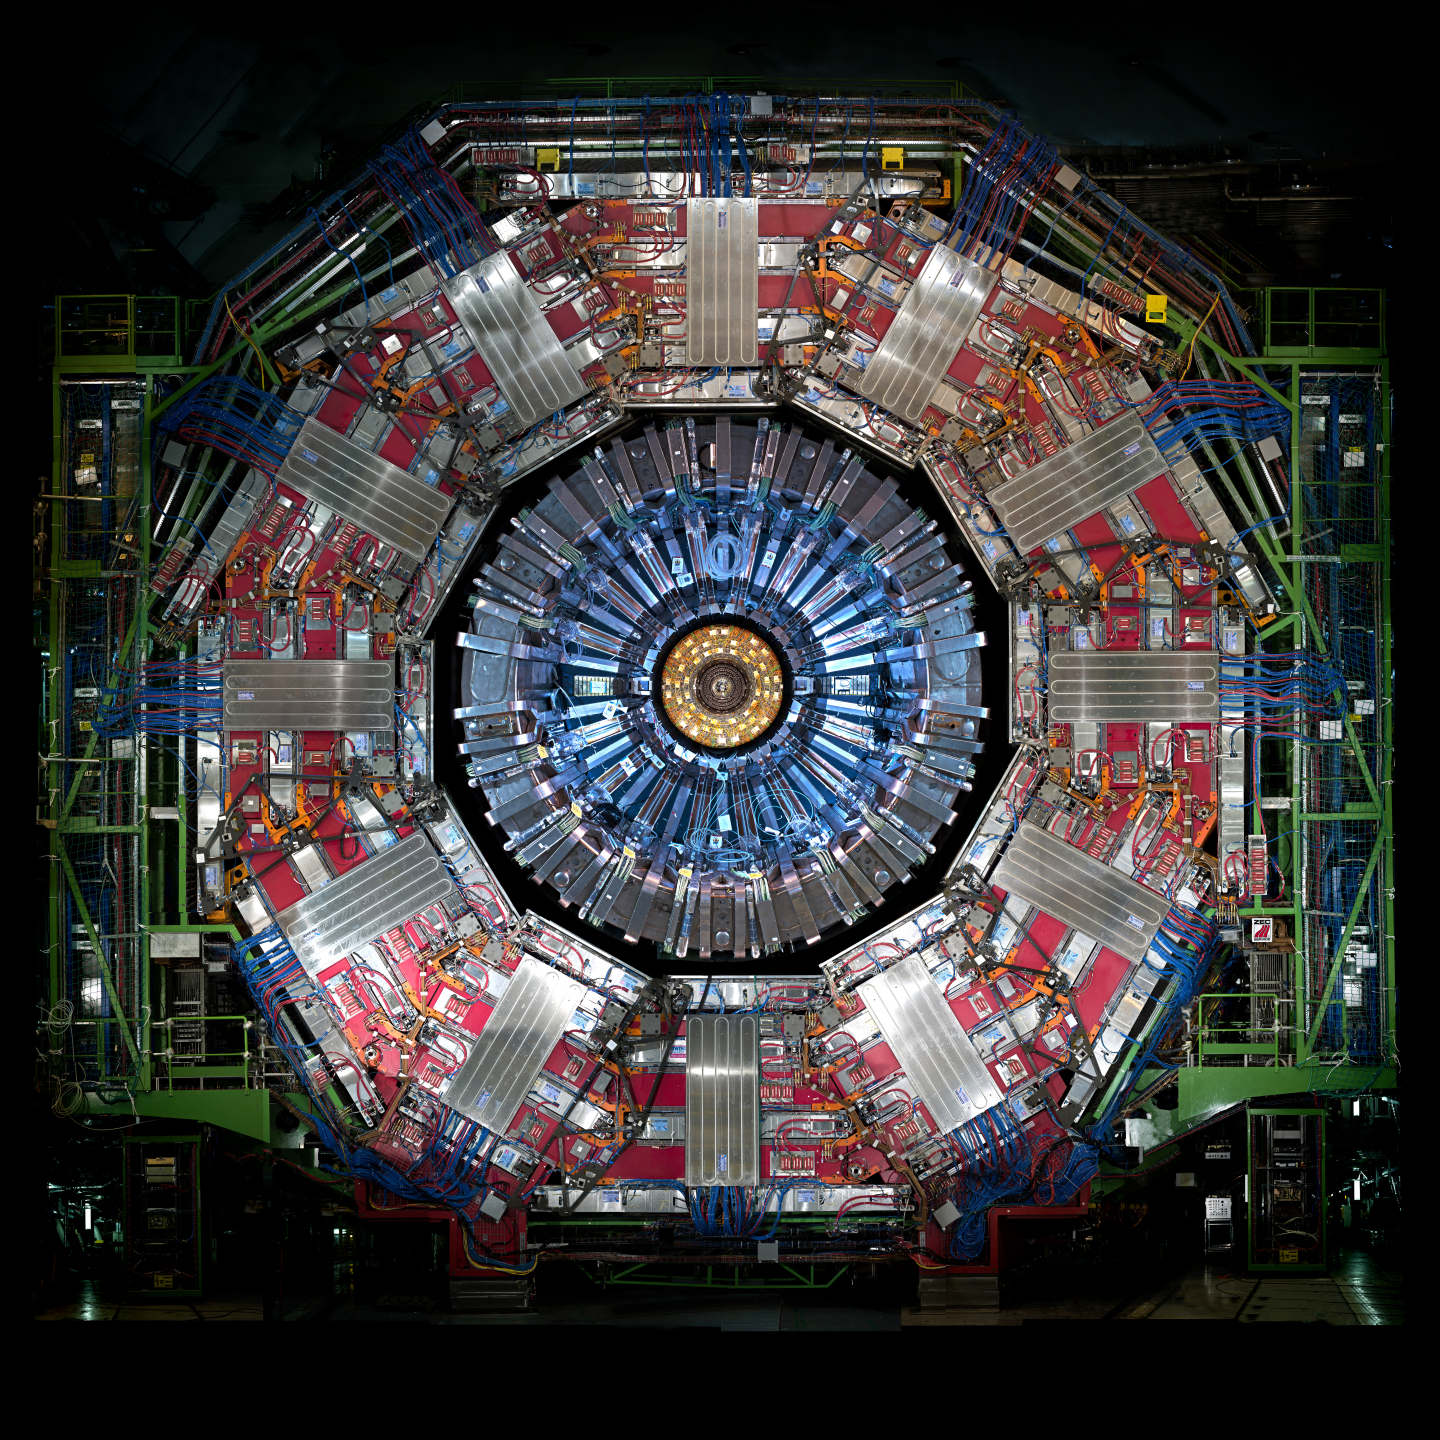
\includegraphics[width=\linewidth]{fig/chapt2/CMS.jpg}
		\caption{\label{fig:CMS} Picture of the CMS barrel. The red outer layer is the muon system hosted into the red iron return yokes. The calorimeters are the blue cylinder inside in magnet solenoid and the tracker is the inner yellow cylinder built around the beam pipe.}
	\end{wrapfigure}
	
	In order to efficiently detect all long living particles and measure their properties with good precision, the CMS detector uses an onion like layout around of the interaction point in order to maximize the covered solid angle. As detailed in Figure~\ref{fig:CMS-slice}, in the innermost region of the detector, closest to the interaction point, the silicon tracker records the trajectory of charged particles. Around it, the \acf{ECAL} stops and measures the energy deposition of electrons and photons. In the next layer, the \acf{HCAL}, hadrons are stopped are their energy measured. These layers are contained inside of the magnet of CMS, the superconducting solenoid. Outside of the magnet are the muon chambers embedded into iron return yokes used to control the magnetic field and gives muons, the only particles traveling completely through the whole detector, a double bending helping in reconstructing their energy and trajectory. Note that photons and neutral hadrons are differentiated from electrons and charged hadrons in the calorimeters by the fact that they don't interact with the silicon tracker and are not influenced by the magnetic field, as can be seen ni Figure~\ref{fig:CMS-slice}.
	
\endgroup
	
	\begin{figure}[H]
		\centering
		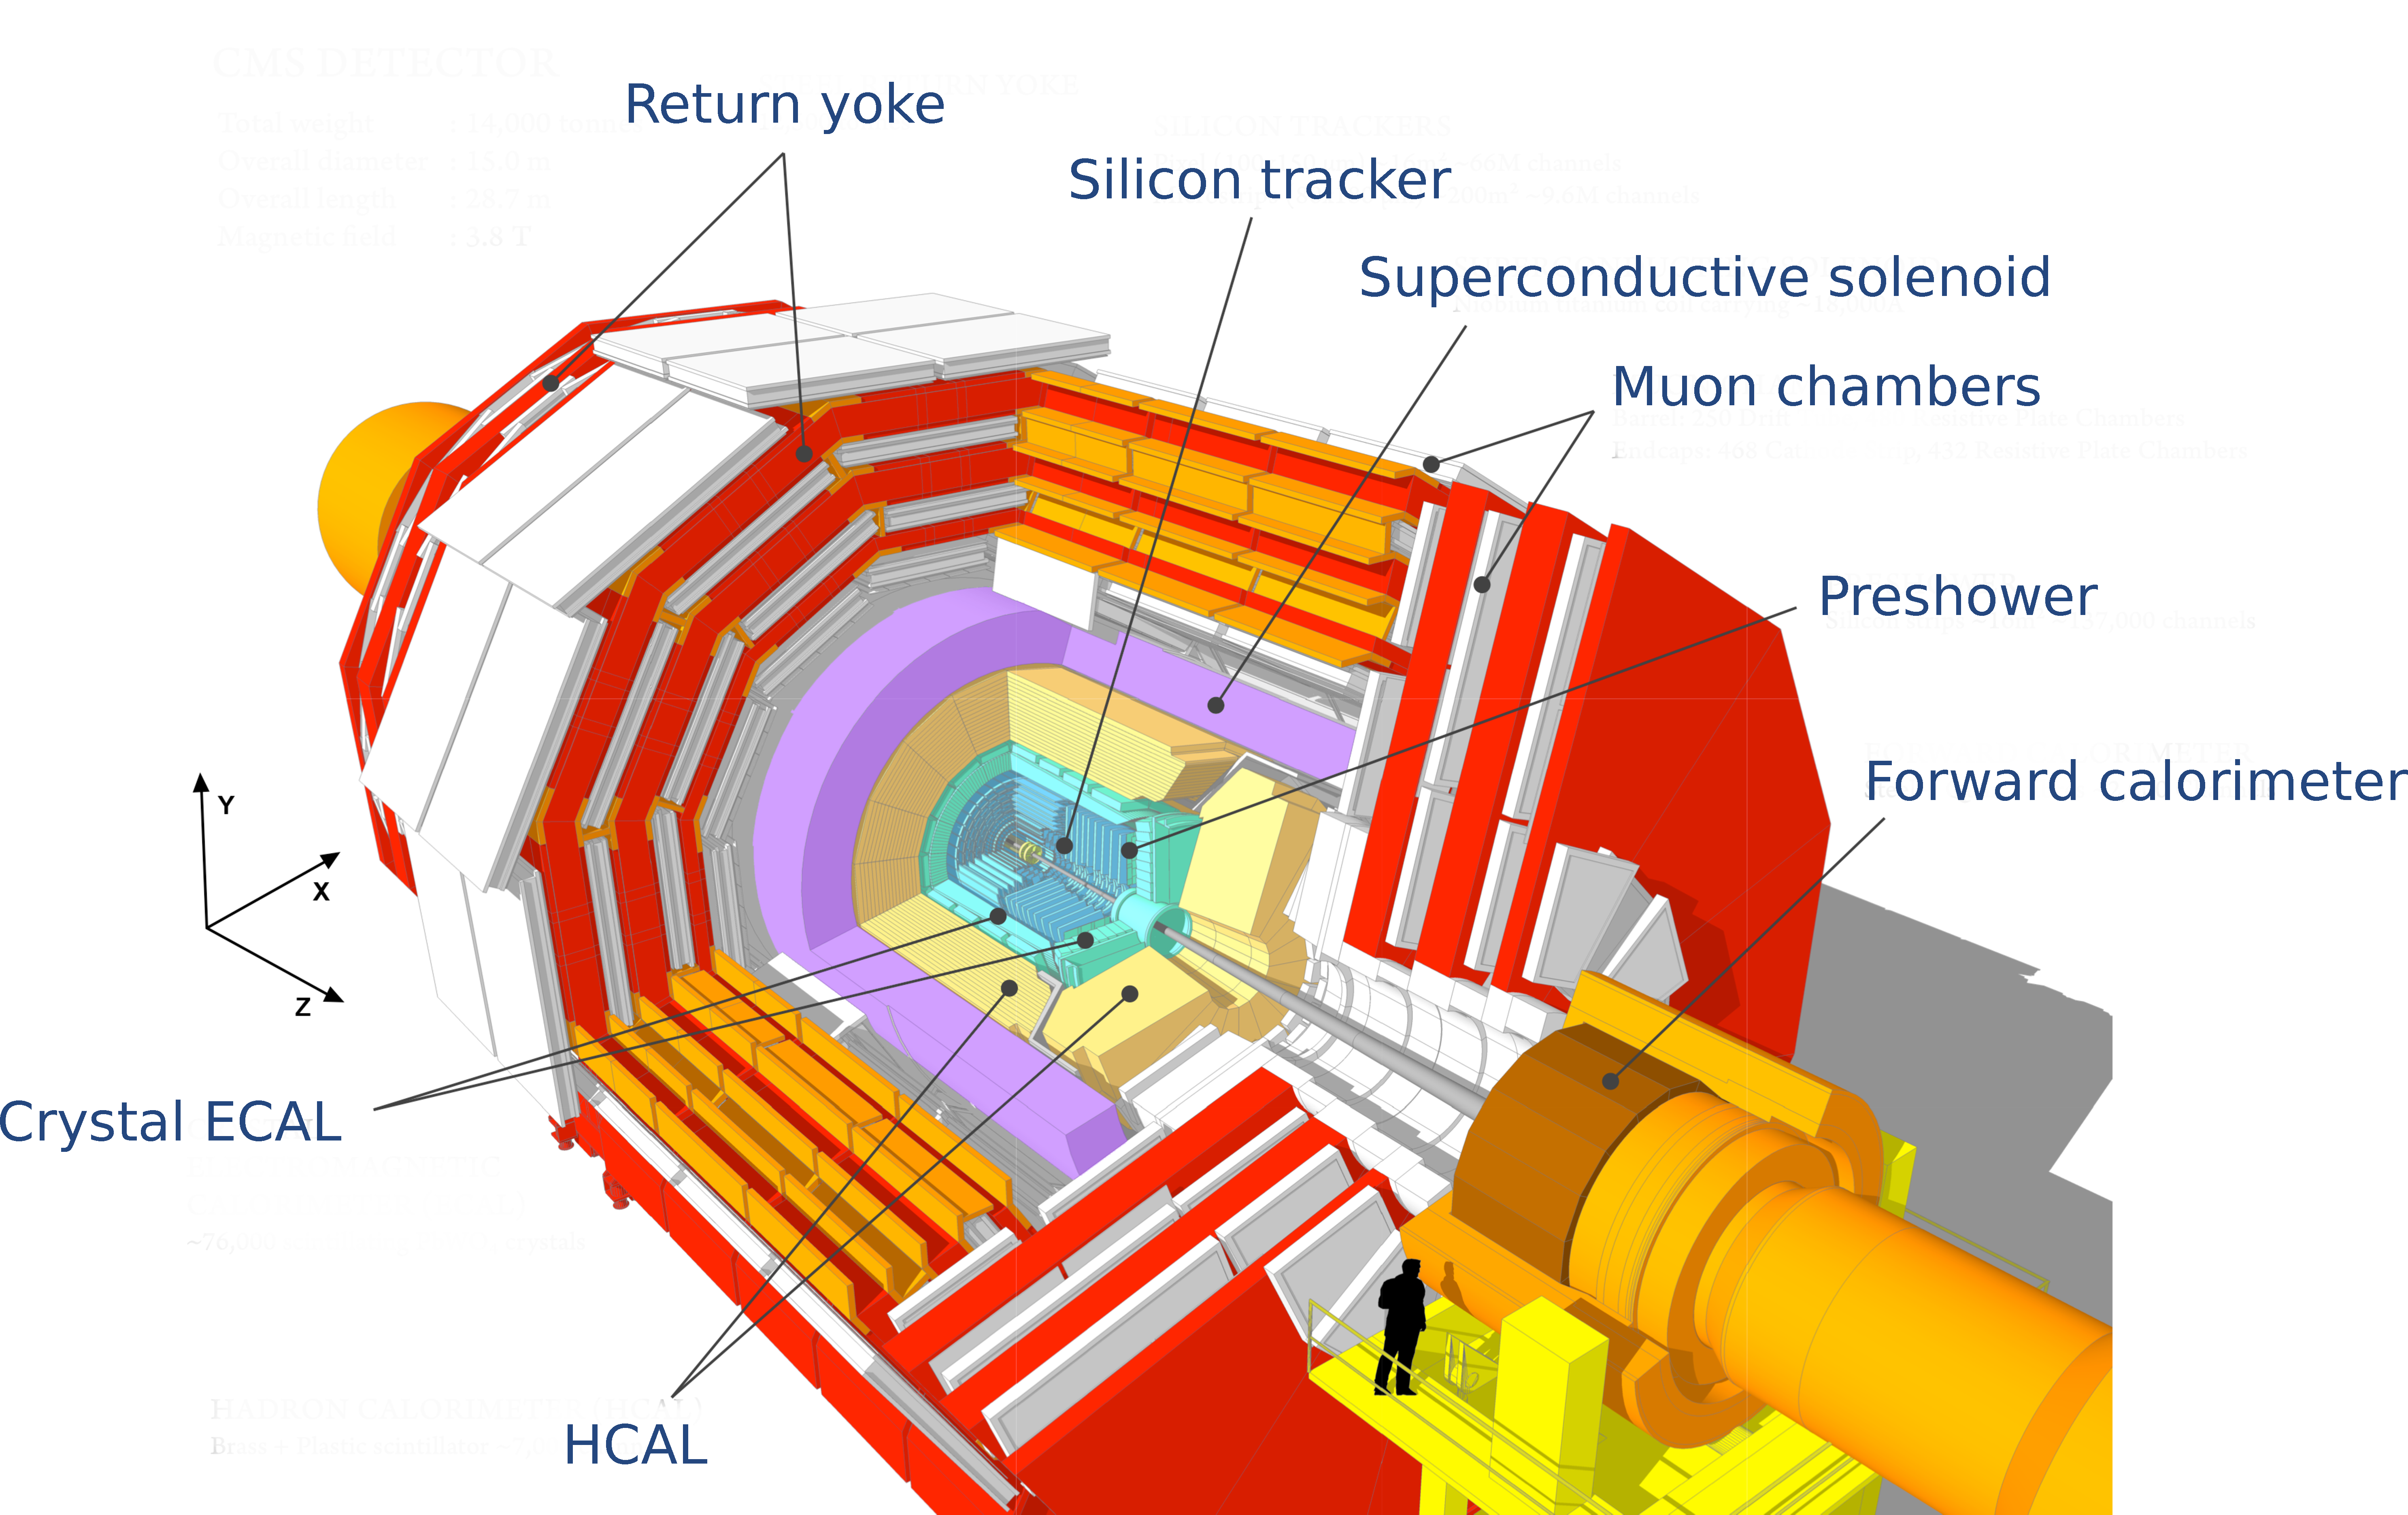
\includegraphics[width=0.75\linewidth]{fig/chapt2/CMS_detail.pdf}
		\caption{\label{fig:CMS-detail} View of the CMS apparatus and of its different components.}
	\end{figure}
	
	\begin{figure}[H]
		\centering
		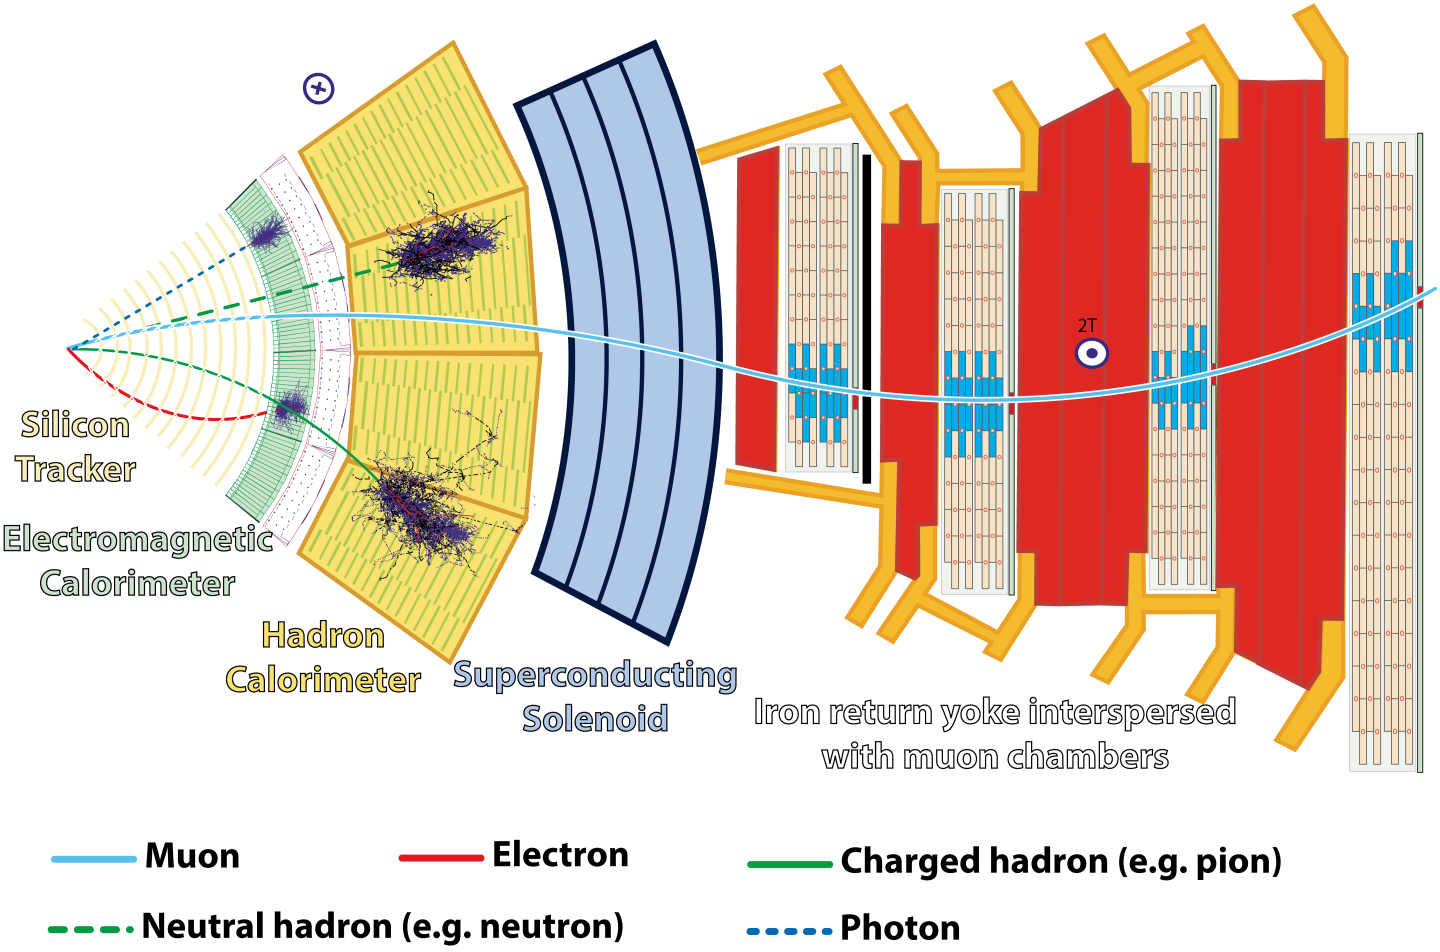
\includegraphics[width=0.8\linewidth]{fig/chapt2/CMS_slice.png}
		\caption{\label{fig:CMS-slice} Slice showing CMS sub-detectors and how particles interact with them.}
	\end{figure}
	
		\subsubsection{The silicon tracker}
		\label{chapt2:sssec:tracker}
	
\begingroup\setlength{\intextsep}{5pt}\setlength{\columnsep}{15pt}
	
	\begin{wrapfigure}{r}{.65\linewidth}
		\centering
		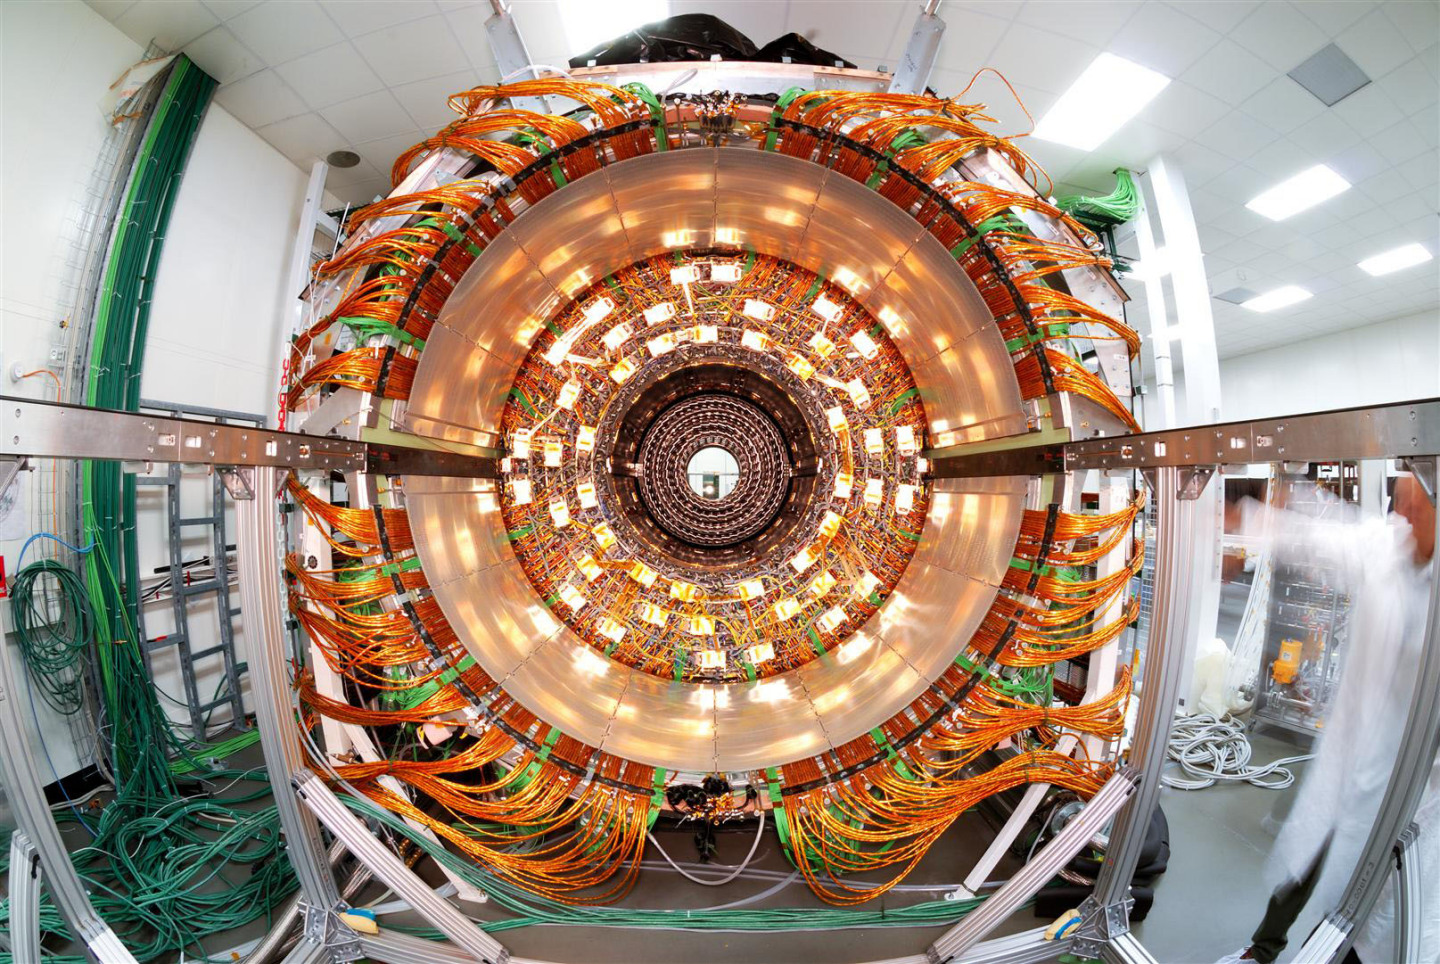
\includegraphics[width = \linewidth]{fig/chapt2/Tracker.jpg}
		\caption{\label{fig:tracker} The CMS tracker.}
	\end{wrapfigure}
	
	The silicon tracker visible in Figure~\ref{fig:tracker} is divided into two different sub-systems: the \textit{pixel detector} at the very core and the \textit{microstrip detector} around it. This system is composed of 75 million individual readout channels with up to 6000 channels per squared centimeter for the pixels making it the world's biggest silicon detector. This density allows for measurements of the particle tracks with a precision of the order of \SI{10}{\mu m}. This is necessary to reconstruct all the different interaction vertices with precision and have a precise measure of the curvature of the charged particles traveling through the magnetic field to estimate their charge and momentum.
	
\endgroup
	
		\subsubsection{The calorimeters}
		\label{chapt2:sssec:calo}
	
	The ECAL directly surrounding the tracker is composed of crystals of lead tungstate, $PbWO_4$, a very dense but optically transparent material used to stop high-energy electrons and photons. These crystal blocks basically are extremely dense scintillators which scintillate in fast, short light bursts proportionally to the energy deposition. The light is contained at 80\% in the corresponding \SI{25}{ns} lasting bunch crossing. Each crystal is isolated from the other by the carbon fiber matrix they are embedded in.
	
	\begin{figure}[H]
		\begin{subfigure}{.5\linewidth}
			\centering
			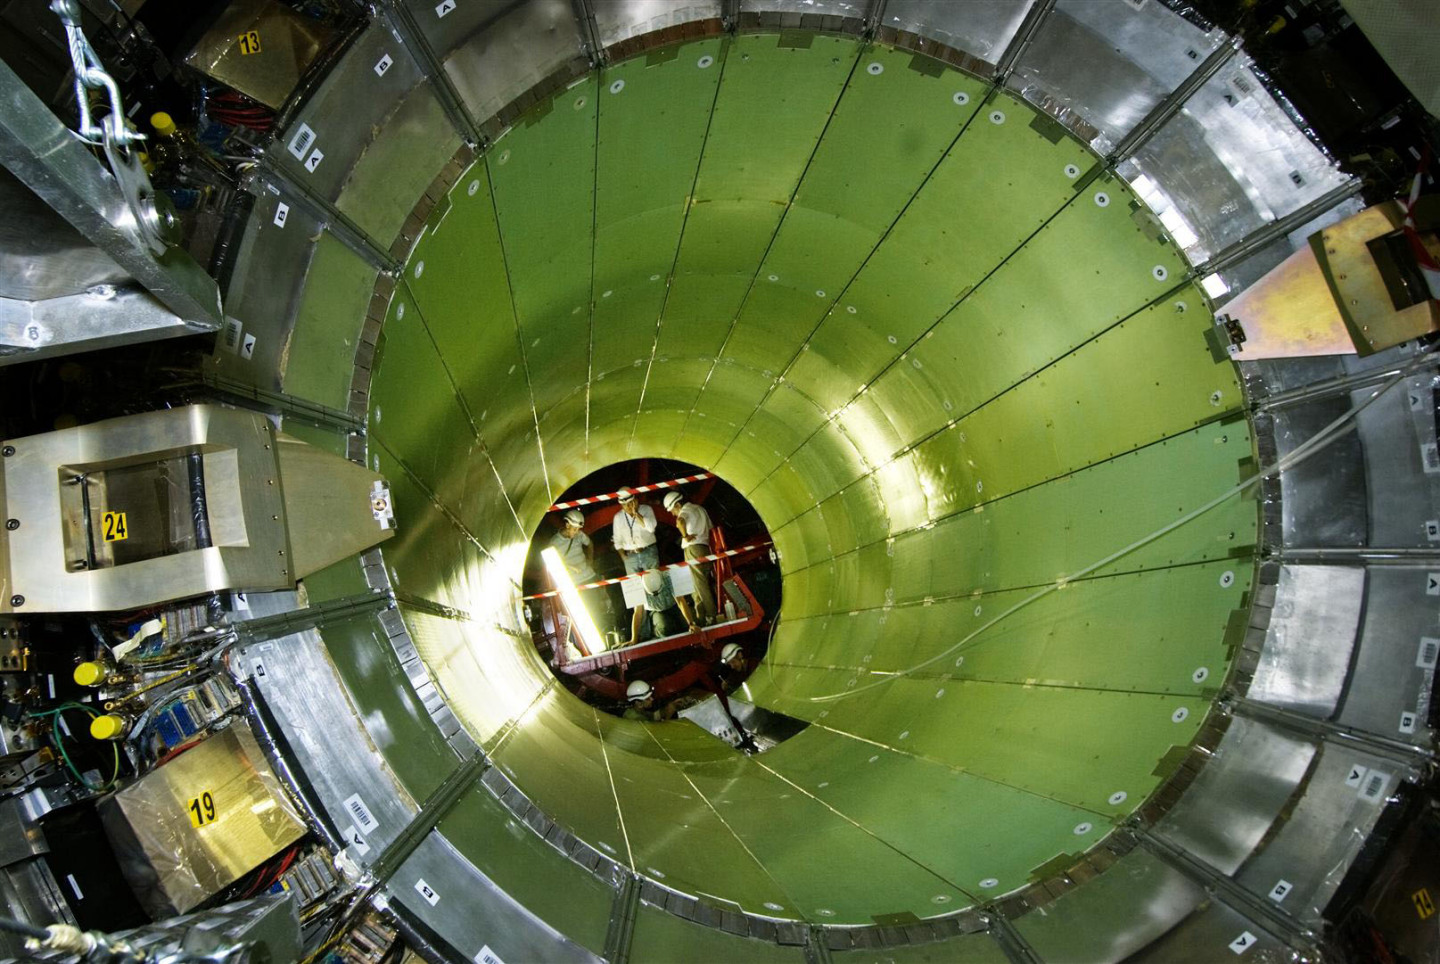
\includegraphics[height = 4.5cm]{fig/chapt2/ECAL_barrel.jpg}
			\subcaption{\label{fig:ECAL:A}}
		\end{subfigure}
		\begin{subfigure}{.5\linewidth}
			\centering
			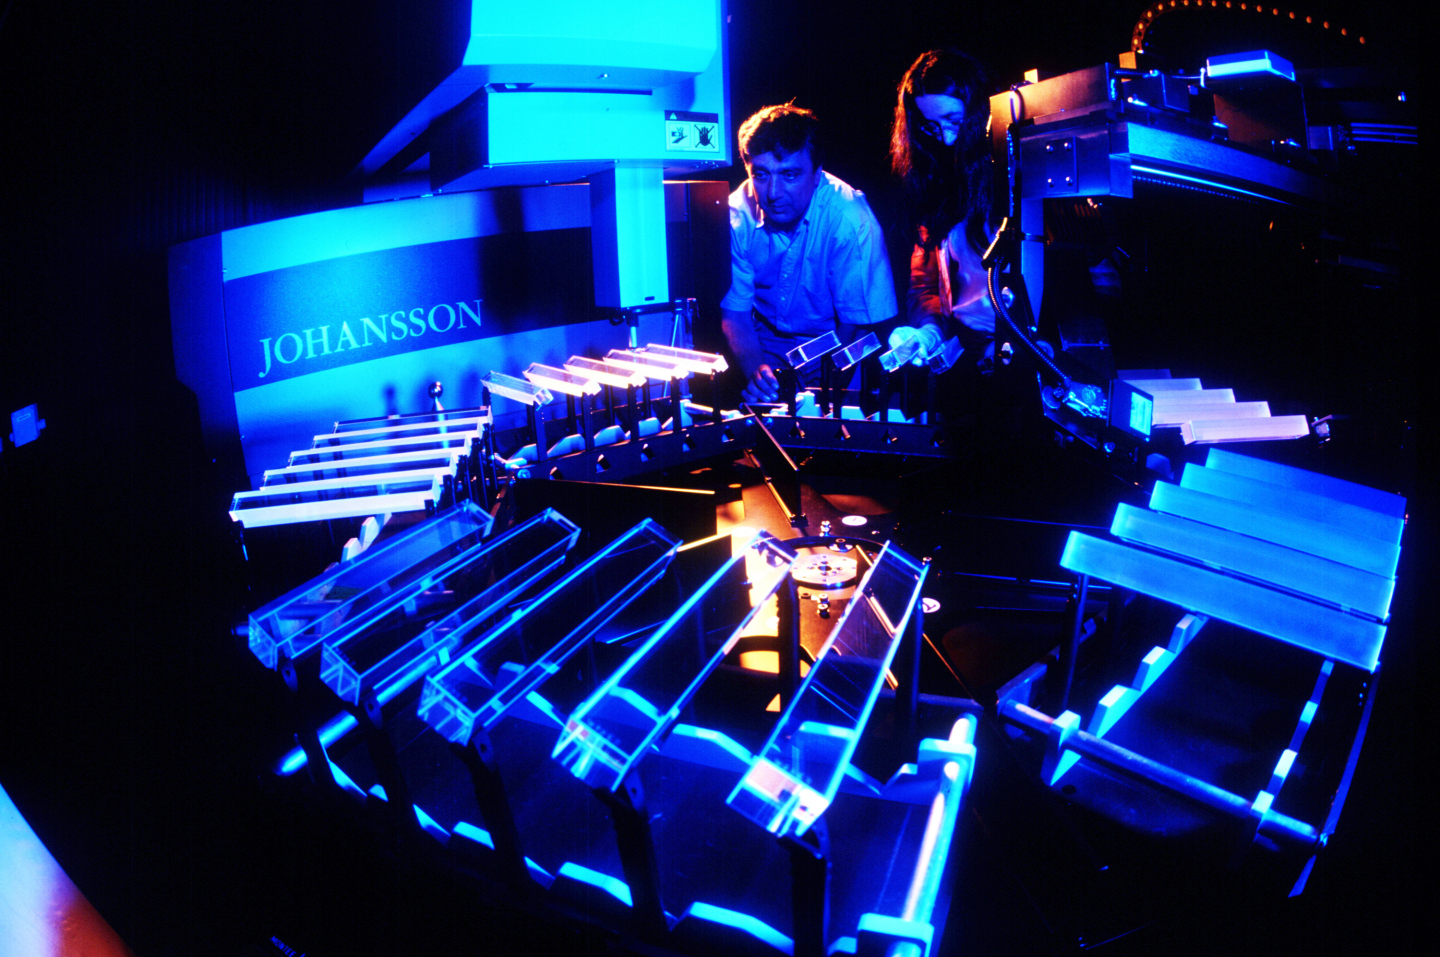
\includegraphics[height = 4.5cm]{fig/chapt2/ECAL_crystals.jpg}
			\subcaption{\label{fig:ECAL:B}}
		\end{subfigure}
		\caption{\label{fig:ECAL} Figure~\ref{fig:ECAL:A}: The \acl{ECAL}. Figure~\ref{fig:ECAL:B}: The lead tungstate crystals composing the ECAL.}
	\end{figure}
	
\begingroup\setlength{\intextsep}{5pt}\setlength{\columnsep}{15pt}
	
	\begin{wrapfigure}{r}{.5\linewidth}
		\centering
		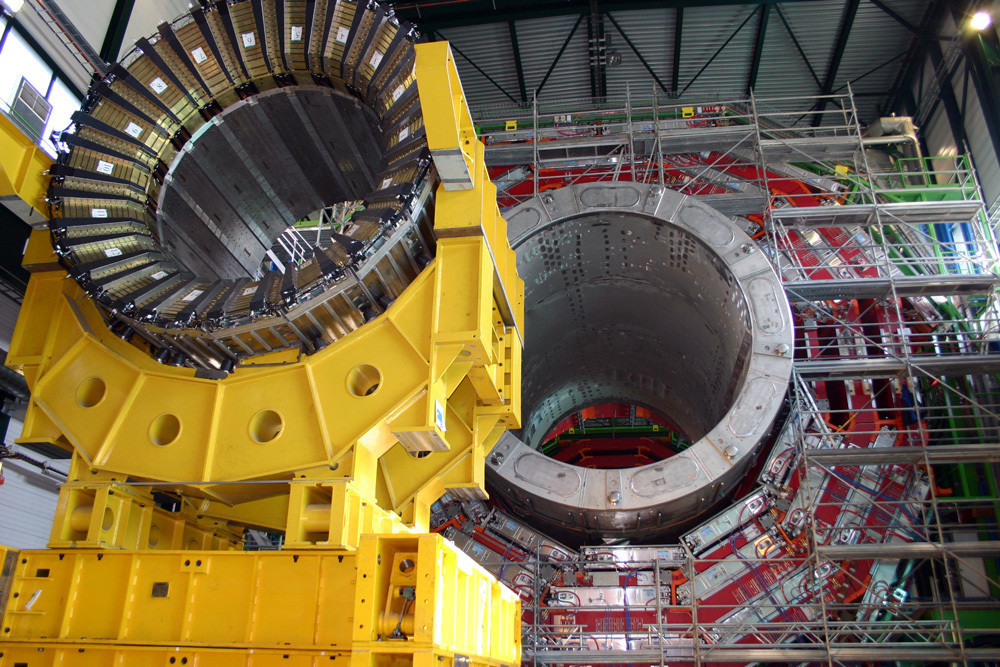
\includegraphics[width = \linewidth]{fig/chapt2/HCAL.jpg}
		\caption{\label{fig:HCAL} The CMS hadron calorimeter barrel.}
	\end{wrapfigure}
	
	The ECAL is composed of a barrel containing more than 60,000 crystals and of closing endcaps containing another 15,000 crystals. In front of the ECAL endcap is installed a preshower detector made out of two layers of lead and silicon strip detectors to increase the spatial resolution close to the beam line for pion-photon and single-double photon discrimination purposes. Figure~\ref{fig:ECAL} shows the calorimeter inside of the magnet and the crystals.
	
	The next layer is the HCAL. The role of these forward calorimeters, made using steel and quartz fibers, is to precisely measure the momentum very energetic hadrons. Several layers of brass or steel are interleaved with plastic scintillators readout by photodiodes using wavelength-shifting fibers. The HCAL is also composed of a barrel, shown in Figure~\ref{fig:HCAL} and of endcaps. It also features forward calorimeters on both sides of CMS in the region very close to the beam line at high pseudorapidity (\psrapr{3.0}{5.0}).
	
\endgroup
	
		\subsubsection{The muon system}
		\label{chapt2:sssec:muon}
	
	Finally, in the outer region of the apparatus, a muon system is used to trigger on potentially interesting event by identifying muons. Three different subsystems compose the muon system as shown in Figure~\ref{fig:Quadrant} in which a quadrant of the CMS detector focuses on muon system. \acl{DT}s (DTs) are found in the barrel region covering the low pseudorapidity region where particles transverse momentum is lower and \acl{CSC}s (CSCs) are found in the endcap region covering higher pseudorapidity region closer to beam line where particles have a stronger momentum. The redundancy of the system is insured by \acl{RPC}s (RPCs) in both the barrel and endcap. Nevertheless, the region closest to the beam line (\psrapg{1.8}) was not equipped with RPCs. This lack of redundancy in the high pseudo rapidity region will be solved during LS2, the following \acf{YETS} in 2021 and 2022, and LS3 where the necessary services, detectors and Link System, that collects the data and synchronizes them, will be installed.

	\begin{figure}[H]
		\centering
		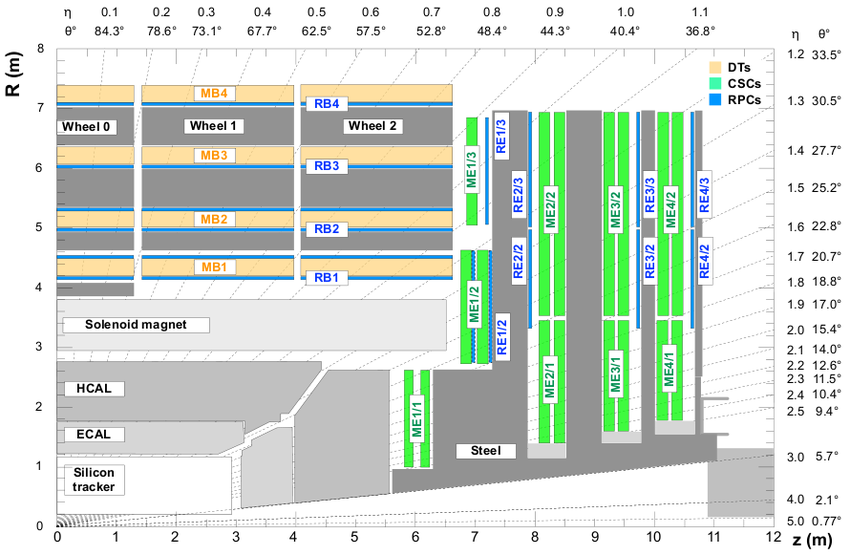
\includegraphics[width=0.9\linewidth]{fig/chapt2/Muon_quadrant.png}
		\caption{\label{fig:Quadrant} A quadrant of the muon system, showing DTs (yellow), RPCs (blue), and CSCs (green).}
	\end{figure}

\clearpage{\pagestyle{empty}\cleardoublepage}